\documentclass{report}
\usepackage[utf8]{inputenc}
\usepackage{mathrsfs}
\usepackage{caption}

\usepackage{graphicx} % Required for inserting images
\graphicspath{{img/}}
\usepackage[a4paper,top=2cm,bottom=2.5cm,left=2.5cm,right=2.5cm,marginparwidth=0cm]{geometry}

%link in latex
\usepackage[hidelinks]{hyperref}
\hypersetup{
    colorlinks=false,
    linkcolor=blue,
    filecolor=magenta,      
    urlcolor=cyan,
    pdftitle={Operating_System_Appunti_Berardo_Cristiano},
    pdfpagemode=FullScreen,
    }
\urlstyle{same}
\usepackage{afterpage}
\usepackage[T1]{fontenc} % codifica dei font
\usepackage[utf8]{inputenc} % lettere accentate da tastiera
\usepackage[english]{babel} % lingua del documento
\usepackage{url} 
\usepackage{quoting}
\usepackage{xspace}% per lo spazio intelligente
\usepackage{titlesec} % per formato custom dei titoli dei capitoli
\usepackage{tcolorbox}%per i box

\usepackage{float}
\usepackage{sidecap}
\usepackage{amsmath}
\usepackage{pgfplots}   % per i grafici
\pgfplotsset{width=7cm,compat=1.9}
\usepackage{booktabs}
\usepackage{amssymb}

\usepackage{circuitikz}


\usepackage[T1]{fontenc}





\usepackage{listings}
\usepackage{textcomp}
\usepackage{xcolor}

\definecolor{codegreen}{rgb}{0,0.6,0}
\definecolor{codegray}{rgb}{0.5,0.5,0.5}
\definecolor{codepurple}{rgb}{0.58,0,0.82}
\definecolor{backcolour}{RGB}{247, 246, 243}
\definecolor{my_yellow}{RGB}{178, 173, 85}


% \lstdefinestyle{mystyle}{
%     backgroundcolor=\color{backcolour},   
%     commentstyle=\color{codegreen},
%     keywordstyle=\color{magenta},
%     numberstyle=\tiny\color{codegray},
%     stringstyle=\color{codepurple},
%     basicstyle=\ttfamily\footnotesize,
%     breakatwhitespace=false,         
%     breaklines=true,                 
%     captionpos=b,                    
%     keepspaces=true,                 
%     numbers=left,                    
%     numbersep=5pt,                  
%     showspaces=false,                
%     showstringspaces=false,
%     showtabs=false,                  
%     tabsize=2
% }

\usepackage{color}
\definecolor{pblue}{rgb}{0.13,0.13,1}
\definecolor{pgreen}{rgb}{0,0.5,0}
\definecolor{pred}{rgb}{0.9,0,0}
\definecolor{pgrey}{rgb}{0.46,0.45,0.48}



% ------------- CODE IN JAVA ---------------------
\lstdefinestyle{style1}{
    language=Java,
    numberstyle=\tiny\color{codegray},
    numbers=left,
    backgroundcolor=\color{backcolour},   
    showspaces=false,
    showtabs=false,
    breaklines=true,
    showstringspaces=false,
    breakatwhitespace=true,
    commentstyle=\color{pgreen},
    keywordstyle=\color{pblue},
    stringstyle=\color{pred},
    basicstyle=\ttfamily,
    moredelim=[is][\textcolor{pgrey}]{\%\%}{\%\%}
}
\lstdefinestyle{codeinjava}{
    style=style1,
}
\lstnewenvironment{codeInJava}{
    \lstset{
        style=codeinjava,
    }
}{}

% ------------- END CODE IN JAVA ---------------------

% ------------- START CODE IN C/C++ ---------------------

\lstdefinestyle{style2}{
    numbers=left,
    belowcaptionskip=1\baselineskip,
    breaklines=true,
    xleftmargin=\parindent,
    language=C,
    % identifierstyle=\color{blue},
    stringstyle=\color{orange},
    backgroundcolor=\color{backcolour},   
    commentstyle=\color{codegreen},
    keywordstyle=\color{pblue},
    numberstyle=\tiny\color{codegray},
    stringstyle=\color{codepurple},
    basicstyle=\ttfamily,
    breakatwhitespace=false,         
    breaklines=true,                 
    captionpos=b,                    
    keepspaces=true,                 
    numbers=left,                    
    numbersep=5pt,                  
    showspaces=false,                
    showstringspaces=false,
    showtabs=false,                  
    tabsize=2
}

\lstdefinestyle{codeinc}{
    style=style2,
}

\lstnewenvironment{codeInC}{
    \lstset{
        style=codeinc,        
    }
}{}

\lstdefinestyle{style3}{
  belowcaptionskip=1\baselineskip,
  frame=L,
  xleftmargin=\parindent,
  language=[x86masm]Assembler,
  basicstyle=\footnotesize\ttfamily,
  commentstyle=\itshape\color{purple!40!black},
}

% ------------- END CODE IN C/C++ ---------------------


%\lstset{style=mystyle}







\newcommand\blankpage{%
    \null
    \thispagestyle{empty}%
    \addtocounter{page}{-1}%
    \newpage}

\begin{document}

\pagestyle{plain}

\thispagestyle{empty}

\begin{center}
  \begin{figure}[h!]
  \centering
    
\includegraphics[trim= 1cm 3.5cm 8.1cm 24.2cm, clip]{img/unitnlogo.pdf}
  \end{figure}

  \vspace{2 cm} 

  \LARGE{Dipartimento di Ingegneria e Scienza dell’Informazione\\}

  \vspace{1 cm} 
  \Large{Corso di Laurea in\\
    %Informatica
    Ingegneria Informatica, delle Comunicazioni ed Elettronica
    %Ingegneria dell'Informazione e Organizzazione d'Impresa
    %Ingegneria Elettronica e delle Telecomunicazioni
  }

  \vspace{2 cm} 
  %\Large\textsc{Manuale di Fisica I\\} 
  %\vspace{1 cm} 
  \Huge\textsc{Operating System\\}
  %\Large{\it{Con un approccio da studente a studente}}


  \vspace{2 cm} 
  \begin{tabular*}{\textwidth}{ c @{\extracolsep{\fill}} c }
  \Large{Docente} & \Large{Studente}\\
  \Large{Tommaso Zoppi}& \Large{Cristiano Berardo 234428}\\
  \end{tabular*}

  \vspace{2 cm} 

  \Large{Anno accademico 2023/2024}
  
\end{center}
\afterpage{\blankpage}


\tableofcontents

\clearpage


% /*\part{Introduction to Operating System}
% \newpage*/
\chapter{What is Operating System?}

Operating System is a combination of two parts:

\begin{itemize}
    \item Hardware;
    \item Software;
\end{itemize}

Operating System is a program that acts as intermediary between a user of a computer and the computer hardware.

The main goal of OS are:

\begin{itemize}
    \item Execute user program and make solving user problems easier;
    \item Use the computer hardware in an efficient manner;
    \item Make the computer system easier to use;
\end{itemize}

To sum up, an OS provides an environment in which other software can do
useful work.
A computer System consists on 4 components: HW, SO, Applications and
Users.
The Operating System coordinates Hardware and Applications.
An OS is also a resource allocator (it manages all resources), and a control program (it controls
the execution of programs to prevent errors and improper use of the computer).

\begin{figure}[htbp]
    \centering
    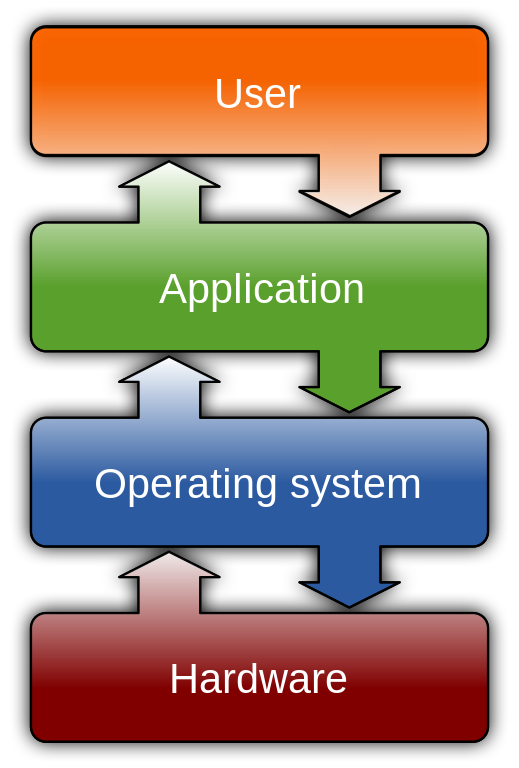
\includegraphics[scale=0.2]{img/Operating_system.png}
    % \caption{Propagazione onde elettromagnetiche}
    % \label{OndeElettromagentiche}
\end{figure}

\newpage
\section{Computer System}
A Computer system when booted up launches a procedure called bootstrap which launches the
OS kernel and starts execution.

\begin{figure}[htbp]
    \centering
    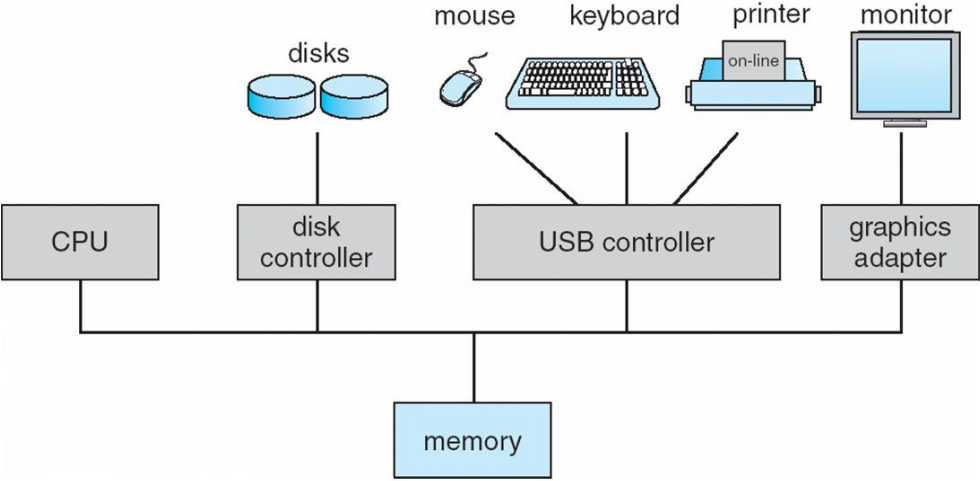
\includegraphics[scale=0.30]{img/cs.png}
\end{figure}

\subsection{How do all these things work together?}
Device controller informs the
CPU that it has finished its
operation by causing an
interrupt, an event in the OS.

\begin{figure}[htbp]
    \centering
    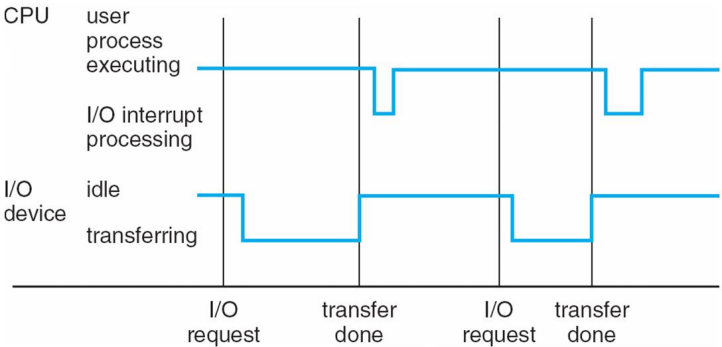
\includegraphics[scale=0.45]{img/inter.png}
\end{figure}

Example: when you try to
transfer data, the CPU is
notified when the device (may
be a pen drive) has finished to
transfer all the data through a
message of interrupt.

Every interrupt message has a memory address associated. The table that determines all of these
addresses is generated at startup.
When an interrupt occurs, the CPU saves the current Program Counter (PC) value and jumps to
the first instruction of the routine to handle the interrupt, executes the routine and then jumps
back to where the PC was. We can say that an OS is interrupt driven.

What if the CPU is doing something very important when an interrupt message arrives?
There are two types of interrupt:

\begin{itemize}
    \item Maskable interrupts: can be handled whenever critical instructions are being executed;
    \item Non-maskable interrupts: have high priority and have to be handled right as they arrive;
\end{itemize}

The structure of interrupt implies that CPU has to manage I/O processes after the transfer of each
portion of data has been executed, we don’t want that.
The DMA (Direct Memory Access) manages the data transfer and notifies the CPU only after
everything is finished

\newpage
\section{Memory}

\begin{itemize}
    \item \textbf{Cache - SRAM}: it is really fast but expensive (1 ns latency). It’s the first memory che CPU checks when
searching for a piece of information. It is \textit{volatile};
    \item \textbf{Main memory - DRAM}: large storage media that the CPU can access directly (DRAM), typically volatile
(20 ns latency). It is \textit{volatile};
    \item \textbf{Secondary storage - HDD/Flash NAND}: extensions of the main memory (non volatile) such as HDD and SSD
($250\,000$ ns latency). It is  \textit{not volatile};
\end{itemize}

\textbf{Caching}: copying information into faster storage system. Main memory can be viewed as a cache
for secondary storage.
For example, if the CPU finds the information in the main memory, it copies that information into
the cache so it can be accessed faster.

\begin{figure}[htbp]
    \centering
    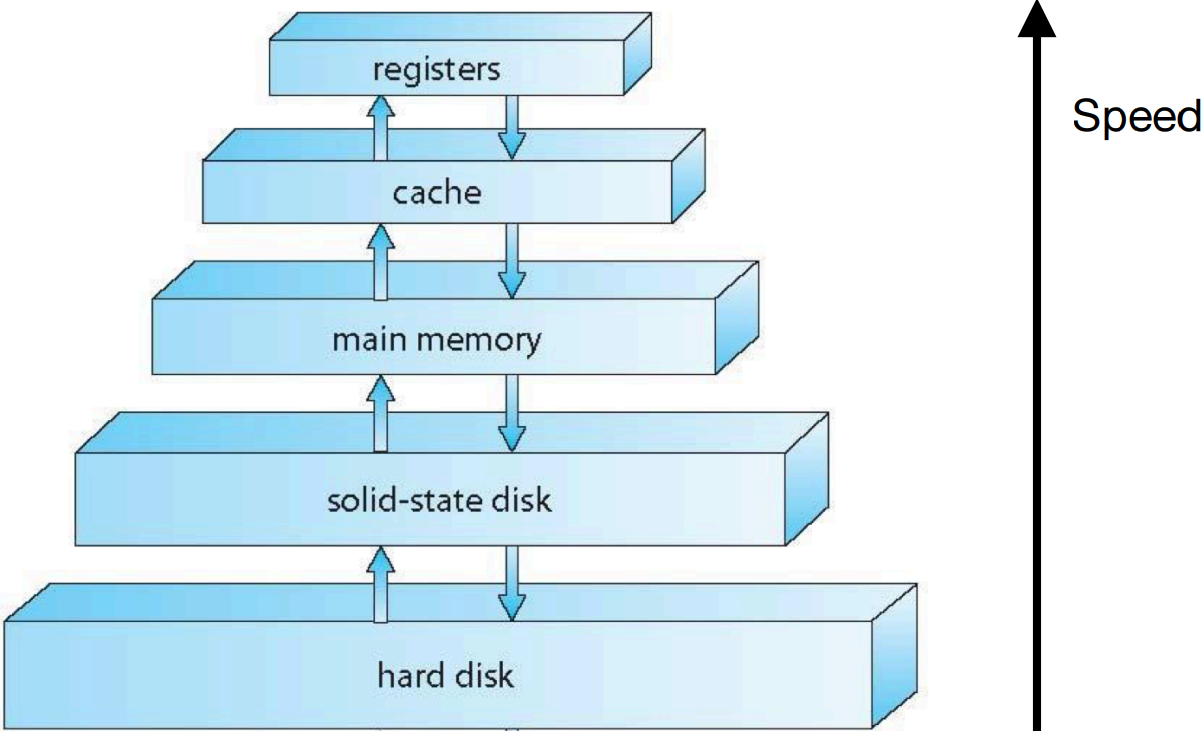
\includegraphics[scale=0.25]{img/mem.png}
\end{figure}

Without main memory and cache every time we have to access data we have to search it into
secondary memory, which is much slower.

\subsection{Performance of various levels of storage}


\begin{figure}[htbp]
    \centering
    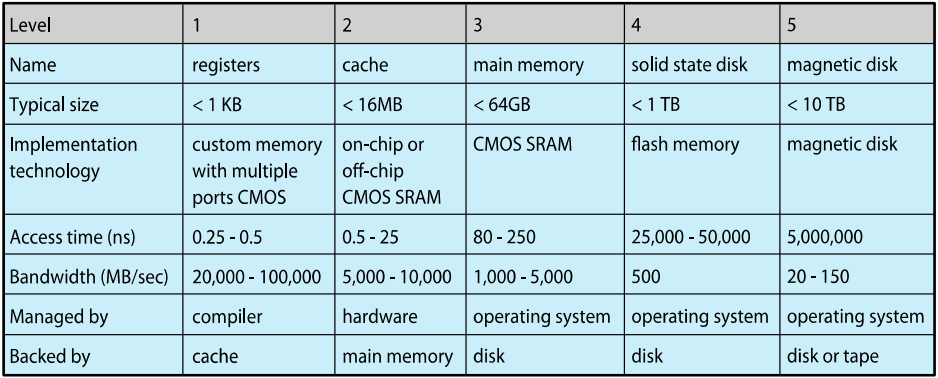
\includegraphics[scale=0.55]{img/stor.png}
\end{figure}

\newpage
\section{Modern system architectures: how a computer works}

First idea of a computer by Von Neumann is: Device comunicate with CPU and CPU comunicate with memory. This first idea is un-efficient because every input bother the CPU, so now device use the DMA (Direct Memory Access) to bypass CPU to send or to receve data directly to or from the main memory.

\begin{figure}[htbp]
    \centering
    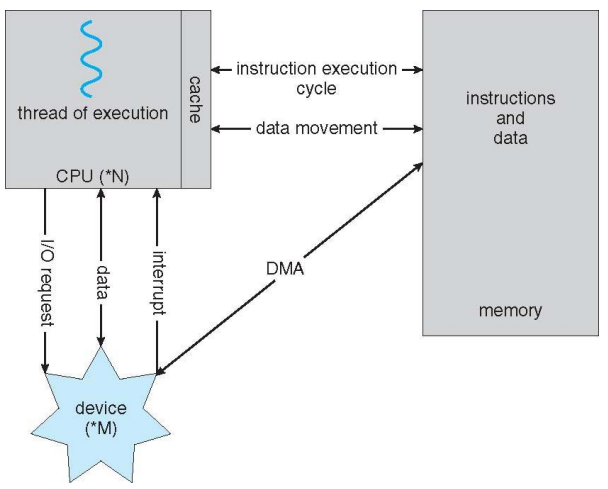
\includegraphics[width=0.65\linewidth]{img/cpu.png}    
\end{figure}


\subsection{Processor}

Lot of system use a single general-purpose processor. 
There are two different type of processors:

\begin{itemize}
    \item Multi-processor, each processor, with one core, has its own cache and register
    \item Multi-core, each core in the chip share cache and register with other core
\end{itemize}

\paragraph{}
Also there are two different way to work for multiple tasks:

\begin{itemize}
    \item Asymmetric processing (specific task)
    \item Symmetric processing (random tasks)
\end{itemize}


\subsubsection{Asymmetric Multi-processor}
Each processor, with one core each, is assigned a specific task. After performing the task, the processor waits another specific task and does not help other processors.

\subsubsection{Symmetric Multi-processor}
Each processor, with one core each, is assigned a random task. After performing the task, the processor helps the other processors and improves the overall performance.

\subsubsection{Asymmetric Multi-Core}
It is single chip, with several core inside. Each core works on a specific task and after performing the assigned specific tasks waits, without helping the other cores, for other specific tasks. 

\subsubsection{Symmetric Multi-Core}
It is single chip, with several core inside. Each core works on a random tasks and if one or more cores perform the task, the core helps the others, thus improving the overall performance.


\begin{figure}[htbp]
    \centering
    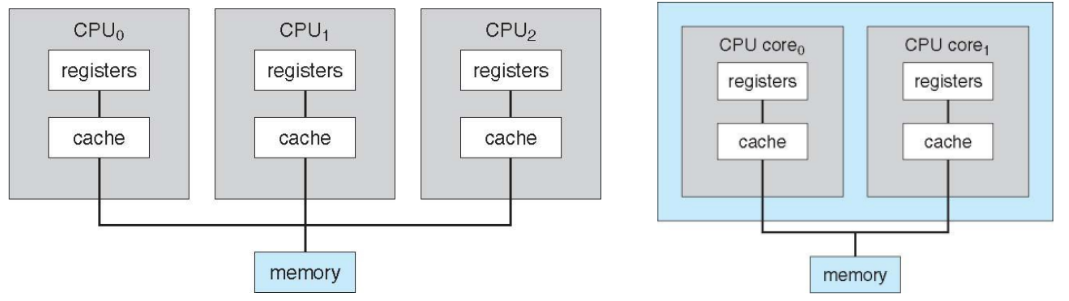
\includegraphics[width=1\linewidth]{img/multiP.png}
    \caption{Multi-processor on the left; Multi-Core on the right}
\end{figure}

\subsubsection{Is not it the same, why modern system are multi-core?}

\begin{itemize}
    \item On-Chip buses are faster;
    \item Single chip required less power;
    \item If one core die you throw the CPU in the bin
\end{itemize}

\subsection{High performance computer \textbf{HCP}}
If you do not care about power consumption and want a powerful machine because you are Google, Amazon etc., you should consider to build a Cluster.
A cluster is group of many computers, even with different OS, working together to complete tasks, such as cloud computing.
The application must be written to use parallelization.
\begin{figure}[htbp]
    \centering
    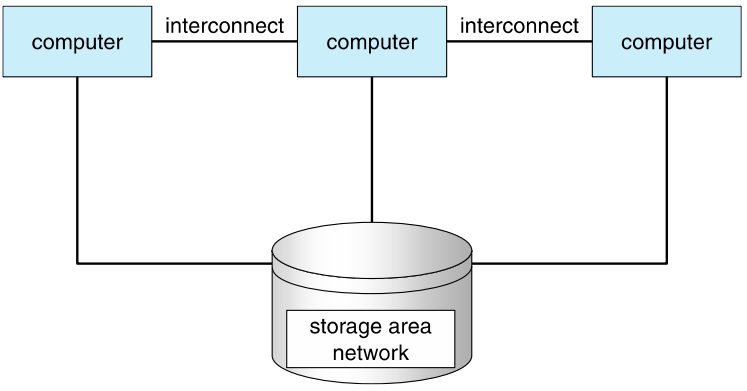
\includegraphics[width=0.6\linewidth]{img/SAN.png}
    \caption{SAN}
\end{figure}

Also Cluster server can chose with type of implementation to use:

\begin{itemize}
    \item Asymmetric: each machine has a hardware copy of the first machine, and if the first computer brakes the other machine, in hot-standby, starts working.
    \item Symmetric: has multiple nodes running applications, monitoring each other, if one brakes another machine takes its place.
\end{itemize}

\newpage

\section{Startup}
When you turn on the PC lots of things happen:

\begin{itemize}
    \item The bootstrap routine is invoked
    \item It stays in a pre-defined portion of the memory (firmware)
    \item The bootstrap routine initializes registers, memory and device controllers
    \item Calls the kernel and puts it in the main memory
    \item Starts daemons i.e., programs not in the kernel but that have to be run at startup like start and initialize driver for the monitor
    \item Once everything is ready, the OS is ready to provide an environment in which processes can be run
    \item A process is a program in execution
\end{itemize}

\subsection{Improve performance}


Executes multiple programs concurrently on a single CPU with one core need to improve efficiency.
There are two methods to improve performance: \textbf{Multiprogramming} and \textbf{Timesharing}


\subsubsection{Multiprogramming (Batch system)}

Think to have one processor with one core, system can not waste time, like wait for I/O. Multiprogramming organise tasks to do (code and data) so always CPU has something to do.
A subset of total jobs in system is kept in memory and when CPU has to wait (I/O), OS switches to another job.

Doesn't actually create the illusion of simultaneous execution for users.

\subsubsection{Timesharing (multitasking)}

Is logical extension in which CPU switches jobs so frequently that users can interact with each job while it is running, creating
interactive computing.
Users feel like they are interacting with their programs simultaneously, even though the CPU is only working on one program at a time.

We can also decide how to execute programs: by always finishing executing program-N or by starting to work first with the program that requires  the shortest execution time, or, like in the previous paragraph, by switching between different tasks.

\subsection{Switching Mechanism}

\subsubsection{Multiprogramming (Batch system)}

\begin{itemize}
    \item Relies on I/O events (like waiting for data from disk) to switch between processes.
    \item When the currently running program needs to wait for I/O, the CPU switches to another program that's ready to run.
\end{itemize}

\subsubsection{Timesharing (multitasking)}

\begin{itemize}
    \item Uses a time-slicing mechanism to switch between processes.
    \item The operating system allocates a short time slice (quantum) to each process, and after the quantum expires, it switches to the next ready process, regardless of its need for I/O.
\end{itemize}

In summary, while both multiprogramming and timesharing improve resource utilization, timesharing adds the concept of time slicing to create the illusion of simultaneous execution for multiple users, making it more user-friendly and interactive.


\newpage
\subsection{Security and OS protection}
Two different levels to interact with system function:

\begin{itemize}
    \item User mode (only some privileges decided by company or others admins)
    \item kernel mode (all privileges)
\end{itemize}

\begin{figure}[htbp]
    \centering
    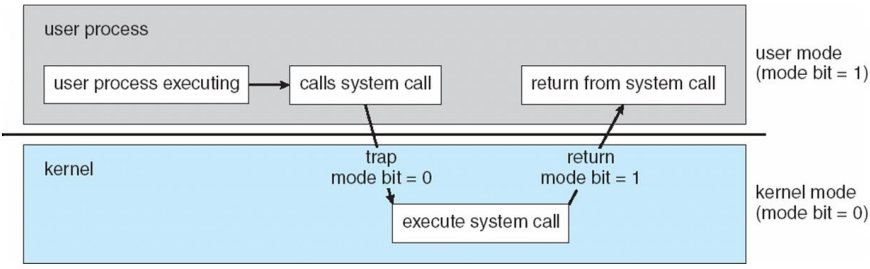
\includegraphics[width=0.8\linewidth]{img/secur.png}
\end{figure}

\paragraph{}
\begin{itemize}
    \item \textbf{Protection} – any mechanism for controlling access of processes or users to resources defined by the OS
    \item \textbf{Security} – defense of the system against internal and external attacks
\end{itemize}

System first distinguish users to determinate who can do what using: user IDs and group ID


An attach can threat to:
\begin{itemize}
    \item Confidentiality: absence of unauthorized disclosure of information
    \item Availability: service availability (CPU detect and stop malicious process)
    \item Integrity: absence of improper system alterations
\end{itemize}




\subsection{Program counter}
\begin{itemize}
    \item Single-threaded process has one program counter specifying location of next instruction to execute
    \item Multi-threaded process has one program counter per thread
\end{itemize}

\subsection{Storage Management}

OS provide to manage traffic data from RAM to SSD and vice versa, also OS give the impression that it is organise in directory.

\begin{itemize}
    \item \textbf{Multitasking} environments must be careful to use most recent
value, no matter where it is stored in the storage hierarchy
    \item \textbf{Multiprocessor} environment must provide cache coherency in
hardware such that all CPUs have the most recent value in their
cache
\end{itemize}



\chapter{Operating-System Structures}

OS has the task of interconnecting HW and SW. It provides function that are helpful to the user: system call, services, user interface, I/O, file system, network interface, error detection, resource allocation, security and so on.

\begin{figure}[htbp]
    \centering
    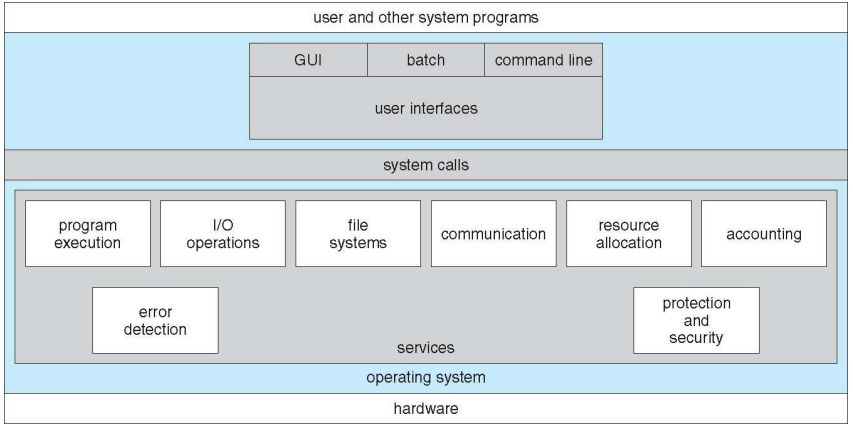
\includegraphics[width=0.7\linewidth]{img/SO.png}
\end{figure}

\section{Operating System Services }

\subsection{(G)UI}

CLI or command line interface allows detect command entry. The basic CLI in windows is Command Prompt, also known as cmd.exe or cmd. CLI existing in each OS (Windows, Max, Linux and Solaris etc.).

Nowadays the UI is more user-friendly tanks the graphics, programme icons, button, directory, files etc. Even if  OS now include GUI, they also have the old CLI.


\newpage
\section{System Calls}
System Calls are typically written in high-level language (C, C++). Most libraries include specific functions that allows programmers to call the operating system call. 

Most common API are:
\begin{itemize}
    \item Win32 API for Windows
    \item POSIX API for POSIX-based systems (UNIX, Linux and Max OS X)
    \item Java API for the Java virtual machine (JVM)
\end{itemize}


Example of System call to copy the contents of one file to another file:


\begin{figure}[htbp]
    \centering
    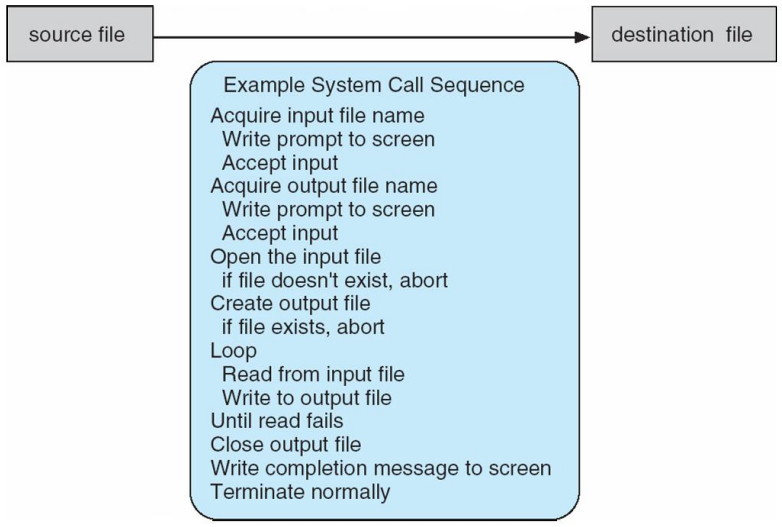
\includegraphics[width=0.6\linewidth]{img/image.png}    
    
\end{figure}

Example of API:

% \begin{lstlisting}[language=c]
% #include<unistd.h>

% ssize_t read(int fd, void *buf, size_t count)

% \end{lstlisting}

\begin{codeInC}
#include<unistd.h>
ssize_t read(int fd, void *buf, size_t count)
\end{codeInC}

\paragraph{}

But why do not programmers call the operating system call themselves instead of calling the library function?


The answar is \textbf{portability}. Programmer do not care about the implementation and the name of OS-call. So we shift the problems to the libraries. Different libraries (for different OS) implement the right system call.

Another answar is \textbf{Error}. If i call an OS-call with different type, e.g. an  integer instead of character parameter, I bother the OS and the CPU because OS throw an error.
Although if I call a function inside the program language library, it checks if all is right and forwards the request to the OS. 

\newpage
\subsubsection{API and OS Security}

\begin{figure}[htbp]
    \centering
    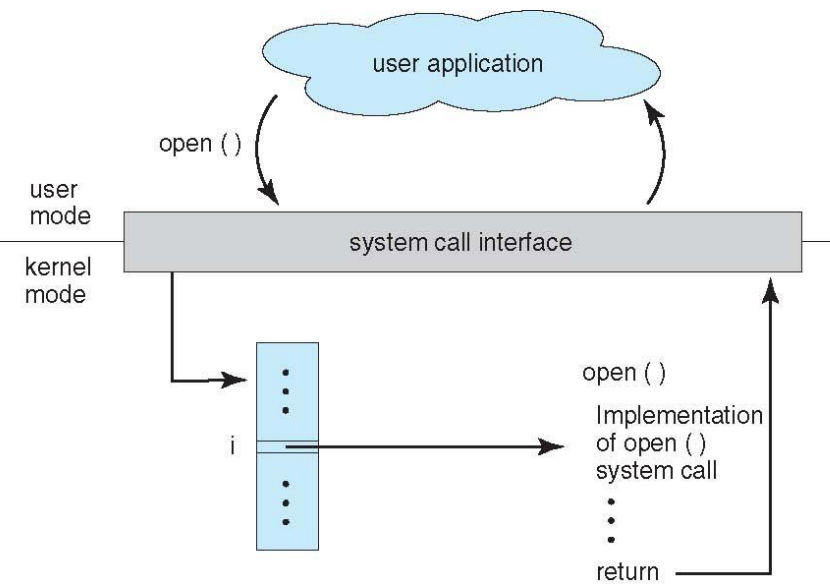
\includegraphics[width=0.6\linewidth]{img/API.png}
\end{figure}


\subsection{System call parameter passing}

There are three way to pass the parameters to OS-call:
\paragraph{}
-- The \textbf{firth}, the easiest way, is to copy all parameters into the registers but not always this method works. Normally the registers are less then the parameters.

\paragraph{}
-- The \textbf{second} way is to copy all parameters into a table or block and storing it in the ram and loading on register address of the cell where parameters are located.

This approach is used by Linux and Solaris OS.

\paragraph{}
-- The \textbf{last} approach is: Parameters placed, or pushed, onto the stack by the program
and popped off the stack by the operating system.


\begin{figure}[htbp]
    \centering
    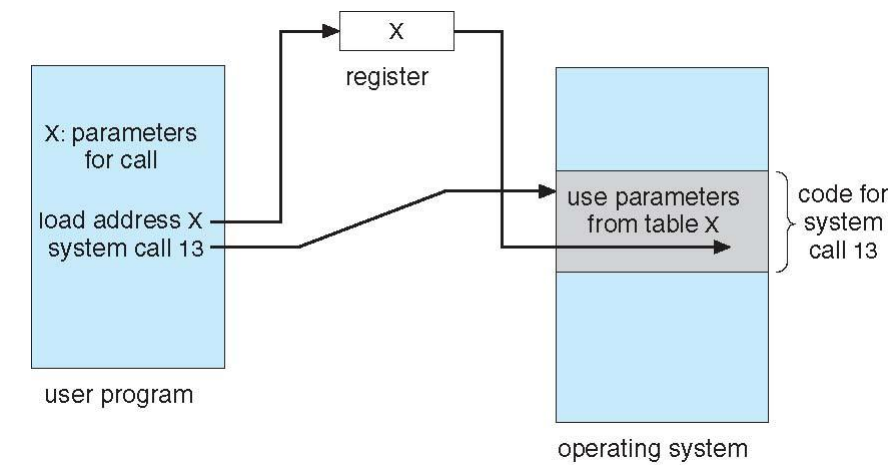
\includegraphics[width=0.6\linewidth]{img/params.png}
\end{figure}


\newpage
\subsection{Types of system call}

\begin{itemize} 

\item Process control
     \begin{itemize} 
        \item create process, terminate process
        \item end, abort
        \item load, execute
        \item wait for time
        \item wait event, signal event        
     \end{itemize}
     
\item File management
     \begin{itemize} 
        \item open, close
        \item create file, delete file
        \item read, write, append      
     \end{itemize}

\item Device management
     \begin{itemize} 
        \item read, write, reposition
        \item request device, release device
        \item logically attach or detach devices   
     \end{itemize}

\item Information maintenance
     \begin{itemize} 
        \item get time or date, set time or date
        \item get system data, set system data
     \end{itemize}

\item Communications
     \begin{itemize} 
        \item create, delete communication connection
        \item Shared-memory
        \item transfer status information
     \end{itemize}

\item Protection
     \begin{itemize} 
        \item Control access to resources
        \item Get and set permissions
        \item Allow and deny user access
     \end{itemize}
\end{itemize}



\begin{figure}[htbp]
    \begin{minipage}[htbp]{0.5\textwidth}
        \centering
        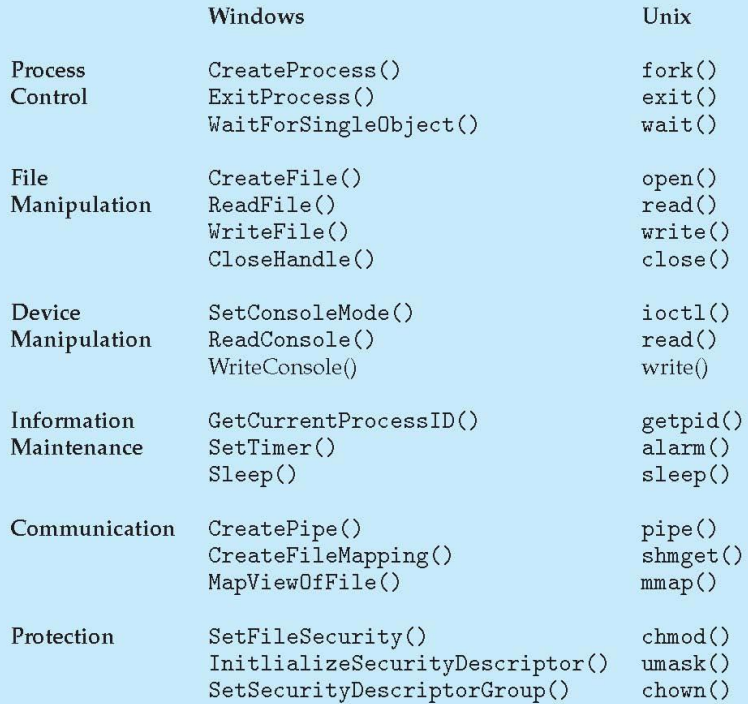
\includegraphics[width=0.9\linewidth]{img/SC.png}
    \caption{Windows and Unix System Call}
    \end{minipage}
    \begin{minipage}[htbp]{0.5\textwidth}
    \centering

    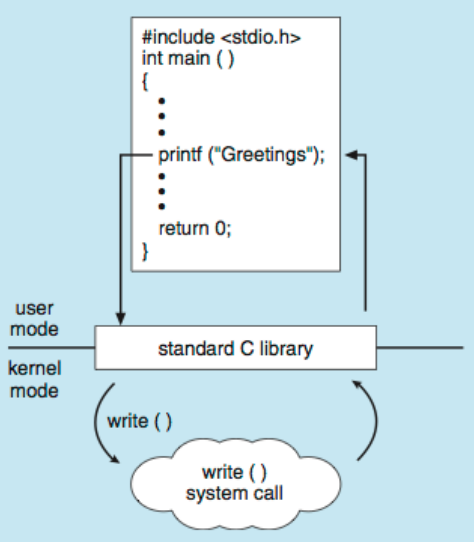
\includegraphics[width=0.8\linewidth]{img/print.png}
    \caption{Standard C library}       
    \end{minipage}
\end{figure}


\newpage
\subsection{MS-DOS}

The first OS (1982-2000) can run only single program, to open new program user must reload shell.

\subsection{FreeBSD}

First multitasking OS. Shell can open more then one program at the same time.

\section{Operating System Design and Implementation}
There aren't the best way to create an OS, it depends to different things:

\begin{itemize}
    \item HW
    \item SW
    \item Updating
    \item Usability...
\end{itemize}

\begin{itemize}
    \item \textbf{User Goals: }easy to learn, reliable, safe and fast.
    \item \textbf{System goals: }operating system should be easy to design, implement, and maintain, as well as flexible, reliable, error-free, and efficient
\end{itemize}

\paragraph{}
Some of this things conflict with the each other. GUI is more user-friendly but is more complex to implement GUI instead of CLI.

Some important principle to separate:

\begin{itemize}
    \item Policy: What will be done? policies decide what will be done

    \item Mechanism: How to do it? Mechanisms determine how to do something
\end{itemize}

\textbf{Example: }
\begin{itemize}
    \item[] Problem: exercising many processes
    \item[] Mechanism: Scheduling
    \item[] Policy: processes that use disk first, processes from a given user first, daemons first
\end{itemize}

\newpage
\section{Different kernel implementation}
There are different approach to implement the kernel in modern operating system; let's have a look of most of them.

\subsection{Monolithic Kernel - UNIX}
Original UNIX Kernel had a monolithic kernel structure splitted in two parts:

\begin{itemize}
    \item System programs
    \item The Kernel: Consists of everything below the OS-call interface and above the physical HW. Also it provides file system, other OS-function.
\end{itemize}

-- The pro of this approach: fast and energy efficient.

-- The cons: is not modulable, thus even small update requires recompilation from scratch and re-installation; no option to customize
\paragraph{}
This approach is the most used for OS kernel: linux use it and also android.




\subsection{Layered Approach}
OS is divided into a number of layers each with specific task built on top of lower layers. 

The \textbf{bottom} layer is the HW. The highest is the user interface.



This is more modular than monolithic approach. If you want to add or update some function in N-layer you just do it and recompile only N-layer and not all kernel.

Another aspect of this method, that remember TCP/IP stack, is that each level can only communicate with the lower level. 

\begin{figure}[htbp]
    \centering
    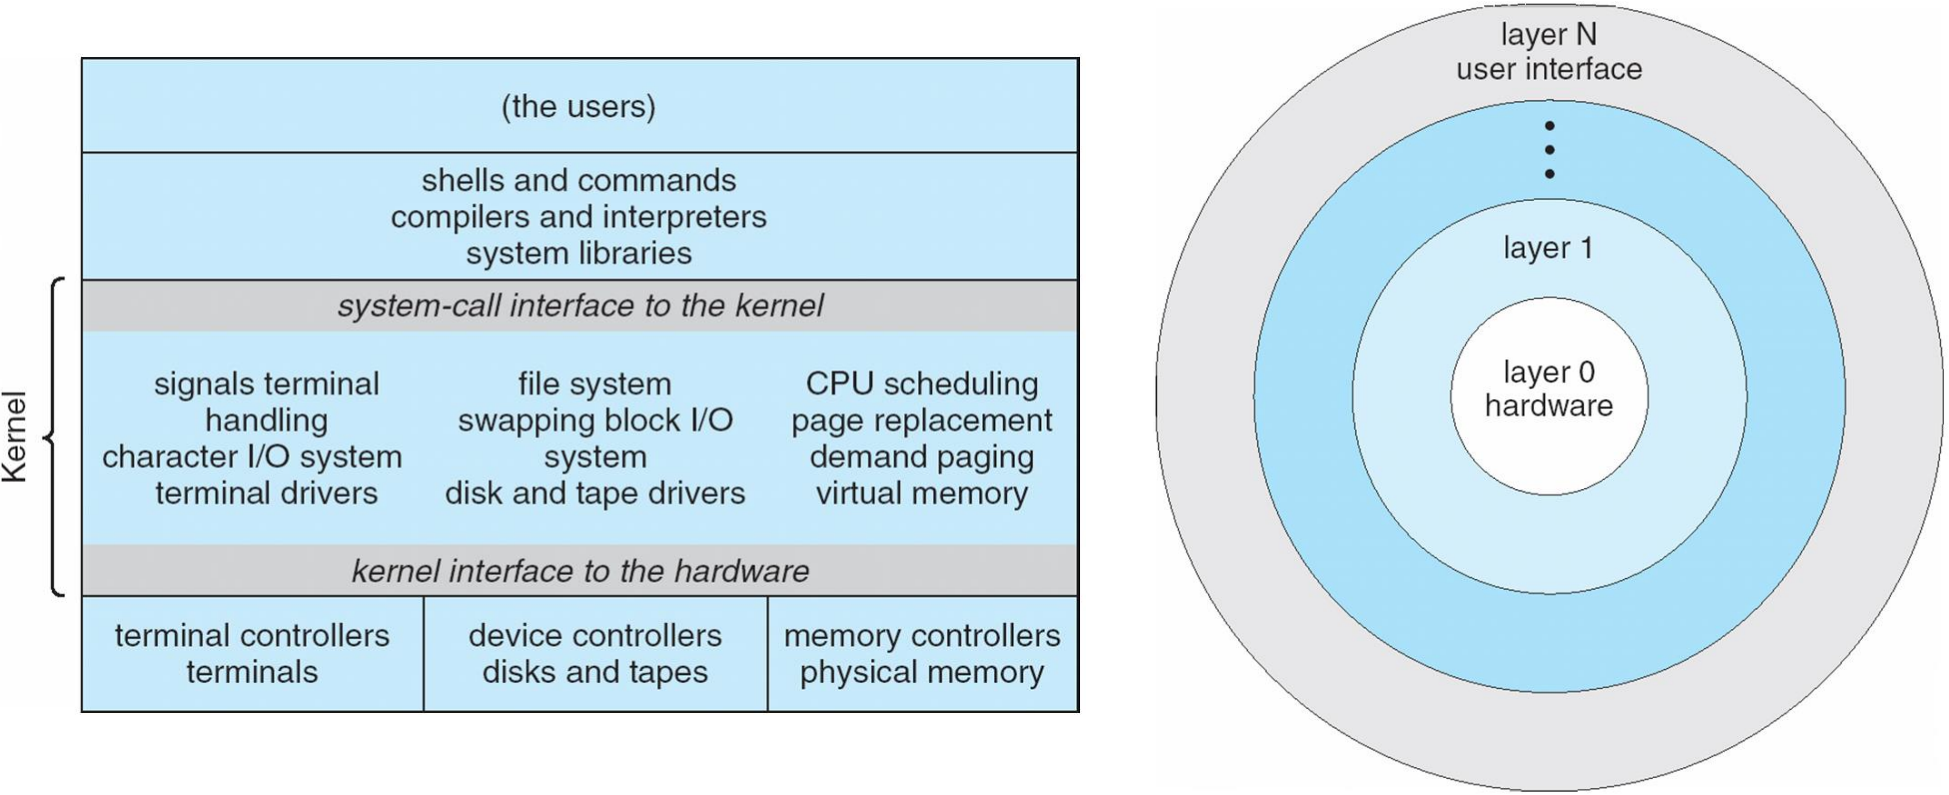
\includegraphics[width=0.85\linewidth]{img/kernel_mono_layer.png}
    \caption{Monolithic kernel left, Layered kernel right}
    
\end{figure}


\newpage
\subsection{MicroKernel System Structure}
MicroKernel is the tecnique that allow the most modular kernel. \textbf{Mach} is a particular example of microkernel, Max OS X kernel (Darwind) is based on Mach.

Obviously ther are pro and cons:
\paragraph{Pro:}
Easy to extend (best \textbf{modulability}); \textbf{portability} from OS to another with new architectures; \textbf{reliable} less cose running in kernel mode; \textbf{secure} malicious users process cant damage others.


\paragraph{Cons:}
Worst performance, lots of overhead is not direct communication because app must send a message to basic function of kernel.

\begin{figure}[htbp]
    \centering
    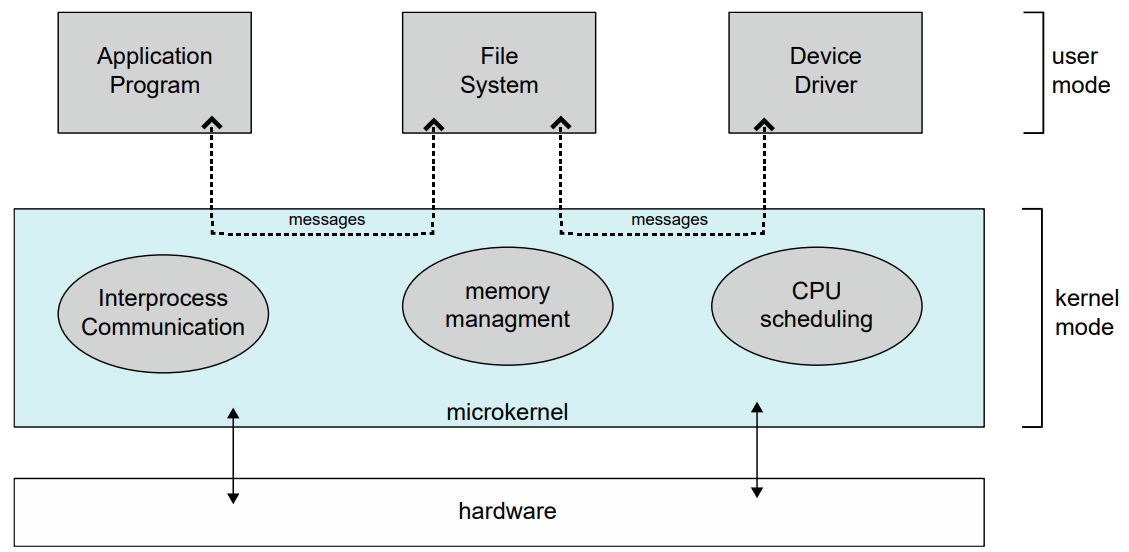
\includegraphics[width=0.6\linewidth]{img/microKer.png}
    \caption{micro kernel}
\end{figure}

\subsection{Solaris Modular Approach}
Solaris is OS used in business and/or commercial area that heavily use Oracle applications (Oracle DB, Java).

\subsection{Hybrid System}
Modern OS is a blended of monolithic, layer and microkernel features.
For example Windows is mostly monolithic but also it use microkernel structure. Also Mac OS X and Linux have a mix of different kernel structure.


\begin{figure}[htbp]
    \centering
    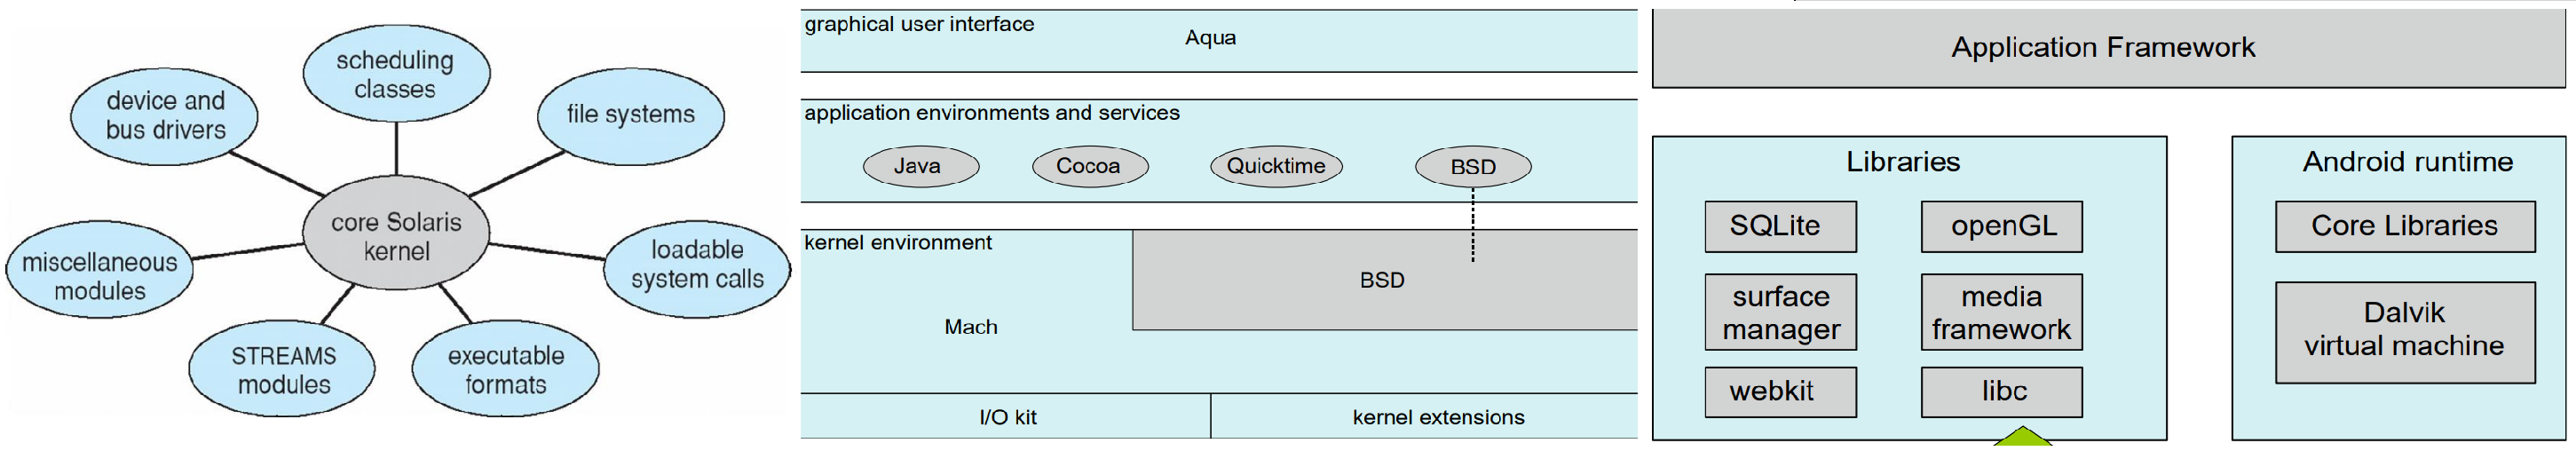
\includegraphics[width=1\linewidth]{img/kernel_3.png}
    \caption{Solaris left; Mac OS X center; Android right}
    
\end{figure}
\chapter{Process}

\section{Process Concept}

\textbf{Process} is a program in execution. Process execution must progress in sequential fashion, there are not parallel execution of instructions of a single process. 
\paragraph{}
Program is \textbf{passive} entity stored on disk (executable file), process is \textbf{active} so program becomes process when an executable file is loaded into memory.

One program can be has several process, think about multiple users executing.

\paragraph{}
An OS executes a variety of programs:
\begin{itemize}
    \item Batch system – jobs
    \item Time-shared systems – user programs or tasks
\end{itemize}

\paragraph{}
Process has multiple parts:
\begin{itemize}
    \item The program code, called text section
    \item Current activity including PC, processor register
    \item Stack containing temporary data (function params, return addresses, local variables)
    \item Data section containing global variables
    \item heap containing memory dynamically allocated during run time
\end{itemize}

\subsubsection{Memory layout of a C program}

\begin{figure}[htbp]
    \centering
    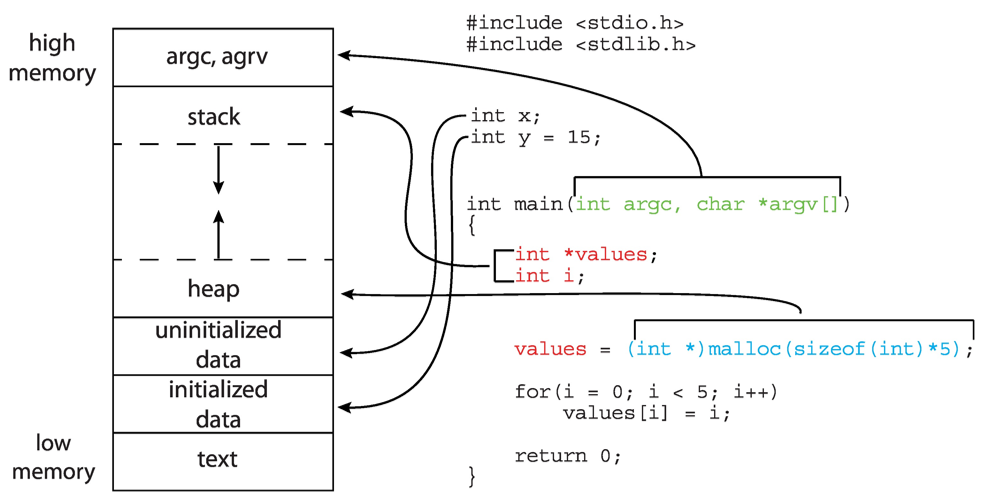
\includegraphics[width=0.7\linewidth]{img/memory_c_program.png}
    \caption{Relation to C program and memory usage}    
\end{figure}

We see that the heap grows upwards and the stack vice versa, this structure is used for efficiency. 

\subsection{Process State}
Process during this life change it states:

\begin{itemize}
    \item \textbf{New:} The process is being created
    \item \textbf{Ready:} The process is waiting to be assigned to a processor
    \item \textbf{Running:} Instruction are being executed
    \item \textbf{Waiting:} Process waiting for some event to occur (mouse click, I/O, interrupt)    
    \item \textbf{Terminated:} The process has finished execution
\end{itemize}


\begin{figure}[htbp]
    \centering
    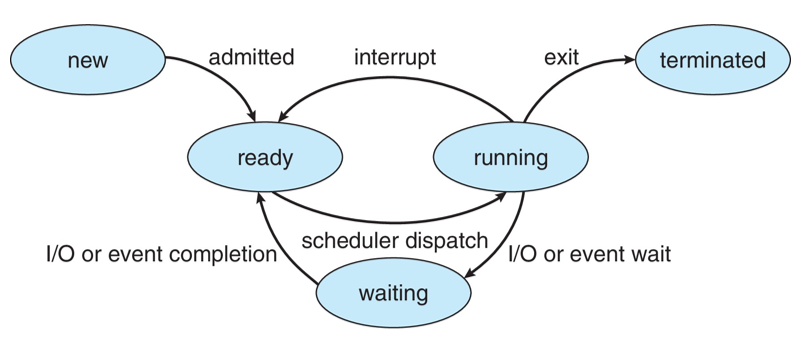
\includegraphics[width=0.6\linewidth]{img/process_state_diagram.png}
    \caption{Diagram of Process State}    
\end{figure}

\section{Process Control Block (PCB)}
All process must have information about the state, this block of information is called PCB and contains:

\begin{itemize}
    \item Process state - running, waiting...
    \item Program counter - location to the next code to execute
    \item CPU register 
    \item CPU scheduling info - priorities, scheduling queue
    \item Memory-management info - memory allocated to the process
    \item Accounting info - CPU usage, time since start, time limits
    \item I/O status info - list of open files
\end{itemize}

All of this information are used because when i resume the process i want the same data loaded into register and cache.

\begin{figure}[htbp]
    \centering
    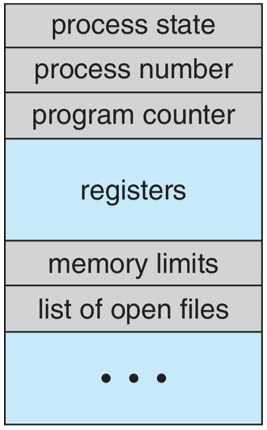
\includegraphics[width=0.17\linewidth]{img/PCB.png}
    \caption{Process Control Block (PCB)}    
\end{figure}

In Ubuntu we see PCBs in the folder: \verb|cat /proc/self/status| in this way we see the PCB of cat call, if we replace self with 1 (PID), we see the PCB of systemd.
Or using top command to see all Process ID.



\subsection{Context Switching}

When process require to wait, CPU stops to work on it an pass to another task. When CPU switch to another process, the system must save the state of the old process and load the salved state for the new process via \textbf{context switch}. The context is represented in the PCB.

Context switching time is pure overhead; the system does no useful work while switching, it is just a waste of time. More complex are OS and PCB and more longer context switch.

\section{Threads}
First of all threads are different from process, because if P1 run only one task it is a single thread process, otherwise is P1 run more tasks it becomes multi-thread process.
\paragraph{}
So far, a process has a single "script" of function, but now I want to code a program to execute in parallel to implement parallel search ecc. 

How can I do it?
\paragraph{}
Each thread has a PC assigned, thus a process has multiple program counter (Multiple locations can execute at once).

\begin{figure}[htbp]
    \centering
    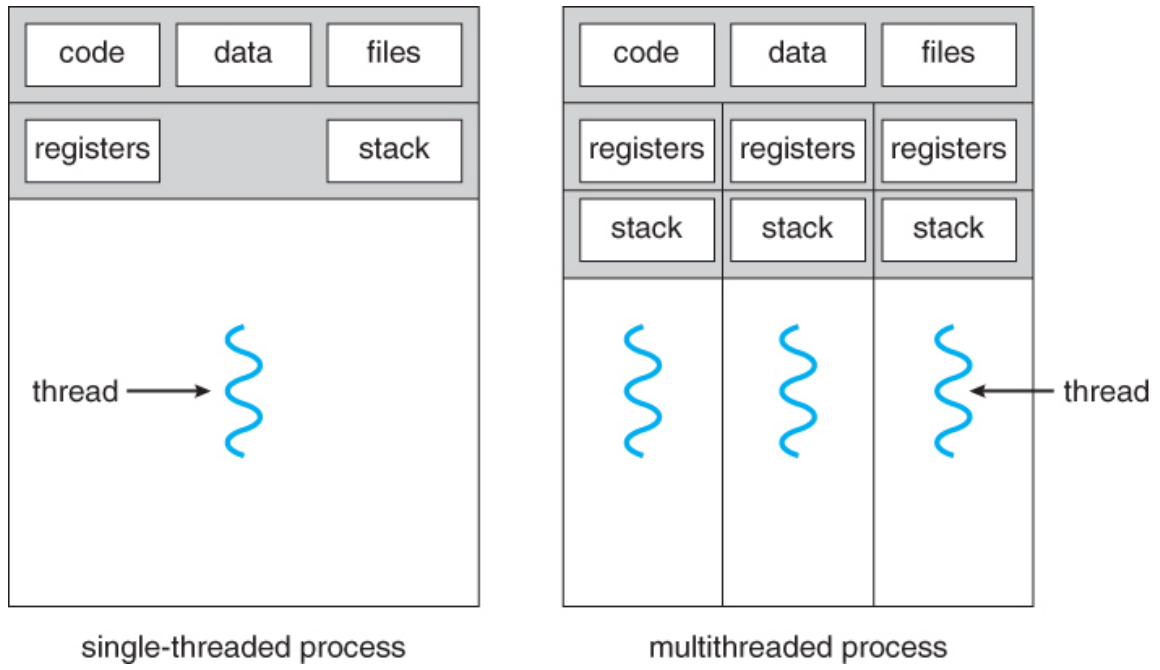
\includegraphics[width=0.5\linewidth]{img/thread.png}    
\end{figure}


\subsection{Multitasking in Mobile System}
Some mobile systems (e.g., early version of iOS)  allow only one process to run, others suspended.

\paragraph{IOS:}

\begin{itemize}
    \item Single foreground process- controlled via user interface
    \item Multiple background processes– in memory, running, but not on the display, and with limits
    \item Limits include single, short task, receiving notification of events, specific long-running tasks like audio playback

\end{itemize}


\paragraph{Android runs foreground and background, with fewre limits:}

\begin{itemize}
    \item Background process uses a service to perform tasks
    \item Service can keep running even if background process is suspended
    \item Service has no user interface, small memory use
\end{itemize}


\newpage
\section{Process Scheduling}

Process scheduler selects among available process for next execution on CPU core, the main goal of this process is to maximize the use of CPU, quickly switching onto CPU core.
Maintains updated two queue:

\begin{itemize}
    \item Ready queue: for all process that are ready to being execute
    \item Wait queues: for process that wait for some events (I/O)
\end{itemize}
Process normally migrate from one queue to the other.

\begin{figure}[htbp]
    \centering
    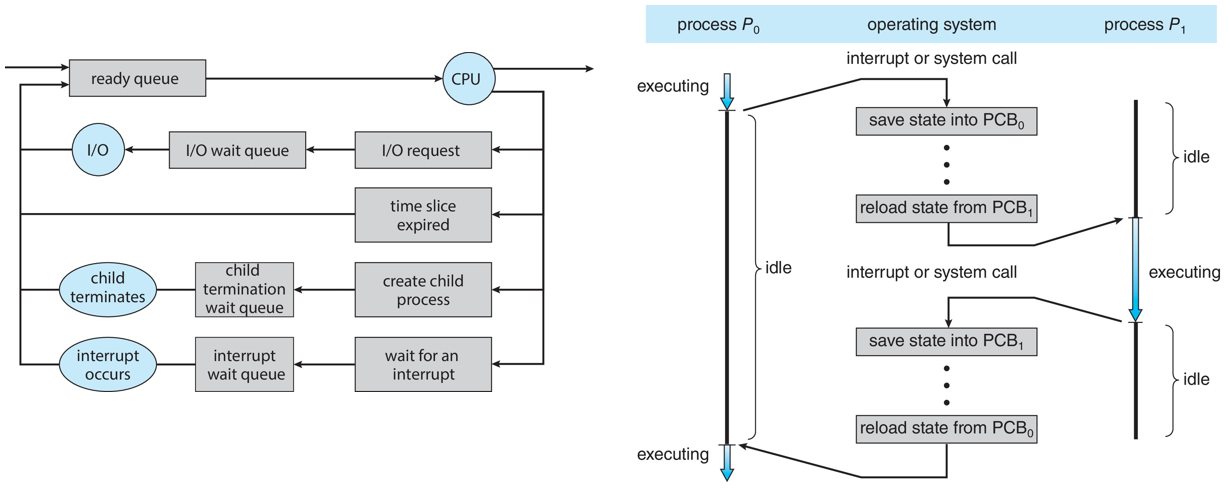
\includegraphics[width=0.95\linewidth]{img/scheduling.png}
    \caption{Process scheduling left; CPU switching right}    
\end{figure}



\section{Process Creation: }
Parent process create children process, witch can create other processes, forming a tree of processes.

Each process is \textbf{identified} by a process identifier: \textbf{pid} and they also has \textbf{resources} that could be shared by sharing option:

\begin{itemize}
    \item Parent and children share all resources
    \item Children share subset of parent's resources, like C++ Inheritance
    \item Parent and child share no resources
\end{itemize}

Processes can decide how to \textbf{execute}: parent and children execute concurrently or parent waits until children terminate.

Address space: 
\begin{itemize}
    \item Child duplicate of parent
    \item Child has a program loaded into it
\end{itemize}

\paragraph{UNIX example of OS-call:}
\begin{itemize}
    \item \textbf{fork()} : to create new process, return a $pid_t$ of children created
    \item \textbf{exec()} : used after fork() to replace the process' memory space with new program
    \item \textbf{wait()} : used by parent to waiting for the child to terminate.
\end{itemize}


\begin{figure}[htbp]
    \centering
    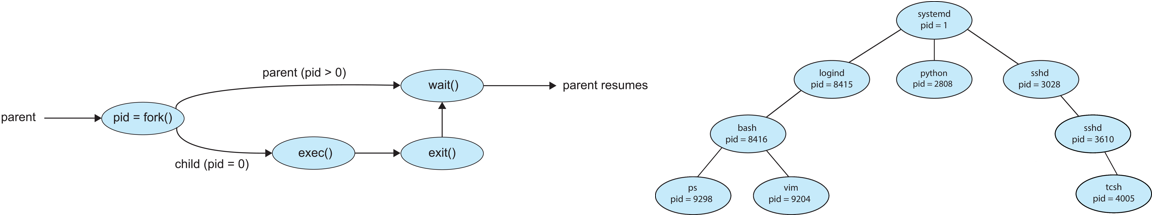
\includegraphics[width=1\linewidth]{img/process.png}
    \caption{OS-call left; process tree in Linux, \textit{pstree command}}    
\end{figure}


\subsubsection{C program forking separate process}
\begin{codeInC}
#include <sys/types.h>
#include <stdio.h>
#include <unistd.h>

int main() {

  pid_t pid;

  /* fork a child process */
  pid = fork();

  if (pid < 0) { /* error occurred */
    fprintf(stderr, "Fork Failed");
    return 1;
  } else if (pid == 0) { /* child process */
    execlp("/bin/ls", "ls", NULL);

  } else { /* parent process */

    /* parent will wait for the child to complete */
    wait(NULL);
    printf("Child Complete");
  }  

  return 0;
}

\end{codeInC}


\newpage
\section{Process termination}

Each process can decide to terminate the task at any time. Process usually executes last statement and than asks to the OS to delete it using \textbf{ exit()} call.

All children's status returns to parent (via \textbf{wait()} call) and process' resources are deallocated by OS.

In some cases parent can use the \textbf{abort()} call to terminate the execution of children. Some reasons of doing it:

\begin{itemize}
    \item Children has exceeded allocated resources
    \item The task assigned to children is no longer required
    \item OS call exit() call to the parent process and children must terminate to do the assigned task because OS does not allow to continue if its parent terminates.
\end{itemize}

Some OS wait until all the process terminates' children terminates, it called cascading termination.
The parent process may wait for termination of a child process by using \textbf{wait() syscall}. The call returns status, information and pid of the terminated process.

\begin{codeInC}
pid  = wait(&status);
\end{codeInC}

If no parent waiting (did not invoke wait()) process is a \textbf{zombie}.

If parent terminated without invoking wait(), process is an \textbf{orphan}.



\section{Android process termination importance hierarchy}
All mobile smartphones have limited resources such as memory compare to PCs. Thus, the android OS has to manage process termination to improve performance. Below there is a list of process, from most to least important: 

\begin{itemize}
    \item Foreground process;
    \item Visible process;
    \item Service process;
    \item Background process;
    \item Empty process;
\end{itemize}

Android terminates less important processes weed out unused memory. 

\section{Inter-process Communication}

Process within a system may be \textbf{independent} or \textbf{cooperating}.
Cooperating process can affect or be affected by other processes, including sharing data.

Cooperating processes need \textbf{interprocess communication} \textbf{IPC}, obviously there are reasons for cooperating process:

\begin{itemize}
    \item information sharing;
    \item computation speedup;
    \item modularity;
    \item convenience;
\end{itemize}

\paragraph{}
Also there are two different way to implement IPC: 
\begin{itemize}
    \item Shared memory: you define a specific space into ram where two process can access and communicate
    \item Message passing
\end{itemize}

\begin{figure}[htbp]
    \centering
    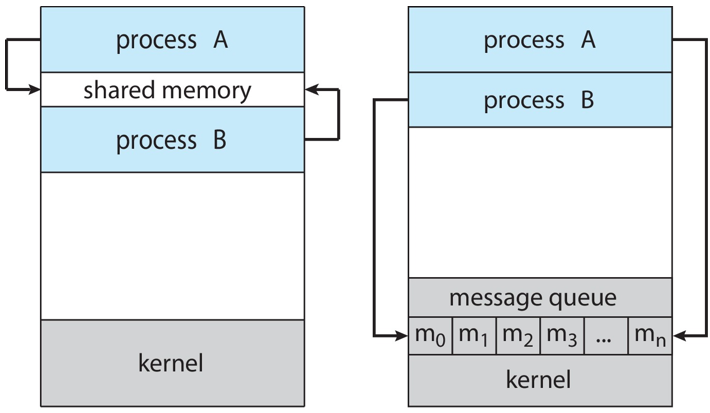
\includegraphics[width=0.5\linewidth]{img/IPC.png}
    \caption{shared memory left; message passing right}    
\end{figure}

\subsection{Producer-consumer problem}

Producer process produces information that is consumed by consumer process, two variations:

\begin{itemize}
    \item unbounded-buffer places no practical limit on the size of buffer:
    \begin{itemize}
        \item[] Producer never waits
        \item[] consumer waits if there is no buffer to consume
    \end{itemize}

    \item bounded-buffer assumes that there is a fixed buffer size:
    \begin{itemize}
        \item[] Producer must wait if all buffer are full
        \item[] Consumer waits if there is no buffer to consume
    \end{itemize}
\end{itemize}

 \subsection{IPC - Message Passing}
Major issues is to provide mechanism that will allow the user processes to synchronize their actions when they access shared memory.

\subsubsection{Example of IPC - POSIX}
POSIX Shared Memory: Process P1 create shared memory segment, an area of RAM memory.

\begin{codeInC}
shm_fd = shm_open(name, O CREAT | O RDWR, 0666);
\end{codeInC}

and set the size of the existing segment:
\begin{codeInC}
ftruncate(shm_fd, 4096); 
\end{codeInC}

In this way you create an area of memory and you must use it like a file, calling the default call for file descriptor: open, read, write, close, seek...

\newpage
\subsubsection{Memory-map}
If you use the function \textit{mmap()}, you transform the file in array of bytes. You just modified the access to the byets not the content. Using this method you also can access to virtual memory a concept that we will see later.


\subsubsection{IPC POSIX Producer}
\begin{codeInC}
#include <stdio.h>
#include <stdlib.h>

#include <string.h>
#include <fcntl.h>

#include <sys/shm.h>
#include <sys/stat.h>

int main() {

    /* the size (in bytes) of shared memory object */
    const int SIZE = 4096;
    
    /* name of the shared memory object */
    const char *name = "OS";
    
    /* strings written to shared memory */
    const char *message0 = "Hello";
    const char *message1 = "World!";
    
    /* shared memory file descriptor */
    int shm_fd;
    
    /* pointer to shared memory object */
    void *ptr;
    
    /* create the shared memory object */
    shm_fd = shm_open(name, O_CREAT | O_RDWR, 0666);
    
    /* configure the size of the shared memory object */
    ftruncate(shm_fd, SIZE);
    
    /* memory map the shared memory object */
    ptr = mmap(0, SIZE, PROT_WRITE, MAP_SHARED, shm_fd, 0);
    
    /* write to the shared memory object */
    sprintf(ptr, "%s", message0);    
    ptr += strlen(message0);  // you must do it otherwise you rewrite the bytes
    sprintf(ptr, "%s", message1);
    ptr += strlen(message1);
    
    return 0;
}

\end{codeInC}

\newpage
\subsubsection{IPC POSIX Consumer}
\begin{codeInC}
#include <stdio.h>
#include <stdlib.h>

#include <fcntl.h>
#include <sys/shm.h>

#include <sys/stat.h>

int main() {

    /* the size (in bytes) of shared memory object */
    const int SIZE = 4096;
    
    /* name of the shared memory object */
    const char *name = "OS";
    
    /* shared memory file descriptor */
    int shm_fd;
    
    /* pointer to shared memory object */
    void *ptr;
    
    /* open the shared memory object */
    shm_fd = shm_open(name, O_RDONLY, 0666);
    
    /* memory map the shared memory object */
    ptr = mmap(0, SIZE, PROT_READ, MAP_SHARED, shm_fd, 0);
    
    /* read from the shared memory object */
    printf("%s", (char *)ptr);    
    
    /* remove the shared memory object */
    shm_unlink(name);  //like close(), you free the memory to OS.
    
    return 0;
}

\end{codeInC}


The only way to get access the S.M. is to know the name of the shared memory object, so it must be \textbf{secret}.

\newpage
 \subsection{IPC - Message Passing}
 Processes communicate with each other without resorting to shared variables, thus IPC provide two option: \textbf{send} and \textbf{receive} massage. The size of message is fixed or variable.

 \paragraph{}
 If process \textit{P} and \textit{Q} wish to communicate, they need:
 \begin{itemize}
     \item Establish a communication link between them
     \item Exchange messages via send and receive
 \end{itemize}
 
\paragraph{How to implement this communication?} How to establish the link? The link is connected with one ore more processes? Capacity of the link? 

\subsection{Direct Communication}
Processes must name each other explicitly:

\begin{itemize}
    \item send(P, msg) - send a message to process P
    \item receive(Q, msg) - receive a message from process Q
\end{itemize}

The proprieties of communication link are: links are established automatically, bi-directional and between each pair exist only one link.

\subsection{Indirect communication}

Indirect communication is different as Direct communication because it uses a mailbox to communicate.


Each mailbox has a unique id and process can communicate only if they share a mailbox.

The proprieties of communication link are: links are established only if processes share a common mailbox, link could be associated with several processes and each process may share several communication links, links may be unidirectional or bi-directional.

\begin{itemize}
    \item send(A, msg) - send a message to mailbox A
    \item receive(A, msg) - receive a message from mailbox A
\end{itemize}

In this way there is a problem. If P1, P2 and P3 share mailbox A and P1 send a message, who receive the message?

\paragraph{Some solutions could be:}
\begin{itemize}
    \item Create link associated only a two processes (like direct communication)
    \item  Allow only one process at a time to execute a receive operation
    \item Allow the system to select arbitrarily the receiver
\end{itemize}

\newpage
\subsection{Synchronization}
The messages could be blocking or non-blocking message:


\paragraph{Blocking} is considered synchronous
\begin{itemize}
    \item \textbf{Blocking send} - the sender is blocked until the message is received
    \item \textbf{Blocking receive} - the receiver is blocked until the message is available
\end{itemize}

\paragraph{Non-blocking} is considered asynchronous
\begin{itemize}
    \item \textbf{Non-blocking send} - the sender sends the message and continue
    \item \textbf{Non-blocking receive} - the receiver receives a valid message or null message
\end{itemize}

Different combinations are possible but if both, sender and receiver, are blocked we have a \textbf{rendezvous}.

\subsection{IPC Systems - Windows}

The message passing in Windows pass throw \textbf{advanced local procedure call}: 
\begin{itemize}
    \item Only works between processes on the same system
    \item Uses ports (like mailbox) to established and maintain communication link
\end{itemize}

Communication works as follows:

\begin{enumerate}
    \item The client open a handle to the subsystem's connection port object
    \item the client sends a connection request
    \item the server create two private communication ports and return the handle to the client
    \item the client and server use corresponding port handle to send messages and/or callback a to listen for replies
\end{enumerate}

\begin{figure}[htbp]
    \centering
    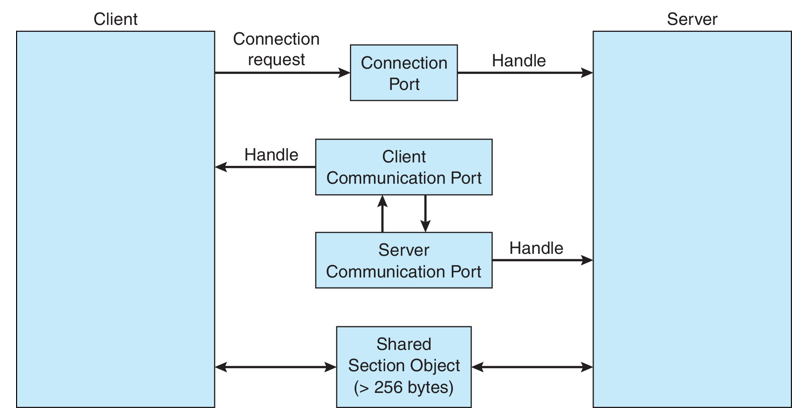
\includegraphics[width=0.65\linewidth]{img/LPC.png}
    \caption{Message passing via advanced Local Call LPO}
    
\end{figure}

\newpage
\section{Pipes}
Pipes acts as a conduit allowing to processes to communicate. There are some issues like: are uni or bi directional and in case of two-way communication it is half or full duplex?

There are two different type of pipes:

\begin{itemize}
    \item \textbf{Ordinary pipes} - the pipe cannot be accessed from outside the process that created it. Typical example might be: parent create a process and want to communicate with child that it created.
    \item \textbf{Named pipes} - can be accessed without a parent-child relationship
\end{itemize}

To create a pipe you must call the \textit{mkfifo("name", 0666)}

\subsection{Ordinary pipes}
This ordinary pipe allow to communicate only if you have a parent-child relationship.

Producer write in one end (write-end) and the consumer read from the another end (read-end). Ordinary pipes are therefore unidirectional.

\begin{figure}[htbp]
    \centering
    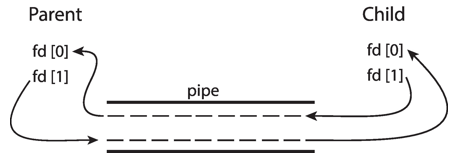
\includegraphics[width=0.55\linewidth]{img/O_Pipes.png}
    \caption{Ordinary pipes}    
\end{figure}

Windows calls this pipe \textbf{anonymous pipes}.

\newpage
\subsubsection{Ordinary UNIX pipes}
\begin{codeInC}
#include <stdio.h>
#include <unistd.h>
#include <sys/types.h>
#include <string.h>

#define BUFFER_SIZE 25
#define READ_END	0
#define WRITE_END	1

int main(void){
	char write_msg[BUFFER_SIZE] = "Greetings";
	char read_msg[BUFFER_SIZE];
	pid_t pid;
	int fd[2];

	/* create the pipe */
	if (pipe(fd) == -1) {
		fprintf(stderr,"Pipe failed");
		return 1;
	}

	/* now fork a child process */
	pid = fork();

	if (pid < 0) {
		fprintf(stderr, "Fork failed");
		return 1;
	}

	if (pid > 0) {  /* parent process */
		/* close the unused end of the pipe */
		close(fd[READ_END]);

		/* write to the pipe */
		write(fd[WRITE_END], write_msg, strlen(write_msg)+1); 

		/* close the write end of the pipe */
		close(fd[WRITE_END]);
	}
	else { /* child process */
		/* close the unused end of the pipe */
		close(fd[WRITE_END]);

		/* read from the pipe */
		read(fd[READ_END], read_msg, BUFFER_SIZE);
		printf("child read %s\n",read_msg);

		/* close the write end of the pipe */
		close(fd[READ_END]);
	}
	return 0;
}

\end{codeInC}

\newpage
\subsection{Named pipes}

This pipes are more powerful than the ordinary pipes, indeed communication is bidirectional; no parent-child relationship is necessary; several processes can use the named pipe for communication.

This type of pipes are provided on both UNIX and Windows systems.

\subsubsection{Named UNIX Pipe read}
\begin{codeInC}
#include <sys/types.h>
#include <sys/stat.h>
#include <fcntl.h>
#include <unistd.h>
#include <string.h>
#include <stdio.h>
#include <stdlib.h>

#define BUFFSIZE 512
#define err(mess) { fprintf(stderr,"Error: %s.", mess); exit(1); }

void main(){
    int fd, n;
    char buf[BUFFSIZE];

    if ( (fd = open("fifo_x", O_RDONLY)) < 0)
        err("open");
    while( (n = read(fd, buf, BUFFSIZE) ) > 0) {
        if ( write(STDOUT_FILENO, buf, n) != n) { 
            exit(1);
        }
    }
    close(fd);
}

\end{codeInC}

\subsubsection{Named UNIX Pipe write}
\begin{codeInC}
#include <sys/types.h>
#include <sys/stat.h>
#include <fcntl.h>
#include <unistd.h>
#include <string.h>
#include <stdio.h>
#include <stdlib.h>

#define BUFFSIZE 512
#define err(mess) { fprintf(stderr,"Error: %s.", mess); exit(1); }

void main(){
    int fd, n;
    char buf[BUFFSIZE];

    mkfifo("fifo_x", 0666);
    if ( (fd = open("fifo_x", O_WRONLY)) < 0)
        err("open");
    while( (n = read(STDIN_FILENO, buf, BUFFSIZE) ) > 0) {
        if ( write(fd, buf, n) != n) { 
            err("write");
        }
    }
    close(fd);
}

\end{codeInC}

\section{Communication in Client-Server Systems}

So far we have talked about the intern communication, now we want to communicate with other processes.
To talk about it we introduce the \textbf{Soket} system.

\subsection{Sockets}
A socket is defined as an endpoint for communication, concatenate IP address and port to the receiver: 192.168.1.1:80. 

All ports below 1024 are \textbf{well known} used for standard servicies like mail 25, secure web browsing 443, FTP 20 21 etc.

\subsection{Remote Procedure Calls}

The Remote Procedure Calls RPC abstracs procedures calls between processes on networked systems. Again it use ports for service differentiation.

Data are represented by \textbf{External Data Representation, XLD}, thus it can be read by different architecture: Big-endian and Little-endian.

\begin{figure}[htbp]
    \centering
    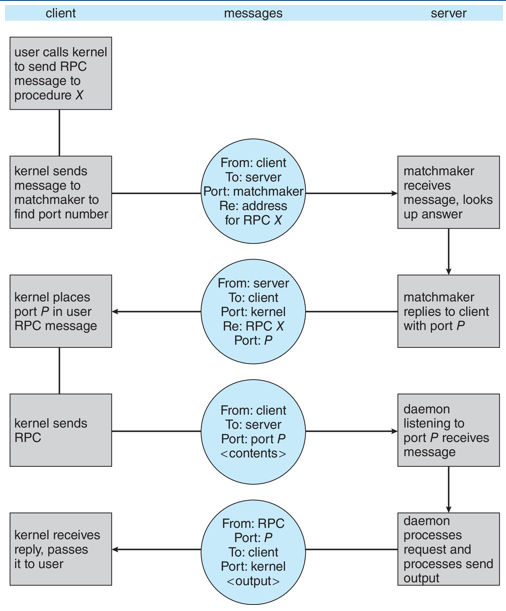
\includegraphics[width=0.7\linewidth]{img/RPC.png}
    \caption{Execution of RPC}
    
\end{figure}
\newpage
\chapter{Threads \& Concurrency}

\section{Process Concept}

Task, process and subprocess are all synonym. We talked about how to fork a process, parent con create a child a copy of the parent. They are two different process with one signle thread each.

We also sad that when we switch from process to another the context switch must copy all the data (registers, PC, code, opened files, etc.) and this require time and more small it is more efficient are the OS.

So is not efficient to duplicate all the parent instead of a small part of process.
\paragraph{}
We would like to reduce this overhead to improve overall performance and the solution is to use \textbf{thread}. 

\subsection{Motivation}

Most, may be all, modern application are multithreaded, thread run within application. Multiple tasks, in a single application, can be implemented by separated threads:
\begin{itemize}
    \item Update display;
    \item Fetch data from file/network;
    \item Spell checking;
    \item Send data into the net;
    \item etc.
\end{itemize}

Also they can simplify code and increase efficiency also kernel are generally multithreaded.
\paragraph{}
Another big difference is: process creation is \textbf{heavy-weight}, like I sad before, while thread creation is \textbf{light-weight}.

\newpage

\section{Multi-Threading}

\subsubsection{Single and Multithreaded processes}

\textbf{Thread} is a basic unit of CPU usage composed of \textbf{thrID}, \textbf{PC}, \textbf{register set}, \textbf{stack} and some shared data: \textbf{heap data}, \textbf{code} (text) and \textbf{OS resouces} with other threads belonging to the same process.

\begin{figure}[htbp]
    \centering
    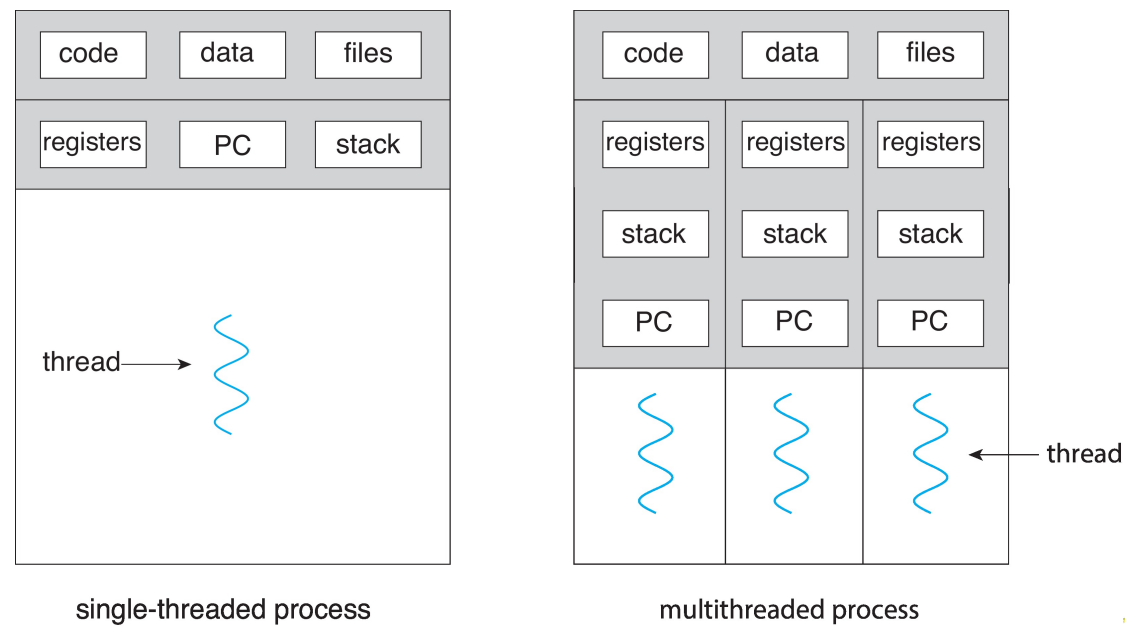
\includegraphics[width=0.65\linewidth]{img/threads.png}   
\end{figure}

Example:
\begin{figure}[htbp]
    \centering
    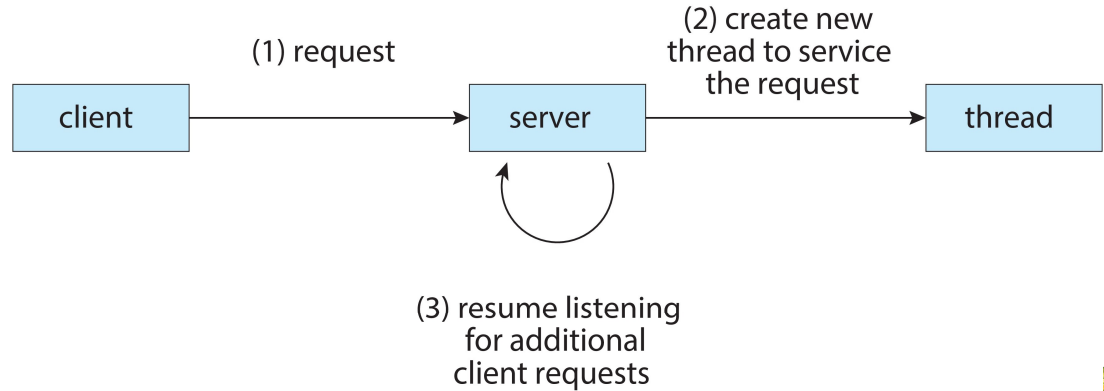
\includegraphics[width=0.65\linewidth]{img/thread_EX.png}   
    
\end{figure}



\subsection{Fork == Thread?}
At this point, you may ask yourselves if the UNIX fork spawns a \textbf{new process} (child of the caller) or a \textbf{Thread}? The answer is: it spawns a child process.

But then, what is the difference between a child process and a thread?

\subsection{Linux Threads}
For Linux systems refers to them as \textbf{tasks} rather than \textbf{threads}.

Task (process) creation is done through \textit{fork()} but also Task (thread) creation is done through \textit{clone()} system call. This function, depends on the parameters passed, can allows a child task to share the address spaces of the parent task (process).

Flags control behavior, can be used for both:

\begin{figure}[htbp]
    \centering
    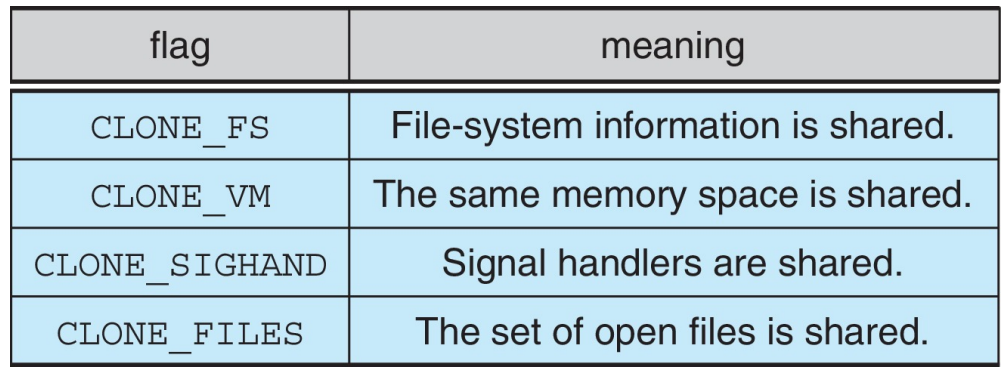
\includegraphics[width=0.55\linewidth]{img/flags.png}
    \caption{Flags to use in clone}    
\end{figure}

\newpage
By default:
\begin{itemize}
    \item fork copies all data structures of the parent process to the child,
    \item while clone points to them
\end{itemize}

\subsubsection{Fork child processes:}
Are processes, so its creation is heavier than threads, the purpose is to create a new process, which becomes the child
process of the caller. Both processes will execute the next instruction following the \textit{fork()} system call and if the child wants to communicate with the parent, it has to set-up brand new shared memories or message-passing because if the parents change the value of a variable the child does not see it (because is a copy).

Two identical copies of the computer's address space,code, and stack are created one for parent and child. Like "Dolly" sheep.


\subsubsection{Threads:}
Purpose is to create a new thread in the program which is given the same process of the caller and threads within the same process can communicate using
shared memory.

The second thread will share data, open files, signal handlers
and signal dispositions, current working directory, user and
group ID's. The new thread will get its own stack, thread ID,
and registers though.

Continuing the analogy: if it was a sheep, your process grows a
fifth head or a second tail when it creates a new thread; those are
connected and share the same brain.


\subsubsection{In my OS}

But then, is my OS scheduling processes or threads?

\begin{itemize}
    \item The Linux scheduler (on recent Linux kernels, e.g. 3.0 at least) is scheduling schedulable tasks or “ready” tasks. 
    \item A task/job may be: 
        \begin{itemize}
            \item[]a single-threaded process (e.g. the main of a C code, or something
created by fork without any thread library);
            \item[] any thread inside a multi-threaded process (including its main
thread), in particular Posix threads;
            \item[] kernel tasks, which are started internally in the kernel and stay in
kernel land (e.g. kworker, nfsiod, kjournald …). These are managed directly by the OS.
        \end{itemize}
\end{itemize}

In other words, threads inside multi-threaded processes are scheduled
like non-threaded -i.e. single threaded- processes.

\section{Benefits}
Using threads improve the overall OS this is some resons:
\begin{itemize}
    \item \textbf{Responsiveness} -- may allow continued execution if part of
    process is blocked, especially important for user interfaces;
    
    \item \textbf{Resource Sharing} -- threads share resources of process, easier
    than shared memory or message passing;
    
    \item \textbf{Economy} -- cheaper than process creation, thread switching
        lower overhead than context switching: \textbf{Don’t need to resent} the cache/CPU is I am switching from a
        process thread to another thread of the same process;
        
    \item \textbf{Scalability} -- process can take advantage of multicore
    architectures: This is true also for single-threaded processes if handled
correctly.
\end{itemize}

\newpage
\section{Multicore Programming}

Multicore or multiprocessor systems put pressure on programmers,
challenges include:

\begin{itemize}
    \item[] Dividing activities
    \item[] Balance load
    \item[] Data splitting
    \item[] Data dependency
    \item[] Testing and debugging
\end{itemize}


\paragraph{Concurrency: } supports more than one task making progress. Single processor / core, scheduler providing concurrency.
\begin{figure}[htbp]
    \centering
    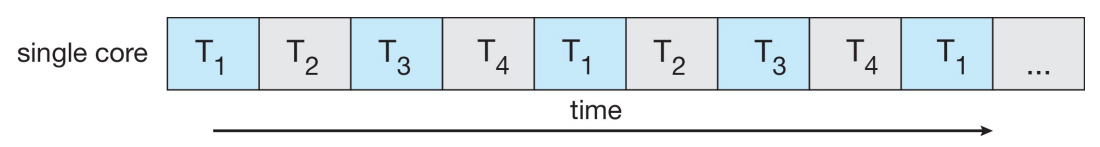
\includegraphics[width=0.7\linewidth]{img/CONCURRENT.png}
    \caption{Concurrent execution on single-core system}
    
\end{figure}
Not really concurrent, there is still at most a thread executing at once. However, it gives the impression that many things are running in
parallel.

If there are lots of process the time between the first and the last are more relevant.
\paragraph{}

\paragraph{Parallelism: } implies a system can perform more than one task simultaneously.

\begin{figure}[htbp]
    \centering
    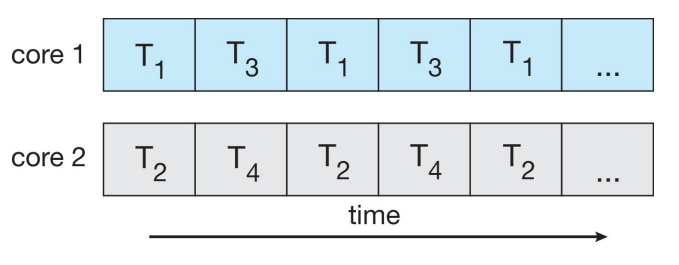
\includegraphics[width=0.45\linewidth]{parallel_exe.png}
    \caption{Parallel execution on a multi-core system}    
\end{figure}

The are two type of parallelism:

\begin{itemize}
    \item -- \textbf{Data parallelism:} distributes subsets of the same data
across multiple cores, same operation on each, none data is shared with other tasks;
        \begin{itemize}
            \item[] e.g. quicksort, margesort.
        \end{itemize}
    \item -- \textbf{Task parallelism:} distributing threads across cores, each
thread performing \textbf{unique operation}, you have some data that it can be shared in different tasks.
        \begin{itemize}
            \item[] e.g. pipelining
        \end{itemize}
\end{itemize}

\begin{figure}[htbp]
    \centering
    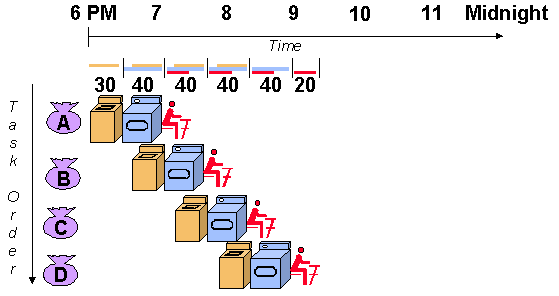
\includegraphics[width=0.65\linewidth]{img/pipeling.png}
    \caption{Pipelining}    
\end{figure}

\newpage
Pipelining, a standard feature in RISC processors, is much like an assembly line. Because the processor works on different steps of the instruction at the same time, more instructions can be executed in a shorter period of time.


\paragraph{RISC Pipelines:} A RISC processor pipeline operates in much the same way, although the stages in the pipeline are different. While different processors have different numbers of steps, they are basically variations of these five, used in the MIPS R3000 processor:

\begin{enumerate}
    \item fetch instructions from memory
    \item read registers and decode the instruction
    \item execute the instruction or calculate an address
    \item access an operand in data memory
    \item write the result into a register
\end{enumerate}

\begin{figure}[htbp]
    \centering
    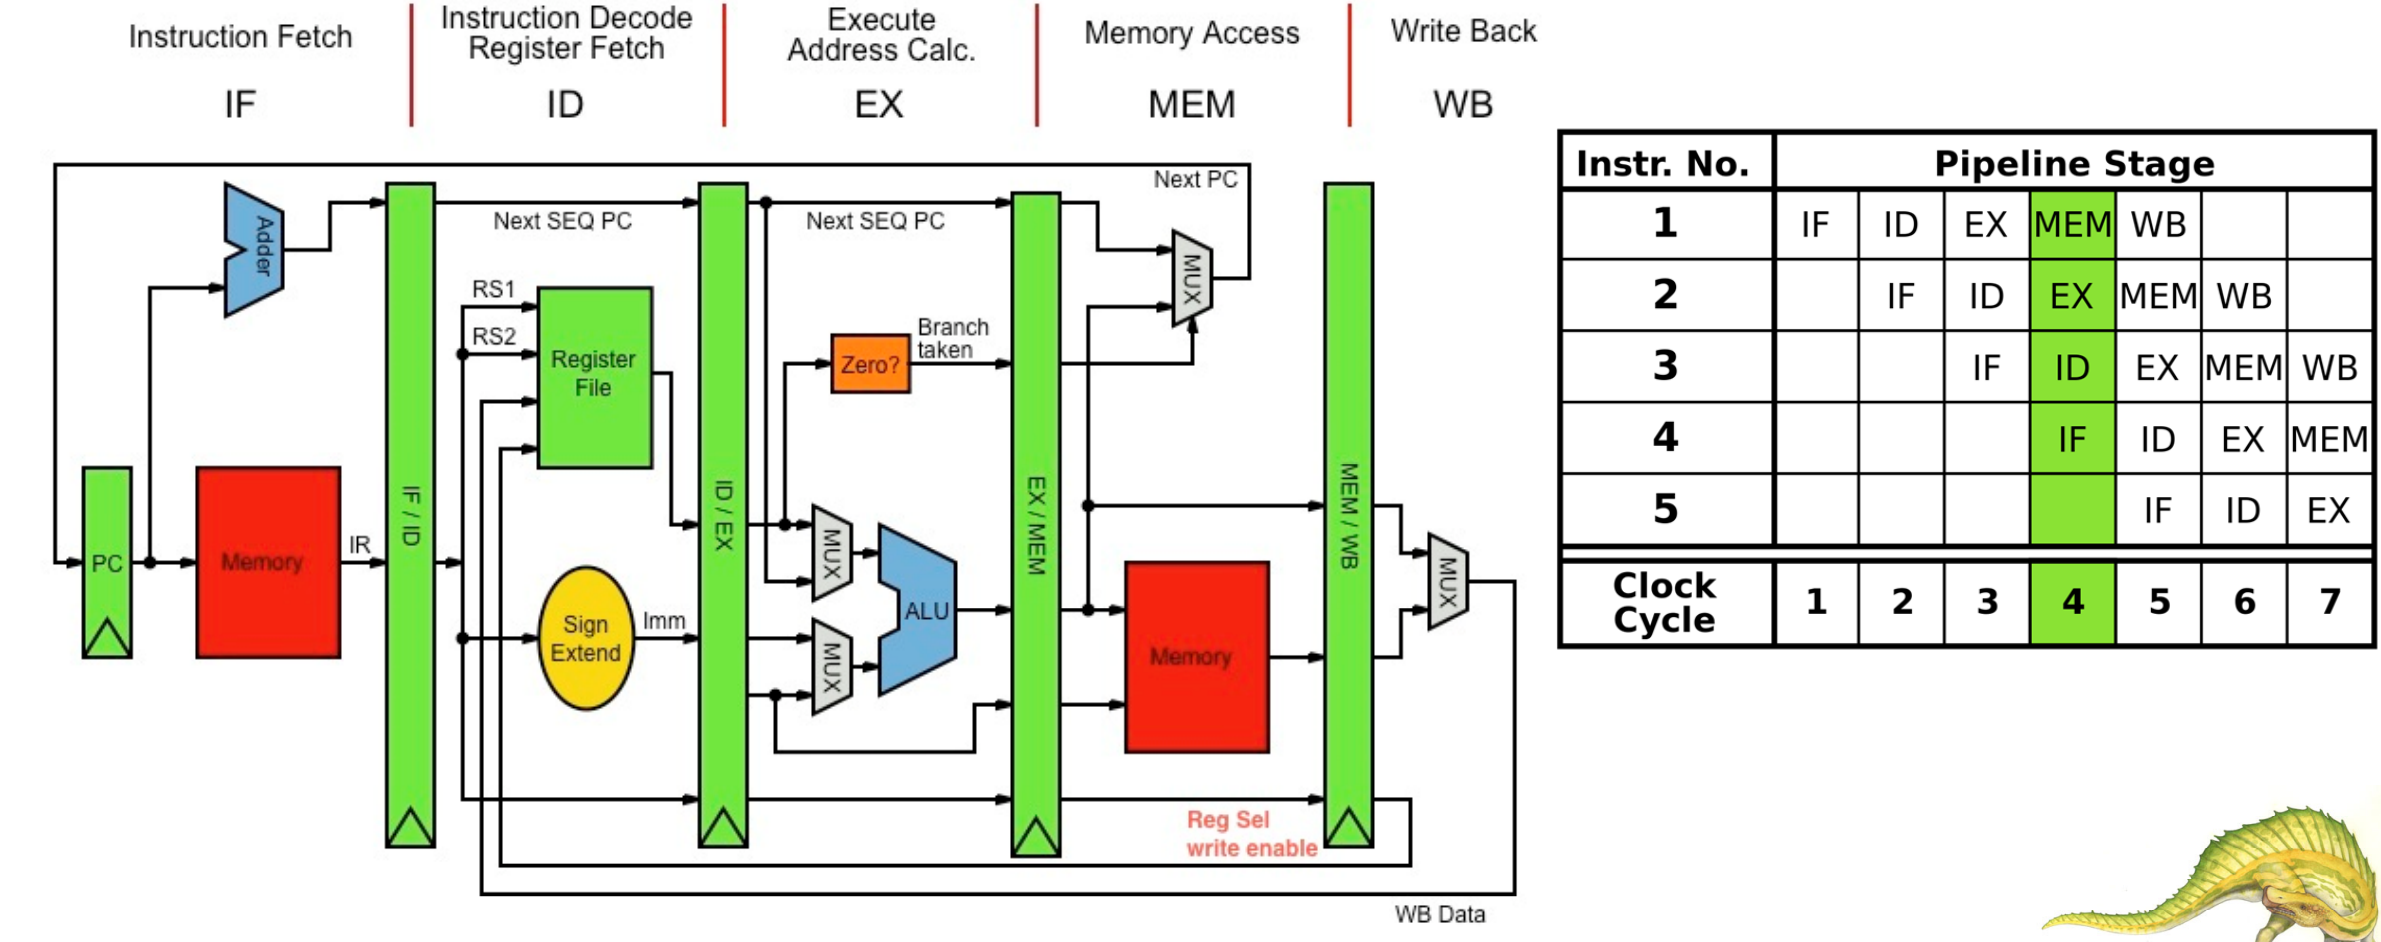
\includegraphics[width=0.8\linewidth]{img/ALU.png}    
    \caption{ALU}
\end{figure}


\newpage
\section{Amdahl’s Law}

Identifies performance gains from adding additional cores (\textbf{N}) to an application that has both serial (\textbf{S}) and parallel (\textbf{P}) components.

\begin{equation*}
    \textit{speedup} \leq \frac{1}{S+\frac{1-S}{N}}
\end{equation*}

That is, if application is $75\%$ parallel / $25\% $ serial, moving from 1 to 2
cores results in speedup of 1.6 times, so not the x2 improvement.

As N approaches infinity, speedup approaches 1/S and if S approaches 1 the speedup approaches 1 (no speedup).

\begin{figure}[htbp]
    \centering
    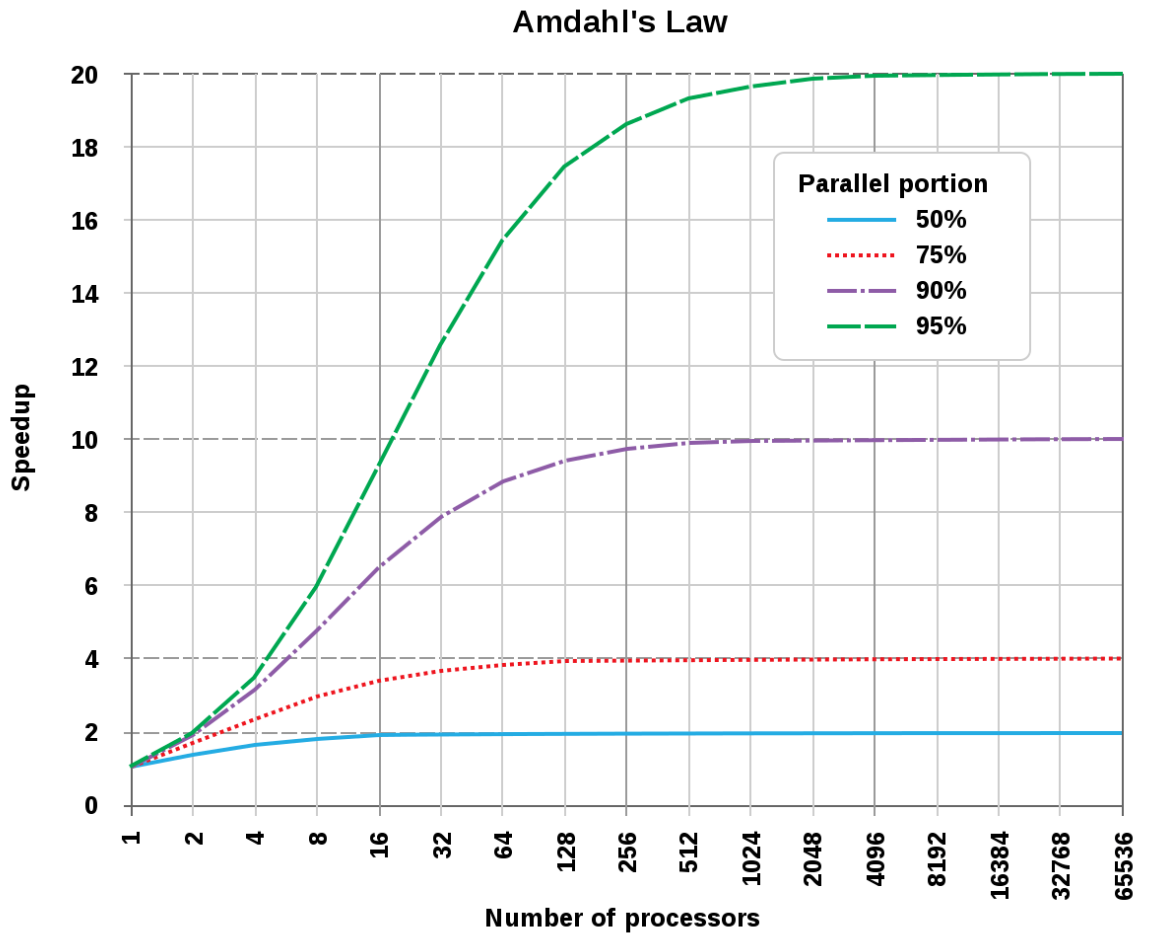
\includegraphics[width=0.65\linewidth]{img/amdahl'slaw.png}
    \caption{Amdahl’s Law}    
\end{figure}

\newpage
\section{Multi-thread models}

It could be dangerous to create a lot of threads, think about a virus that create lots of threads doing nothing only steel time CPU of others processes.

There are two different threads: 

\begin{itemize}
    \item[] \textbf{User thread} -- management done by user-level threads library (pthread, Windows thread, Java runnables and threads)
    \item[] \textbf{Kernel threads} -- Supported by the Kernel
\end{itemize}

\begin{figure}[htbp]
    \centering
    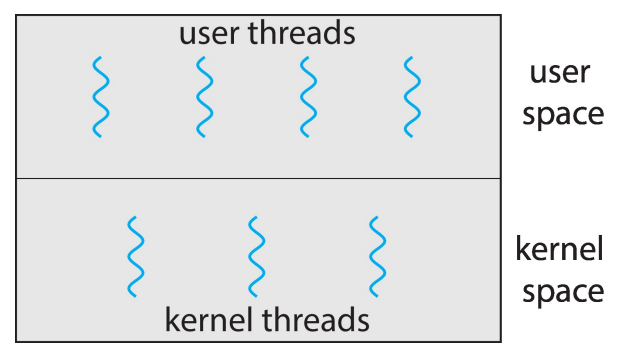
\includegraphics[width=0.5\linewidth]{img/user_space_thread.png}    
\end{figure}

The OS maps user and kernel thread in three way:

\begin{itemize}
    \item Many-to-One
    \item One-to-One
    \item Many-to-Many
\end{itemize}

\subsection{Many-to-One}

Many user-level threads mapped to single kernel thread, multiple threads may not run in parallel on multicore system because
only one may be in kernel at a time.

If one thread blocking causes all to block. This approach is use in a few OS like Solaris Green Threads or GNU Portable Threads.

\begin{figure}[htbp]
    \centering
    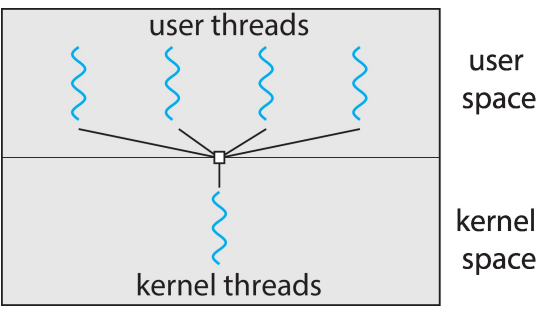
\includegraphics[width=0.5\linewidth]{img/MtM.png}
    \caption{Many-to-One thread}    
\end{figure}

\newpage
\subsection{One-to-One}

The easiest solution, each user-level thread maps to kernel thread this allows to more concurrency than many-to-one.

For the security the number of threads per process sometimes restricted due to overhead.

Some example are: \textbf{Windows} and \textbf{Linux} systems.

\begin{figure}[htbp]
    \centering
    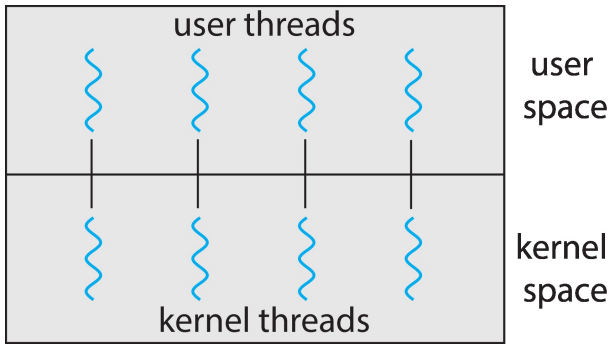
\includegraphics[width=0.5\linewidth]{img/OtO.png}
    \caption{One-to-One thread}    
\end{figure}

\subsection{Many-to-Many}
The last solution is a mix of the approach talked before.

Allows many user level threads to be mapped to many kernel threads if I have N user threads, I will be mapped into M ($\leq$ N) kernel threads this M size can be set by the OS, also considering the amount of
available cores, or the amount of processes allows the operating system to create a sufficient number of kernel
threads without over-creating them

Very complex to implement and manage.

Some example are: Windows with the ThreadFiber package, otherwise not very common.

\begin{figure}[htbp]
    \centering
    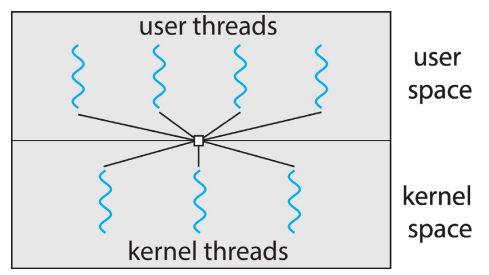
\includegraphics[width=0.5\linewidth]{img/MtMM.png}
    \caption{Many-to-Many thread}        
\end{figure}

\newpage
\subsection{Two-level Model: } similar to many-to-many, except that it allows a user thread to be bound to kernel thread. Not really used in practice.

\begin{figure}[htbp]
    \centering
    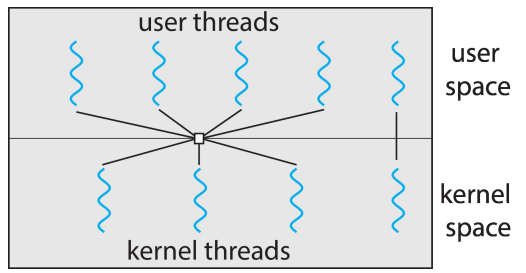
\includegraphics[width=0.5\linewidth]{img/TlT.png}
    \caption{Two-level Model}
    
\end{figure}

\newpage
\section{Thread libraries}
A Thread library provides programmer with API for creating and managing threads. Two primary ways of implementing: Library entirely in user space; Kernel-level library supported by the OS.

\subsubsection{Pthreads}
A POSIX standard (IEEE 1003.1c) API for thread creation and synchronization, is a Specification, not implementation. Infact API specifies behavior of the thread library, implementation is up to development of the library, this is common in UNIX OS (Linux and Mac OS X).
\paragraph{}
There are around 100 threads procedures, all prefixed pthread$\_$ and
they can be categorized into four groups:

\begin{itemize}
    \item Thread management – creating, joining threads etc.
    \item Mutexes
    \item Condition variables
    \item Synchronization between threads using read write locks and
barriers
    \item  Spinlocks
\end{itemize}


\subsubsection{Pthread\_attr\_init}

Initializes thread attributes, needed for creating new threads, by default it creates a structure like:

\begin{itemize}
    \item[] Detach state = PTHREAD\_CREATE\_JOINABLE 
    \item[] Scope = PTHREAD\_SCOPE\_SYSTEM
    \item[] Inherit scheduler = PTHREAD\_INHERIT\_SCHED
    \item[] Scheduling policy = SCHED\_OTHER
    \item[] Scheduling priority = 0
    \item[] Guard size = 4096 bytes
    \item[] Stack address = 0x40196000
    \item[] Stack size = 0x201000 bytes
\end{itemize}


\subsubsection{Pthread\_create}

Creates a new thread, initializing its tid, the function required some inputs:
\begin{itemize}
    \item The empty tid value (need to pass the address – by reference);
    \item The thread attributes (pass by reference, again);
    \item A pointer to the function to be exercised by the thread;
    \item Params of the function, as specified in the signature.
\end{itemize}

\begin{codeInC}
int pthread_create( pthread_t *restrict thread,
                    const pthread_attr_t *restrict attr,
                    void *(*start_routine)(void *),
                    void *restrict arg );
\end{codeInC}

In Linux when you call the create() function it means, create and run the thread.


\subsubsection{Pthread\_join}

The pthread\_join() function waits for the thread specified by thread to
terminate. If that thread has already terminated, then pthread\_join()
returns immediately. The thread specified by thread must be joinable.

Means that if a process calls the pthread\_join and the thread never
ends (stuck somewhere, …) the process will wait endlessly, it is called a \textbf{blocking function call}.

\begin{codeInC}
int pthread_join(pthread_t thread, void **retval);
\end{codeInC}

\subsubsection{Pthread\_exit}

The pthread\_exit() function terminates the calling thread and returns a
value via retval that (if the thread is joinable) is available to another
thread in the same process that calls pthread\_join().

To access the return value you have to provide a non-NULL pointer as
a second parameter of the pthread\_join function, this has to be typed as a void**.


\begin{codeInC}
[[noreturn]] void pthread_exit(void *retval);
\end{codeInC}

\paragraph{}
\textbf{Example: }


\begin{codeInC}

#include <pthread.h>
#include <stdio.h>

#include <stdlib.h>

int sum; /* this data is shared by the thread(s) */
void *runner (void *param); /* threads call this function */

int main(int argc, char *argv[]) {

    pthread_t tid; /* set the thread identifier */
    pthread_attr_t attr; /* set of thread attributes */
    
    /* set the default attributes of the thread */
    pthread_attr_init(&attr);
    /* create the thread */    
    pthread_create(&tid, &attr, runner, argv[1]);
    /* wait for the thread to exit */    
    pthread_join(tid, NULL);
    
    printf("sum = %d\n", sum);
}


/* The thread will execute in this function */
void *runner (void *param){

    int i, upper = atoi(param);
    sum = 0;
    
    for (i=1; i <= upper; i++)
        sum += i;
    
    pthread_exit(0);
}
\end{codeInC}


\subsection{JAVA THREADS}

When you write code in Java therads are managed by the JVM, typically implemented using threads model provided by underlying OS.

\paragraph{NOTE:} the JVM is a middlewere between your code and the host OS, thus uses OS-specific funztions.
\paragraph{}
Java thread may be created by:

\begin{itemize}
    \item Extending Thread class;
    \item Implementing the Runnable interface;
\end{itemize}

The standard practise to implement thread is to implement the \textbf{Runnable interface}:

\begin{codeInJava}
class Task implements Runnable{

    ...
    
    public void run(){
        System.out.println("I am a thread.");
    }

    ...
}

\end{codeInJava}

creation and waiting on a thread:

\begin{codeInJava}
import java.lang.Thread;

class Main {

    public static void main() {

        Thread worker = new Thread(new Task());
        worker.start();

        try{
            worker.join();
        }catch(InterruptedException ie){
            System.out.println("An error occurred.");
        }
        
    }
}
\end{codeInJava}

\newpage
\subsection{OpenMP}

In C, the process of creating a thread costs a lot of time and effort to the programmer. For this reason openMP libraries automatically implement the creation and the waiting.

Is a set of compiler directives and an API for C, C++, FORTRAN; it provides support for parallel
programming in shared-memory environments and identifies \textbf{parallel regions} – blocks of code that can run in
parallel. 
All of this only writing a single line: \verb|#pragma omp parallel|, it create as many threads as there are cores.

\begin{codeInC}
#include <omp.h>
#include <stdio.h>

int main(int argc, char *argv[]) {

    /* sequential code */
    
    #pragma omp parallel
    {                           //you must go to the new line
        printf("I am a parallel region.");
    }
    
    
    /* sequential code */
    
    return 0;
}
\end{codeInC}
\paragraph{}
There are different ways to make parallel code with omp, the code above defines a parallel region, which is code that will be executed by multiple threads in parallel, to enforce a given number of threads you should disable dynamic teams and specify the desired number of threads with either \verb|omp_set_num_threads()|:
\paragraph{}
\begin{codeInC}
#include <omp.h>

omp_set_dynamic(0);     // Explicitly disable dynamic teams
omp_set_num_threads(4); // Use 4 threads for all consecutive parallel regions

#pragma omp parallel ...
{
  // Code here will be run by 4 threads in parallel
}


\end{codeInC}
\paragraph{}
Or with the \verb|num_threads| OpenMP clause:
\paragraph{}
\begin{codeInC}
omp_set_dynamic(0);     // Explicitly disable dynamic teams
// Spawn 4 threads for this parallel region only

#pragma omp parallel... num_threads (4)
{
  // Code here will be run by 4 threads in parallel
}

\end{codeInC}

\newpage
\subsubsection{Directives}
There are different ways to make parallel code with omp.

\begin{itemize}
    \item \textbf{Pragma omp parallel } 
    \begin{itemize}
        \item[] Defines a parallel region, which is code that will be executed by multiple threads in parallel.
    \end{itemize}

    \item \textbf{Pragma omp for } 
    \begin{itemize}
        \item[] Causes the work done in a for loop inside a parallel region to be divided among threads.
    \end{itemize}

    \item \textbf{Pragma omp sections } 
    \begin{itemize}
        \item[] Identifies code sections to be divided among all threads.
        \item[] Each section has to be tagged as pragma omp section.
    \end{itemize}

    \item \textbf{Pragma omp single } 
    \begin{itemize}
        \item[] Lets you specify that a section of code should be executed on a single thread, not necessarily the main thread.
    \end{itemize}
\end{itemize}

If I only have one line of code within a parallel block, I just mark the single line with the last directives above.

\begin{codeInC}

int main(){

    ...

    #pragma omp parallel
    {

        //parallel

        #pragma omp single
        {
            // sequential
        }
        
        //parallel
    
    }

    return 0;
}
    
\end{codeInC}


\newpage
\section{Implicit threading}

Growing in popularity as numbers of threads increase, program correctness more difficult with explicit threads. Creation and management of threads done by compilers and run-time libraries rather than programmers (e.g. OpenMP).

This is called implicit threading, because the creation and all the waiting mechanisms of the thread are managed in the background.

\paragraph{Some methods to use implicit thread:}
\begin{itemize}
    \item Thread Pools
    \item Fork-Join
    \item OpenMP
    \item Grand Central Dispatch
    \item Intel Threading Building Blocks
\end{itemize}

\subsection{Thread Pools}

This library emulate OpenMP in Java language, it crate  a number of threads in a pool where they await work.

\paragraph{Some advantages:}

\begin{itemize}
    \item Usually slightly faster to service a request with an existing thread than create a new thread
    \item Allows the number of threads in the application(s) to be bound to the size of the pool
    \item Separating task to be performed from mechanics of creating task allows different strategies for running task
        \begin{itemize}
            \item[] E.g. Tasks could be scheduled to run periodically
        \end{itemize}
\end{itemize}

Three factory methods for creating thread pools in Executors class:

\begin{codeInJava}
static ExecutorService newSingleThreadExecutor();
static ExecutorService newFixedThreadPool(int size);
static ExecutorService newCachedThreadPool();
    
\end{codeInJava}


\paragraph{Example:}

\begin{codeInJava}
import java.util.concurrent.*;

public class ThreadPoolExample {

    public static void main(String[] args) {
    
        int numTasks = Integer.parseInt(args[0].trim());
        
        /* Create the thread pool */
        ExecutorService pool = Executors.newCachedThreadPool();
        
        /* Run each task using a thread in the pool */
        for (int i = 0; i < numTasks; i++)        
            pool.execute(new Task());
        
        /* Shut down the pool once all threads have completed */
        pool.shutdown();    
    }
}
    
\end{codeInJava}
\newpage

But also Windows API supports thread pools:

\begin{codeInJava}
DWORD WINAPI PoolFunction(AVOID Param){
    /*
    * This function runs as a separated thread.
    */
}
    
\end{codeInJava}


\subsection{Fork-Join Parallelism}

Multiple threads (tasks) are forked, and then joined, this allows to emulate parallelism (not threads) because it is a sub-process. Creation of sub-process is a heavy operation instead to create threads, also each fork have a copy of memory and not shared memory.

\begin{figure}[htbp]
    \centering
    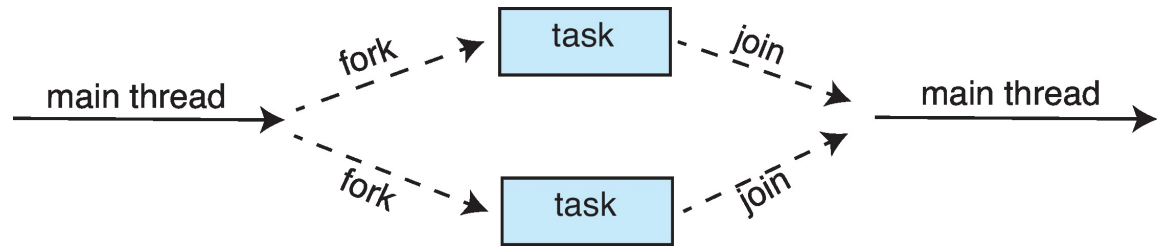
\includegraphics[width=0.7\linewidth]{img/fork_join.png}
\end{figure}

\paragraph{General algorithm for fork-join strategy:}

\begin{codeInC}
Task(problem)   

if problem is small enough 
    then 
        solve the problem directly 
else
    then
        subtask1 = fork(new Task(subset of problem))                
        subtask2 = fork(new Task(subset of problem))                
        result1 = join(subtask1)                                        
        result2 = join(subtask2)   
endif

return combined results                                    

\end{codeInC}

\begin{figure}[htbp]
    \centering
    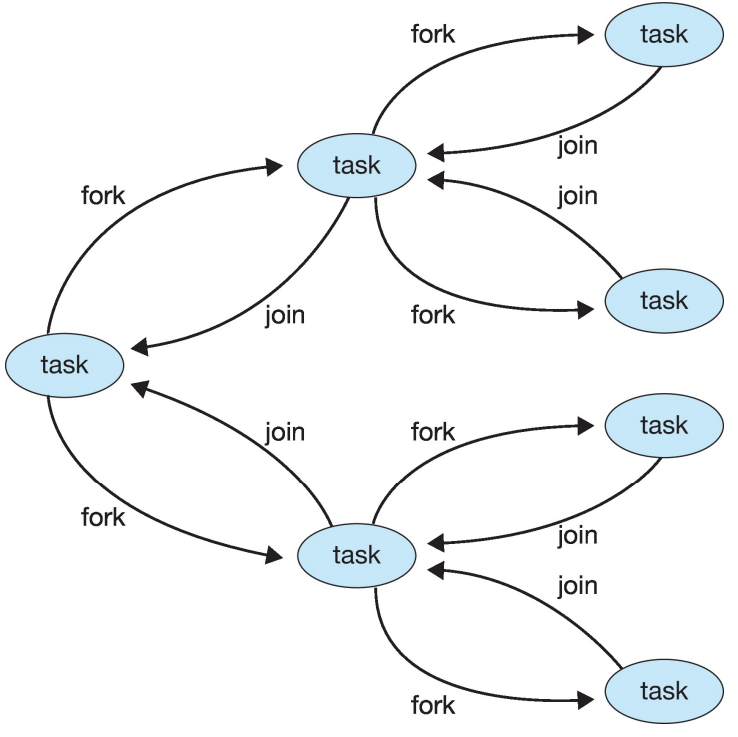
\includegraphics[width=0.5\linewidth]{img/F_J_parall.png}
    \caption{Fork-Join Parallelism state machine}    
\end{figure}







\newpage
\section{CPU scheduling}

So far we have talked about processes and threads: what they are, how to implement them, how to increase maximum speed, how to use libraries to implement them, etc.

Now we want to know the behavior of all this, how the operating system interacts and handles these activities.


\subsection{Basic Concepts}

We want to maximize CPU utilization obtained with multiprogramming. The tasks are only CPU burst and I/O burst: Process
execution consists of a cycle of CPU execution and I/O wait, in the same order.

The CPU burst distribution is of main concern.

\begin{figure}[htbp]
    \centering
    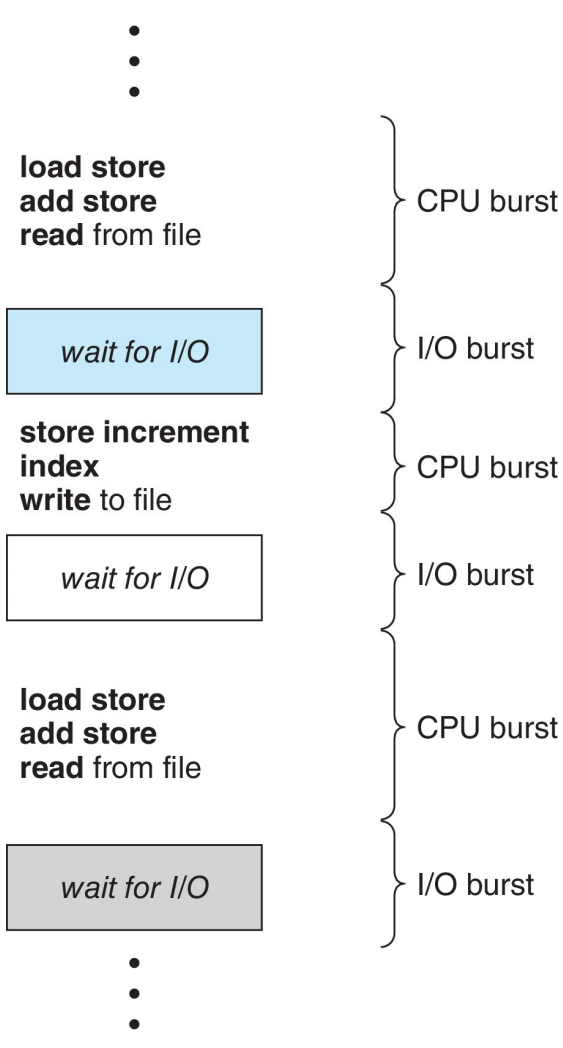
\includegraphics[width=0.35\linewidth]{img/CPU_BURST.png}
    
    
\end{figure}

So, if a programme  that performs sorting uses the CPU, but when it waits for some I/O the tasks does not use CPU and we want to pull it out from the CPU because others process want use it.


\paragraph{Histogram of CPU-burst Times}
Large number of short bursts and small number of longer bursts.
\begin{figure}[htbp]
    \centering
    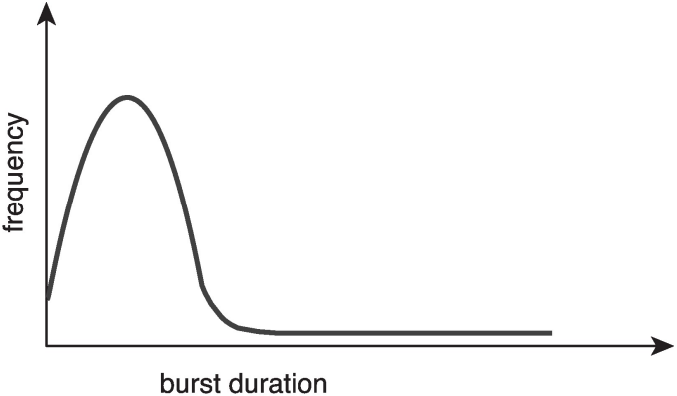
\includegraphics[width=0.4\linewidth]{img/vurst.png}
    
    
\end{figure}

\newpage
\subsection{CPU Scheduler}
The CPU Scheduler working to dispatching tasks to all the cores of the CPU. 

The CPU scheduler selects from among the processes in ready queue, and allocates a CPU core to one of them: Queue may be ordered in various ways.

\paragraph{}
So far, in fact when a task enters the CPU we do not have a method to kick it out and take another one from the ready queue an put it into the cpu, we waiting until it ends.

For this reasons CPU scheduling decisions may take place when a process:
\begin{enumerate}
    \item Switches from running to waiting state
    \item Switches from running to ready state
    \item Switches from waiting to ready
    \item Terminates
\end{enumerate}

For situations 1 and 4, there is no choice in terms of managing the
ready queue. Simply, a new process is taken from the queue.

For situations 2 and 3, however, there is a choice that is up to the
scheduler.

\begin{figure}[htbp]
    \centering
    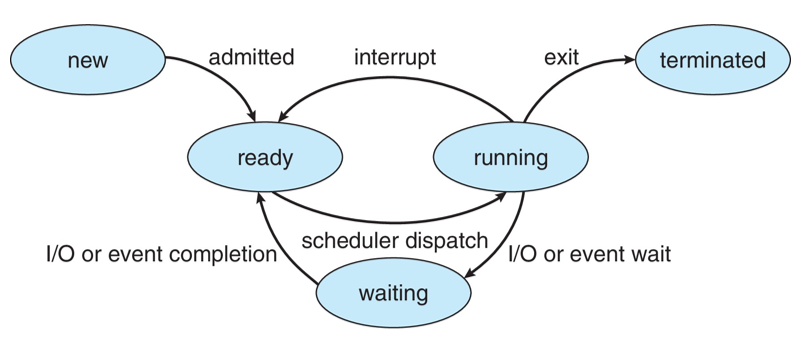
\includegraphics[width=0.65\linewidth]{img/process_state_diagram.png}
    \caption{Diagram of Process State}    
\end{figure}

\subsection{Preemptive and Nonpreemptive Scheduling}

Under \textbf{Nonpreemptive scheduling}, once the CPU has been
allocated to a process, the process keeps the CPU until it
releases it either by \textbf{terminating} or by switching to the \textbf{waiting
state}.

Otherwise, it is \textbf{preemptive}.

Thus, a process could theoretically keep it forever, or, before the OS recognizes this anomalous behavior
and kills it.

\paragraph{}
Virtually all modern operating systems including Windows, MacOS, Linux, and UNIX use preemptive scheduling algorithms.
This methods allows to set a priority to each tasks.

\subsubsection{Preemptive Scheduling and Race Conditions}

Preemptive scheduling can result in race conditions when data are
shared among several processes.

\paragraph{}

Consider the case of two processes that share data. While one
process is updating the data, it is preempted so that the second
process can run. The second process then tries to read the data,
which are in an inconsistent state (data consistency).

\begin{codeInC}
void myFunction(){
    int myID = thread;
    myID++;
}

\end{codeInC}

If it is nonpreemptive the function stuck into the cpu untill the function \verb|myFunction()| terminate (line: 5), otherwise if it is preemptive the CPU scheduler may stopped the execution at line 3 another process could execute the function and the two process have the same myID.

\paragraph{Note:} these problems happen only when one process writes and at
least another one tries to read it.
Read-only variables or atomic block will never have any kind of problems and can
be shared without issues.

\subsection{Dispatcher}
Assume that the CPU decided that a given task P1 has to be assigned to a core now running P0. Then what?

Dispatcher module gives control of the
CPU to the process selected by the CPU
scheduler; this involves:

\begin{itemize}
    \item Switching context;
    \item Switching to user mode;
    \item Jumping to the proper location in the user program to restart that program;
\end{itemize}

\begin{figure}[htbp]
    \centering
    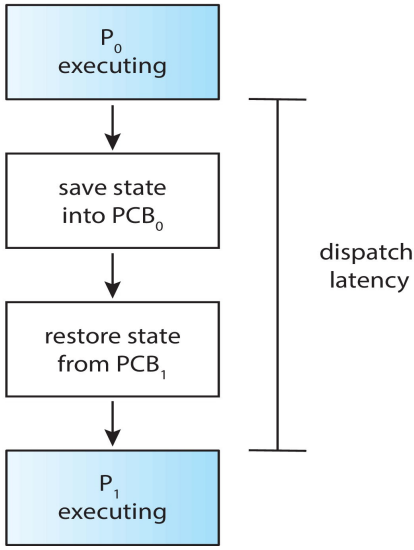
\includegraphics[width=0.3\linewidth]{img/dispacher.png}
    \caption{Dispatcher}    
\end{figure}

\textbf{Dispatch latency} – time it takes for the dispatcher to stop one process and start another running. The preemptive don't give nothing for free.

\subsection{Scheduling Criteria}

There are some parameters that the CPU scheduler could optimize, but not all of them because some of some of them conflict.

\begin{itemize}
    \item \textbf{CPU utilization} - keep the CPU as busy as possible;
    \item \textbf{Throughput} – \# of processes that complete their execution per time unit;
    \item \textbf{Turnaround time} – amount of time to execute a particular process;
    \item \textbf{Waiting time} – the amount of time a process has been waiting in the ready queue;
    \item \textbf{Response time} – amount of time it takes from when a process enters the ready queue to when it gets into the CPU the first time. 
\end{itemize}

The first two are connected. 

\newpage
\section{Scheduling Algorithms}

\subsection{FCFS}

\begin{figure}[htbp]
    \centering
    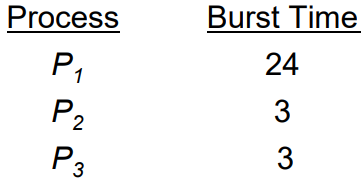
\includegraphics[width=0.25\linewidth]{img/FCFS.png}
    \caption{First- Come, First-Served}    
\end{figure}

The First-Come, First-Served Scheduling is non preemptive: once assigned, a process finishes is
execution.

\paragraph{}

\textbf{Waiting time} for P1, P2, P3: 0, 24, 27;
\textbf{Average waiting time}: $(0 + 24 + 27)/3 = 17$.

\paragraph{}
But if the processes arrive in the order: P2,P3,P1, we obtain other number:

\textbf{Waiting time} for P1, P2, P3: 6, 0, 3;
\textbf{Average waiting time}: $(6 + 0 + 3)/3 = 3$.

Much better than previous case. This case is called \textbf{convoy effect} - short process behind long process.

\subsection{SJF}
Shortest-Job-First Scheduling or, better, shortest-next-CPU-burst. This method minimize the waiting time.

\paragraph{}
Associate with each process the length of its next CPU burst, but there is a big problem: How do we determine the length of the next CPU burst?

\begin{itemize}
    \item Could ask the user:  unfeasible, introduces delays;
    \item Estimate but how?
\end{itemize}


\subsubsection{Determining Length of Next CPU Burst}
Can be done by using the length of previous CPU bursts (of the same task), using exponential averaging:

\begin{equation}
    \tau_{n+1} = \alpha t_n + (1+\alpha)\tau_n
\end{equation}

where:
\begin{itemize}
    \item $t_n$: actual length of the $n^{th}$ CPU burst;
    \item $\tau_{n+1}$: predicted value for the next CPU burst
    \item $\alpha$ set to 0.5, $ 0 \leq \alpha \leq 1$ 
\end{itemize}

\newpage

\begin{figure}[htbp]
    \centering
    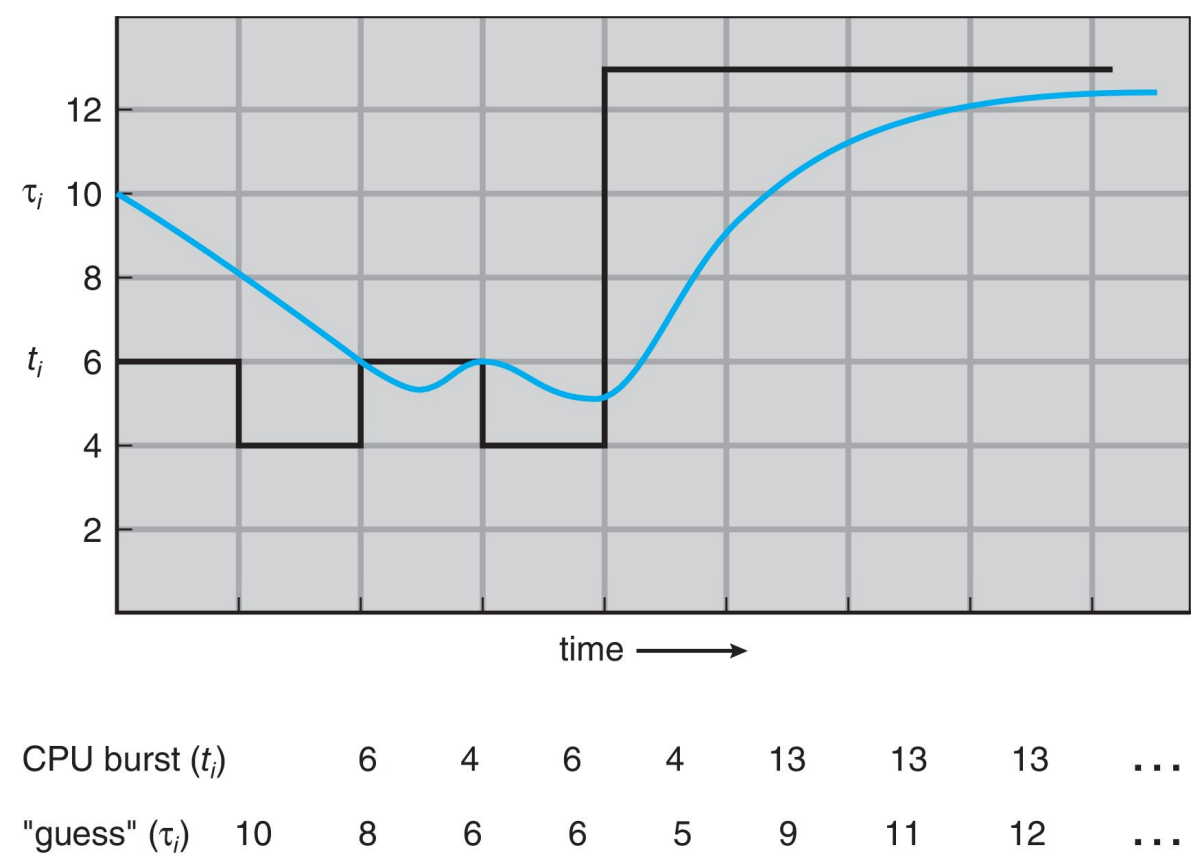
\includegraphics[width=0.55\linewidth]{img/prediction.png}
    \caption{Prediction vs Actual CPU Burst}    
\end{figure}


This method is precise if the CPU burst does not change a lot.

\subsection{SRT}

The Shortest-Remaining-Time-first is the preemptive version of SJN. Whenever a new process arrives in the ready queue, the
decision on which process to schedule next is redone using the SJN algorithm.

Is SRT more “optimal” than SJN in terms of the minimum average waiting time for a given set of processes?


\begin{figure}[htbp]
    \centering
    \includegraphics[width=0.65\linewidth]{img/SRTF.png}
  
\end{figure}

\newpage
\subsection{Round Robin}

Each process gets a small unit of CPU time (\textbf{time quantum} or \textbf{time slice} q), usually 10-100 milliseconds. After this time has elapsed, the process is preempted and added to the end of the ready queue.

If there are n processes in the ready queue and the time quantum
is q, then each process gets 1/n of the CPU time in chunks of at
most q time units at once. No process waits more than \textbf{(n-1)q}
time units.

\paragraph{}
Timer interrupts every quantum to schedule next process.

\paragraph{Performance:}
\begin{itemize}
    \item [] q large: FIFO (FCFS);
    \item [] q small: RR.
\end{itemize}

\paragraph{NOTE:} the q must be larger with respect to context switch, otherwise overhead is to high, there will be no execution, just context switches after context switches (useless).


\subsubsection{RR vs FCFS}


\begin{figure}[htbp]
    \centering
    \includegraphics[width=0.6\linewidth]{img/RR.png}    
    
\end{figure}

Typically, higher average turnaround than SJF, but better \textbf{response}:
\begin{itemize}
    \item[] Waiting Average = (6 + 4 + 7) / 3 = 5.7
    \item[] Turnaround = (30 + 3 + 3) / 3 = 12
    \item[] Response = (4 + 7 + 10) / 3 = 7 
\end{itemize}

\begin{figure}[htbp]
    \centering
    \includegraphics[width=0.6\linewidth]{img/FSCS_VSR.png}   
    
\end{figure}

\begin{itemize}
    \item[] Waiting Average =  (0 + 24 + 27) / 3 = 17
    \item[] Turnaround =  (24 + 3 + 3) / 3 = 10
    \item[] Response = (0 + 24 + 27) / 3 = 17 
\end{itemize}

\subsubsection{Turnaround Time Varies With The Time Quantum}

Rule of Thumb: 80\% of CPU bursts should be shorter than q.

\paragraph{Example: } processes P1, P2, P3, P4 with respectively time 6, 3, 1, 7; a good q could be 6.

\newpage
\section{Priority Scheduling}

A priority number (integer) is associated with each process. The CPU  is allocated to the process with the highest priority, smaller integer $\equiv$ highest priority.

\begin{itemize}
    \item Preemptive: the scheduler kick the task out the CPU for some reasons;
    \item Non-preemptive: the scheduler must not kick the task out the CPU unless it waiting for an I/O.
\end{itemize}

But not all the tasks are the same, in fact there are users threads and kernel threads. This latter should not be blocked by the users threads.

\paragraph{}
\textbf{SJV} is a priority scheduling where priority is the inverse of the predicted next CPU bust. Regardless to all the algorithm chose the tasks that have the higher priority, it means it have the lower CPU burst time.


But there is a problem:

\begin{itemize}
    \item[] \textbf{Starvation} - low priority tasks may never execute
\end{itemize}

The solution of this problem is called:

\begin{itemize}
    \item[] \textbf{Aging} - if tasks does not execute in n-time, its priority (age) is increased, this process is repeated until the execution arrives. The more a process remains in the ready queue, the more his priority (age) increase.
\end{itemize}

e.g. if the tasks is in the ready queue for 4 CPU burst, I increase its priority.

\subsubsection{Example of Priority Scheduling}

\begin{figure}[htbp]
    \centering
    \includegraphics[width=0.4\linewidth]{img/priority_sched.png}  
\end{figure}

The scheduler in this situation does not take care about the CPU burst time, it look at the priority of the process.

\begin{figure}[htbp]
    \centering
    \includegraphics[width=0.65\linewidth]{img/gantt.png}
\end{figure}

This priority scheduling has an average waiting time of 8.2. But the burst of CPU of course is important for improving average waiting.
\paragraph{}

But if the processes are the same priority? There is some mechanism that allow to chose one or the other tasks, we can chose different type of scheduling algorithms:

\begin{itemize}
    \item Priority scheduling with Round-Robin - same priority, the tasks to execute first is chose by the random algorithm;
    \item Priority scheduling with FCFS - same priority, the tasks to execute first is chose by the first come first served algorithm;
    \item Priority scheduling with SJF - same priority, the tasks to execute first is chose by shortest jobs first algorithm;
    \item Other.
\end{itemize}

\begin{figure}[htbp]
    \centering
    \includegraphics[width=0.5\linewidth]{img/PSWRR.png}
    \caption{Priority Scheduling w/ Round-Robin}    
\end{figure}

\section{Scheduling in using multiple queues}

Having different priority queues for all the priority level in the OS, allow to implement different scheduling algorithms for each queues to decide witch tasks going to be execute first.

\subsection{Multilevel queue}
Multilevel queue scheduler defined by the following parameters:

\begin{itemize}
    \item Number of queues;
    \item Scheduling algorithms for each queue;
    \item Method used to determine which queue a process will enter;
    \item when that process needs service;
    \item Scheduling among the queues.
\end{itemize}


With priority scheduling, have separate queues for each priority.

\begin{figure}[htbp]
    \centering
    \includegraphics[width=0.35\linewidth]{img/multileve_queue.png}
    \caption{Multilevel queue}    
\end{figure}

Aging can be implemented using multilevel feedback queue.

\paragraph{Example of multilevel feedback queue: } we look at the CPU bust and not to the priority.

\paragraph{}
Three queues:
\begin{itemize}
    \item Q0 – RR with time quantum 8 milliseconds
    \item Q1 – RR time quantum 16 milliseconds
    \item Q2 – FCFS
\end{itemize}

\newpage
Scheduling:  A new process enters queue Q0 which is served in RR

\begin{itemize}
    \item[--] When it gains CPU, the process receives 8 milliseconds
    \item[--] If it does not finish in 8 milliseconds, the process is moved to queue Q1
\end{itemize}

At Q1 job is again served in RR and receives 16 additional milliseconds, if it still does not complete, it is preempted and moved to queue Q2.

\begin{figure}[htbp]
    \centering
    \includegraphics[width=0.45\linewidth]{img/multilever_queue.png}
\end{figure}

\subsection{Scheduling in multiprocessor systems}

CPU scheduling more complex when multiple CPUs are available, in fact multiprocess may be any one of the following architectures:

\begin{itemize}
    \item Multicore CPUs
    \item Multithreaded cores - the OS think to have double core 
    \item Heterogeneous multiprocessing
\end{itemize}

When you buy new processor on the box is written: this processor have L1, L2 and L3 cache. It means that the L1 cache is the private cache of the single core, this is divide in 2, L2 is the cache shared by the core, and the L3 cache is the cache shared by all core.

\subsubsection{Symmetric multiprocessing}
Symmetric multiprocessing (SMP) is where each processor is self scheduling.

\begin{itemize}
    \item All threads may be in a common ready queue (a) - more easier to implement, all tasks occupy the uncommitted core
    \item Each processor may have its own private queue of threads (b) - faster in context-switching, virus attack only one core
\end{itemize}


\begin{figure}[htbp]
    \centering
    \includegraphics[width=0.55\linewidth]{img/SMP.png}   
    
\end{figure}


\subsection{Multi-core Processors}
Recent trend to place multiple cores on same physical chip, this approach is faster and consumes less power.

Multiple threads per core (virtual cores) also growing:

\begin{itemize}
    \item Takes advantage of memory stall to make progress on another thread while memory retrieve happens
    \item Each core has > 1 hardware threads
    \item If one thread has a memory stall, switch to another thread!
\end{itemize}

for those reason the L1 is divide in 2 or more area, witch each contains the data to another thread.

\begin{figure}[htbp]
    \centering
    \includegraphics[width=0.6\linewidth]{img/memory_stall.png}   
    
\end{figure}

Chip-multithreading (CMT)
assigns each core multiple
hardware threads. (Intel refers
to this as hyperthreading.)

E.g. On a quad-core system with 2
hardware threads per core, the
operating system sees 8 logical
processors or virtual core.


\begin{figure}[htbp]
    \centering
    \includegraphics[width=0.35\linewidth]{img/hyperthreading.png}
    \caption{Chip-multithreading}    
\end{figure}

Also there are two level of scheduling:

\begin{enumerate}
    \item The operating system deciding which software thread to run on a logical CPU
    \item Each core decides which hardware thread to run on the physical core.
\end{enumerate}

\begin{figure}[htbp]
    \centering
    \includegraphics[width=0.5\linewidth]{img/level_thread.png}    
    
\end{figure}

\newpage
\subsubsection{Processor Affinity}
When a thread has been running on one processor, the cache contains some information and data and if the process return into the CPU it take the previous data from cache, this benefit in term of latency. We refer to this as a thread having affinity for a processor (i.e.
“processor affinity”).


\paragraph{}
Load balancing may affect processor affinity as a thread may be moved
from one processor to another to balance loads, yet that thread loses
the contents of what it had in the cache of the processor it was moved
off of.


\begin{itemize}
    \item \textbf{Soft affinity} – the operating system attempts to keep a thread running on the same processor, but no guarantees
    \item \textbf{Hard affinity }– allows a process to specify a set of processors it may run on.
\end{itemize}

\newpage
\section{Real time CPU scheduling}

For some reason, the tasks required to be execute in a specific time, or in real-time, e.g. ABS, train tracking and so on. They can present obvious challenges, there are two way to implement this functionality:

\begin{itemize}
    \item \textbf{Soft real-time systems} – Critical real-time tasks have the highest priority, but no guarantee as to when tasks will be scheduled;
    \item \textbf{Hard real-time systems} – task must be serviced by its deadline
\end{itemize}

\subsection{Latencies}
\textbf{Event latency} – the amount of time that elapses from when an event occurs to when it is serviced. There are two tipes of latencies affect performance: 

\textbf{Interrupt latency} – time from arrival of interrupt to start of routine that services interrupt
\textbf{Dispatch latency }– time for schedule to take current process off CPU and switch to another


\begin{figure}[htbp]
    \centering
    \includegraphics[width=0.45\linewidth]{img/latency.png}
    
    
\end{figure}


\subsection{Priority-based Scheduling}

For real-time scheduling, scheduler must support preemptive, prioritybased scheduling. But only guarantees \textbf{soft real-time}.

For hard real-time must also provide ability to meet \textbf{deadlines}.
\paragraph{}
Processes have new characteristics: \textbf{periodic} ones require CPU at constant intervals; this process has:

\begin{itemize}
    \item processing time t;
    \item deadline d;
    \item period p.
\end{itemize}

Rate of periodic task is 1/p


\begin{figure}[htbp]
    \centering
    \includegraphics[width=0.75\linewidth]{img/priority_base.png}   
    
\end{figure}

\subsubsection{Rate Monotonic Scheduling (RMS)}
The priority is assigned based on the inverse of its period, priority = 1/period.

\begin{itemize}
    \item[] Shorter periods = higher priority;
    \item[] Longer periods = lower priority.
\end{itemize}

\paragraph{Example: } P1 is assigned a higher priority than P2, P1 has deadline 50, P2 has deadline 100

\begin{figure}[htbp]
    \centering
    \includegraphics[width=0.7\linewidth]{img/RMP.png}
    
\end{figure}

RMS in not optimal solution, P1 is far from its deadline, but P2 is less far from its deadline. 

\subsubsection{Earliest Deadline First Scheduling (EDF)}

In this case the priorities are assigned according to deadlines:

\begin{itemize}
    \item[] The earlier the deadline, the higher the priority
    \item[] The later the deadline, the lower the priority
\end{itemize}


\begin{figure}[htbp]
    \centering
    \includegraphics[width=0.7\linewidth]{img/EDF.png}
    
    
\end{figure}

All of this type of scheduling algorithms must have the minimum requirements of core numbers.

\newpage
\section{OS scheduling examples}

\subsection{Linux Scheduling in Version 2.6.23+}

The Linux scheduling is based on Completely Fair Scheduler (CFS). It is composed of:

\paragraph{Scheduling classes: } each tasks has specific priority, scheduler picks highest priority task in highest scheduling class, rather than quantum based on fixed time allotments, based on proportion of CPU time.

Two scheduling classes included, others can be added:

\begin{enumerate}
    \item default;
    \item real-time.
\end{enumerate}

\paragraph{Virtual run time:} CFS scheduler maintains per task virtual run time in variable \verb|vruntime|. Associated with decay factor based on priority of task – lower priority
is higher decay rate, normal default priority yields virtual run time = actual run time.

\paragraph{}
To decide next task to run, scheduler picks task with lowest virtual run time. But how to implement all of this?

\paragraph{}
To decide witch tasks to run the CFS looks at the \verb|vruntime|, the smartest way to implement this is to see the ready queue like a btree. In this way you have the smallest value always in the same position.


\begin{figure}[htbp]
    \centering
    \includegraphics[width=0.5\linewidth]{img/btree.png}
    
    
\end{figure}


\subsection{Windows Scheduling}

Windows uses priority-based preemptive scheduling. Highest-priority thread runs next.
\textbf{Dispatcher} is scheduler.  

Windows has a 32-level priority scheme, where \textbf{Variable class} is 1-15, \textbf{real-time class} is 16-31. Priority 0 is memory-management thread.

It is a multilevel queue for each level and if no run-able thread, it runs \textbf{idle thread} a task that do noting.


\begin{figure}[htbp]
    \centering
    \includegraphics[width=0.7\linewidth]{img/WP.png}
    \caption{Windows priorities}
    
\end{figure}


\subsection{Solaris}

The Solaris OS is used for business. This OS is Priority-based scheduling and has six classes of priority available:


\begin{itemize}
    \item Time sharing (default) (TS)
    \item Interactive (IA)
    \item Real time (RT)
    \item System (SYS)
    \item Fair Share (FSS)
    \item Fixed priority (FP)
\end{itemize}

Given thread can be in one class at a time and  each class has its own scheduling algorithm. Time sharing is multi-level feedback queue, loadable table configurable by sysadmin.

\begin{figure}[htbp]
    \centering
    \includegraphics[width=0.4\linewidth]{img/ssolaris.png}
    \caption{Solaris scheduling}
    
\end{figure}

\newpage
\section{Scheduling evaluation}

The scheduling algorithm depends on who is the final users: reading mail, surfing on internet, coding, gaming, render a video, etc. all this tasks required different CPU burst and  we would implement a  \textbf{Deterministic model} to know the CPU burst.

The analytic evaluation is used to takes a particular predetermined workload and defines the performance of each algorithm for that workload.

\subsubsection{Consider 5 processes arriving at time 0:}


\begin{table}[htbp]
    \centering
    \begin{tabular}{cc}
        Processes & Burst Time\\
        \hline
        P1 & 10 \\
        P2 & 29\\
        P3 & 3\\
        P4 & 7\\
        P5 & 12\\
    \end{tabular}
\end{table}

The Deterministic Evaluation for each algorithm, calculate minimum average waiting time, simple and fast, but requires exact numbers for input, applies only to those inputs:

\begin{itemize}
    \item FCS is $28ms$
    \item Non-preemptive SFJ is $13ms$
    \item RR is $23ms$
\end{itemize}


 This deterministic model is not applicable in the real-word.

 \subsection{Queueing models}
Queueing models are mathematical tools used to analyze systems where customers (or items) wait for service. This model describes the arrival of processes, and CPU and I/O bursts probabilistically. These models help predict things like average queue lengths, waiting times, server utilization, and the probability of having a certain number of customers in the system.

Computer system described as network of servers, each with queue of waiting processes

\subsubsection{Little's Formula}

Little’s law – in steady state, processes leaving queue must
equal processes arriving, thus:

\begin{equation*}
    n = \lambda W
\end{equation*}

Where:

\begin{itemize}
    \item[] n = average queue length
    \item[] W = average waiting time in queue
    \item[] $\lambda$ = average arrival rate into queue
\end{itemize}

For example, if on average 7 processes arrive per second, and
normally 14 processes in queue, then average wait time per
process = 2 seconds; but if I have a CPU that can execute only 6 tasks per second the queue grow.


\newpage
\paragraph{Problem: }very rough estimate.

\subsection{Simulations}

Queueing models limited, \textbf{Simulations} more accurate. Is a virtual model, more the model is close to the real behavior and more the simulation is real and the statistics accurate.

Other option is just implement new scheduler and test in the real system, this involves:

\begin{itemize}
    \item High cost, high risk
    \item Environments vary
\end{itemize}

The simulation is one of the possible low cost solution to try new scheduler.


\chapter{Synchronization Tools}


\section{Critical section and race condition}
For now we know: to create tasks, the tasks have a own life, scheduling algorithms. But how we manage it?

\paragraph{Problem:} in a dual core processor each process has own life, if in the same time two process call the fork() call, the sub-processes have the same PID! This may happen because in the dual-core processor the tasks are execute in parallel. 

\paragraph{}
This problem also happen even if we have a single-core CPU, because if the OS has the preemption mechanism in each time the function fork() can be kicked out of the CPU before increase the PID number, the another tasks call the same function and after that we have the same problem saw before: two tasks with same PID.

\paragraph{}
This is called \textbf{race condition}, and implies the inconsistency of the data read. We want to maintaining this consistency of data.

\paragraph{NOTA:} the race condition and the inconsistency of the data happen \textbf{only} if the variable is in the read/write mode, this not happen if the variable is only in read mode!


\begin{figure}[htbp]
    \centering
    \includegraphics[width=0.65\linewidth]{img/race_cond.png}
    \caption{Race condition on kernel variable next\_available\_pid}    
\end{figure}


\newpage
\subsection{Critical section}
Consider system of n processes, each process has critical section segment of code: process may be changin common variables, updating tables, etc.

When one process in critical section, no other may be in its critical section, \textbf{Critical section problem} is to design protocol to solve this.

Each process must:

\begin{itemize}
    \item ask permission to enter critical section in entry section,
    \item may follow critical section with exit section,
    \item then remainder section
\end{itemize}

\begin{codeInC}
while( true ){
    ...
    
    //entry into critical section
        critical section
    //exit critical section
    
    ...
}
\end{codeInC}


\subsection{Critical section problem}
Requirements for solution to critical-section problem:

\begin{itemize}
    \item \textbf{Mutual Exclusion} - If process Pi is executing in its critical section, then no other processes can be executing in their critical sections; no more one in the same critical section;
    \item \textbf{Progress} - If no process is executing in its critical section and there exist some processes that wish to enter their critical section, then the selection of the process that will enter the critical section next cannot be postponed indefinitely; if no one tasks are into the critical section other process may access into it;
    \item \textbf{Bounded Waiting} - A bound must exist on the number of times that other processes are allowed to enter their critical sections after a process has made a request to enter its critical section and before that request is granted; if a tasks want to enter into the critical section must waiting to have the access.
\end{itemize}

If your system has a \textbf{single core} CPU and is \textbf{nonpreemtive} OS, you never have this problem, but the question is: who in 2024 does not have a multi-core CPU inside a PC? None.
\newpage
\section{Software solutions 1}
Assume that the \textbf{load} and \textbf{store} machine-language instructions are atomic; that is, cannot be interrupted. 

Two processes share one variable called: int turn, this variable indicates who can access the critical section. Initially, the value of turn is set to i.

\begin{codeInC}
while (true){
    while (turn = = i);
    /* critical section */
    turn = i;
    /* remainder section */
}
\end{codeInC}


\begin{codeInC}
while (true){
    while (turn = = j);
    /* critical section */
    turn = j;
    /* remainder section */
}
\end{codeInC}

\paragraph{Correctness of this Software Solution:} 

\begin{itemize}
    \item \textbf{Mutual exclusion} is preserved, since Pi enters critical section only if turn == i;
    \item \textbf{Progress requirements} is not respected. The other task can not access into its critical section;
    \item \textbf{Bounded-waiting}, also, is not respected. Process J may be waiting for the critical section endlessly.
\end{itemize}


\subsection{Peterson’s Solution}

Same as before: two process, load and store machine-language instructions are atomic.

The change is: two processes share two variables: int turn and boolean flag[2]. The first indicates which processes enters the critical section, and the flag array is used to indicate if a process is ready to enter the critical section, flag[i] = true -> the process Pi is ready.

\paragraph{Peterson’s Algorithm for Process Pi}


\begin{codeInC}
while (true){
    flag[i] = true;
    turn = j;
    while (flag[j] && turn = = j);
    
    /* critical section */
    
    flag[i] = false;
    
    /* remainder section */
}
\end{codeInC}

\newpage
\paragraph{Correctness of Peterson’s Solution:} 

\begin{itemize}
    \item \textbf{Mutual exclusion} is preserved, since Pi enters critical section only if turn == i, either flag[j] = false or turn = i;
    \item \textbf{Progress requirements} is satisfied.
    \item \textbf{Bounded-waiting}, requirement is met. If it is the turn of the other, but the other is not willing to enter the critical
section, the first process will enter (even if not its turn technically).
\end{itemize}

Although useful for demonstrating an algorithm, Peterson’s
Solution is not guaranteed to work on modern architectures. To improve performance, processors and/or compilers may
reorder operations that have no dependencies.

For single-threaded this is ok as the result will always be the
same. 
For multithreaded the reordering may produce inconsistent or
unexpected results! Ideally, you want a single instruction for entry/exit section.

\subsection{Reordering}

The compiler transform the high programme language into binary code, but for optimization it happen that some operation are physically distant, and the preemption could cause some error.

\subsection{Peterson vs Multi-Threading}
The effects of instruction reordering in Peterson’s Solution

\begin{figure}[htbp]
    \centering
    \includegraphics[width=0.65\linewidth]{peterson.png}    
    
\end{figure}

This allows both processes to be in their critical section at the same
time, to ensure that Peterson’s solution will work correctly on modern
computer architecture we must use a \textbf{Memory Barrier}.
\newpage
\section{Memory Barrier}

Memory models may be either:

\begin{itemize}
    \item \textbf{Strongly ordered} – where a memory modification of one processor is immediately visible to all other processors.
    \item \textbf{Weakly ordered} – where a memory modification of one processor may not be immediately visible to all other processors
\end{itemize}

A memory barrier is an instruction that forces any change in memory to be propagated (made visible) to all other processors.

\paragraph{}
I need some barrier line that tells to compiler that it can reorder instruction before and after the barrier. In this way the consisntency of the data are ok.

\paragraph{Example:} boolean flag = false; int x = 0;
\begin{codeInC}
//thread one
while (!flag)

memory_barrier();
print x;
\end{codeInC}
\begin{codeInC}
//thread two
while (!flag)

memory_barrier();
print x;
\end{codeInC}

For Thread 1 we are guaranteed that that the value of flag
is loaded before the value of x.

For Thread 2 we ensure that the assignment to x occurs
before the assignment flag.

\paragraph{}
If we do not write \verb|memory_barrier();| the programm print the value of 0, before the value x is set bt thread 2.

\newpage
\section{Hardware instructions}

How to implement all of this in the language programm?

\paragraph{}
Many systems provide hardware support for implementing the critical section code.
We will look at three forms of hardware support:
\begin{itemize}
    \item Hardware instructions
    \item Atomic variables
\end{itemize}

\subsection{Hardware Instructions}
Special hardware instructions that allow us to either
test-and-modify the content of a word, or to swap the
contents of two words atomically: 

\begin{itemize}
    \item[] Test-and-Set instruction
    \item[] Compare-and-Swap instruction
\end{itemize}


\subsubsection{test\_and\_set instruction}

\begin{codeInC}
boolean test_and_set (boolean *target){
    boolean rv = *target;
    *target = true;
    return rv:
}
\end{codeInC}

Properties:

\begin{itemize}
    \item Executed atomically
    \item Returns the original value of passed parameter
    \item Set the new value of passed parameter to true
    \item No changes if target is already true
\end{itemize}

Shared boolean variable lock, initialized to false:

\begin{codeInC}
do {
    while (test_and_set(&lock)); /* do nothing */
    /* critical section */
    lock = false;
    /* remainder section */
} while (true);

\end{codeInC}

After the first process, any process can go in. There is no
queue maintained, so any new process that finds the lock to
be false again can enter. So bounded waiting is not
ensured.

\paragraph{}
The \verb|lock| is:

\begin{itemize}
    \item \textbf{false} when the critical section is empty (not busy);
    \item \textbf{true} when the critical section is full (busy);
\end{itemize}

The \verb|Test_and_set| function guarantee the mutual exclusion and the progress, but does not guarantee bounded waiting!


\subsubsection{compare\_and\_swap instruction}
This hardware instruction first reed the lock value, then set a specific value.

\begin{codeInC}
int compare_and_swap(int *value, int expected, int new_value) {
    int temp = *value;
    if (*value == expected)
    *value = new_value;
    return temp;
} 

\end{codeInC}

Properties:

\begin{itemize}
    \item Executed atomically
    \item Returns the original value of passed parameter value
    \item Set the variable value the value of the passed parameter new\_value but only if *value == expected is true.
    \item That is, the swap takes place only under this condition
\end{itemize}

Solution using \verb|Test_and_set| and shared integer lock initialized to 0.
\begin{codeInC}
while (true){
    while (compare_and_swap(\&lock, 0, 1) != 0); /* do nothing */
    /* critical section */
    lock = 0;
    /* remainder section */
}

\end{codeInC}

But this solution can resolve the previous problem?

\begin{itemize}
\centering
    \item[] Mutual exclusion: yes
    \item[] Progress: yes
    \item[] Bounded Waiting: no
\end{itemize}

To solve this we can rewrite the code as following:


\begin{codeInC}
while (true) {
    waiting[i] = true;
    key = 1;
    while (waiting[i] && key == 1)
        key = compare_and_swap(&lock,0,1);
    waiting[i] = false;
    
    /* critical section */
    j = (i + 1) \% n;
    while ((j != i) && !waiting[j])
        j = (j + 1) \% n;
        
    if (j == i)
        lock = 0;
    else
        waiting[j] = false;
    /* remainder section */
}

\end{codeInC}

Here is where the bounded
waiting is guaranteed
Scans from i+1 to n to 0 to
i-1 for a process waiting in
the CS.

\paragraph{}
In this way we are create a looping queue, so if a process exit to the critical section, it passes the control to the next process and not to the tasks that got the lock before anyone. This guarantees that any process, who willing into the critical section, sooner or later will enter into it.


In this way the \textbf{bounded waiting} is guarantee.

\section{Atomic Variables}
Typically, instructions such as compare-and-swap are used as building blocks for other synchronization tools. Using atomic variables provides \textbf{atomic} updates on a basic data type such as integer and booleans.


\paragraph{Example: } Let \textbf{sequence} be an atomic variable, Let \textbf{increment()} be operation on the atomic variable
sequence. The command \verb|increment(&sequence);| ensures sequence is incremented without interruption:

\begin{codeInC}
void increment(atomic_int *v){
    int temp;
    do {
        temp = *v;
    }while (temp != (compare_and_swap(v,temp,temp+1));
}

\end{codeInC}

\section{Mutex Locks}

Previous solutions are complicated and generally inaccessible to
application programmers, OS designers build software tools to solve critical section problem, the simplest is \textbf{mutex lock} a boolean variable indicating if lock is available or not. It protect the critical section by:

\begin{itemize}
    \item First \textbf{acquire()} a lock;
    \item Then \textbf{release()} the lock.
\end{itemize}

Usually implemented via hardware atomic instructions such as
compare-and-swap. But this solution requires \textbf{busy waiting}, this lock therefore called a \textbf{spinlock}.


\begin{codeInC}
while (true) {
    acquire lock
        critical section
    release lock
    
    remainder section
} 

\end{codeInC}


If not free, you will be blocked on “acquire” until it releases. This is the “busy wait”, you cant do anything else while you wait, so you are subtract useful work to the CPU.

\newpage
\section{Semaphore}

I will not subtract useful work to the CPU, so we want someone who notify to the task when a specific resource, in this case the critical section, i free to entry. 

Semaphore is a \textbf{synchronization tool}, and not only a way to enter into a critical section, that provides more sophisticated ways, than mutex locks, for processes to synchronize their activity.  With semaphores we can solve various synchronization problems.

\paragraph{}
Semaphores can only be accessed via two atomic operations:

\begin{itemize}
    \item wait()
    \item signal()
\end{itemize}

\subsection{Definition of the wait operation}

\begin{codeInC}
wait(S) {
    while (S <= 0); // busy wait
    S--;
}

\end{codeInC}

\subsection{Definition of the signal operation}

\begin{codeInC}
signal(S) {
    S++;
} 
\end{codeInC}

The are two different type of semaphores:

\begin{itemize}
    \item \textbf{Counting semaphore} – integer value can range over an unrestricted domain
    \item \textbf{Binary semaphore} – integer value can range only between 0 and 1, this is equivalent to mutex lock
\end{itemize}

It is possible to implement a counting semaphores as a binary semaphores.

\paragraph{Semaphores usage example:} Solution to CS problem creating a semaphores "mutex" initialized to 1

\begin{codeInC}
wait(mutex);
    CS
signal(mutex);
\end{codeInC}

Consider P1 and P2 that with two statements S1 and S2 and
the requirement that S1 to happen before S2. Create a semaphore “synch” initialized to 0.

\begin{codeInC}
P1:
    S1;
    signal(synch);
P2:
    wait(synch);
    S2;
\end{codeInC}

All works good but there are still busy waiting, \textbf{spinlock}! We can do better!

\newpage
\subsection{Semaphore Implementation with no Busy waiting}
With each semaphore there is an associated waiting queue, a list of a processes willing to enter into the critical section.

Each entry in a waiting queue has two data items:

\begin{itemize}
    \item Value (of type integer);
    \item Pointer to next record in the list, single(ahead)-pointer linked list.
\end{itemize}

Also there are two operations:

\begin{itemize}
    \item \textbf{block} – place the process invoking the operation on the appropriate waiting queue
    \item \textbf{wakeup} – remove one of processes in the waiting queue and place it in the ready queue
\end{itemize}


\begin{codeInC}
wait(semaphore *S) {
    S->value--;
    if (S->value < 0) {
        add this process to S->list;
        block();
    }
}
\end{codeInC}


\begin{codeInC}
signal(semaphore *S) {
    S->value++;
    if (S->value <= 0) {
        remove a process P from S->list;
        wakeup(P);
    }
}    
\end{codeInC}

The struct of semaphores with waiting queue is:

\begin{codeInC}
typedef struct {
    int value;
    struct process *list;
} semaphore; 
\end{codeInC}

\subsection{Problems with semaphores}

If a programmer do not take care when use signal and wait, the semaphores work in a bad way! Some example could be:

\begin{itemize}
    \item[] Omitting the wait: you forget that you are using the critical section;
    \item[] Omitting the signal: you exit the critical section without notify that.
\end{itemize}

\newpage
\section{Monitors}
Another high-level abstraction tools used for synchronization is called \textbf{monitors}. 

Pseudocode syntax of a monitor:

\begin{codeInC}
monitor monitor-name{
    // shared variable declarations
    procedure P1 (...) { ... }
    procedure P2 (...) { ... }
    procedure Pn (...) { ... }
    initialization code (...) { ... }
}
\end{codeInC}

You can see it as a service that you can call:

\begin{itemize}
    \item It offers some functions;
    \item You don’t worry about critical sections, parallelism, whatsoever;
    \item The monitor itself is managing them (mutual exclusion, progress);
    \item It will answer eventually (bounded waiting).
\end{itemize}


\begin{figure}[htbp]
    \centering
    \includegraphics[width=0.45\linewidth]{img/monitors.png}
    \caption{Schematic view of a Monitor}
\end{figure}


\subsection{Monitor Implementation Using Semaphores}

Variables: semaphore mutex, mutex = 1.
\paragraph{}
Each procedure P is replaced by :

\begin{codeInC}
wait(mutex);
    ...
    body of P;
    ...
signal(mutex);
\end{codeInC}

\textbf{Mutual exclusion} within a monitor is ensured.

However, what if procedures need to interact in the critical section?


Maybe a procedure can be ran until a given point but then needs some
action by another process?

\subsection{Condition Variables}
Monitors allow for the creation of condition variables: \textbf{condition x, y;}

Two operations are allowed on a condition variable:

\begin{itemize}
    \item \textbf{x.wait()} – a process that invokes the operation is suspended until x.signal();
    \item \textbf{x.signal()} – resumes one of processes (if any) that invoked x.wait(), if not any then it has no effect on the variable
\end{itemize}

\begin{figure}[htbp]
    \centering
    \includegraphics[width=0.6\linewidth]{img/condition_monitors.png}
    \caption{Monitor with Condition Variables}
\end{figure}

Usage of condition variable example:
\paragraph{}
Consider P1 and P2 that that need to execute two statements S1 and S2 and the requirement that S1 to happen before S2.

\begin{codeInC}
F1:
    S1;
    done = true;
    x.signal();
F2:
    if done = false
    x.wait()
    S2;
\end{codeInC}


\paragraph{Example: } variables 

\begin{itemize}
    \item[] semaphore mutex; // (initially = 1)
    \item[] semaphore next; // (initially = 0)
    \item[] int next\_count = 0; // number of processes waiting inside the monitor
\end{itemize}

Each function P will be replaced by

\begin{codeInC}
wait(mutex);
    ...
body of P;
    ...
if (next_count > 0)
    signal(next)
else
    signal(mutex);
\end{codeInC}

Mutual exclusion within a monitor is \textbf{ensured}.

\paragraph{}

For each condition variable x, we have:

\begin{itemize}
    \item semaphore x\_sem; // (initially = 0)
    \item int x\_count = 0;
\end{itemize}

\subsubsection{Implementation of x.wait() }

\begin{codeInC}
x_count++;
if (next_count > 0)
    signal(next);
else
    signal(mutex);
wait(x_sem);
x_count--;
\end{codeInC}

\subsubsection{Implementation of x.signal() }

\begin{codeInC}
if (x_count > 0) {
    next_count++;
    signal(x_sem);
    wait(next);
    next_count--;
}
\end{codeInC}

\subsection{Resuming Processes within a Monitor}
If several processes queued on condition variable x, and x.signal() is executed, which process should be resumed? \textbf{FCFS} may not be enough we can decide to pass a parameter inside the wait function.

\begin{itemize}
\centering
    \item[] \textbf{x.wait(c)}
\end{itemize}

where c is an integer (called the priority number). The process with lowest number (highest priority) is scheduled next. In this way the bounded waiting can be not respected. We can solve this be using ageing.

\newpage
\section{Single Resource allocation}
Allocate a single resource among competing processes using priority
numbers that specifies the maximum time a process plans to use the
resource.

The process with the shortest time is allocated the resource first

\paragraph{Example of access the resource}

\begin{codeInC}
R.acquire(t);
    ...
    access the resurce;
    ...
R.release;
\end{codeInC}

Where R is an instance of ResourceAllocator, and t is the maximum time a process plans to use the resource.


\begin{codeInC}
monitor ResourceAllocator{
    boolean busy;
    condition x;
    
    void acquire(int time) {
        if (busy)
            x.wait(time);
        busy = true;
    }
    void release() {
        busy = false;
        x.signal();
    }
    initialization code() {
        busy = false;
    }
}
\end{codeInC}

\newpage
\section{Liveness}
Processes may have to wait indefinitely while trying to acquire a synchronization tool such as a mutex lock or semaphore. Waiting indefinitely violates the progress and bounded-waiting criteria discussed at the beginning of this chapter.

\paragraph{}
Liveness refers to a set of properties that a system must satisfy to ensure processes make progress: \textbf{Indefinite waiting} is an example of a liveness failure because the bounded waiting is no satisfied.

\section{Deadlock}
Two or more processes are waiting indefinitely for an event that can be caused by only one of the waiting processes.

\paragraph{Example: } let S and Q be two semaphores initialized to 1.


\begin{figure}[htbp]
    \centering
    \includegraphics[width=0.5\linewidth]{img/witinskdijufb.png}
\end{figure}

Consider if P0 executes wait(S) and P1 wait(Q). When P0 executes
wait(Q), it must wait until P1 executes signal(Q)

However, P1 is waiting until P0 execute signal(S).

Since these signal() operations will never be executed, P0 and P1 are
deadlocked.

\subsection{Starvation}

Indefinite blocking. Process may never be removed from the semaphore queue in
which it is suspended

\subsection{Priority Inversion}

Scheduling problem when lower-priority process holds a lock needed by higher-priority process. This is solved via priority-inheritance protocol: when a task blocks one or more higher-priority tasks, it ignores its
original priority assignment and executes its critical section at the
highest priority level of all the tasks it blocks

\begin{figure}[htbp]
    \centering
    \includegraphics[width=0.5\linewidth]{img/adv.png}
\end{figure}


\chapter{Synchronization Examples}
\section{POSIX Synchronization}

POSIX API proviedes:
\begin{itemize}
    \item mutex locks
    \item semaphores
    \item condition variable
\end{itemize}

Widely used on UNIX, Linux, and macOS.

\section{POSIX Mutex Locks}

Creating and initializing the lock

\begin{codeInC}
#include <pthread.h>

pthread_mutex_t mutex;

/* create and initialize the mutex lock */
pthread_mutex_init(&mutex, NULL);

\end{codeInC}

Acquiring and releasing the lock

\begin{codeInC}
/* acquire the mutex lock */
pthread_mutex lock (&mutex);

/* critical section */

/* release the mutex lock */
pthread_mutex_unlock(&mutex);
\end{codeInC}

\newpage
\section{POSIX Semaphores}

POSIX provides two versions – \textbf{named} and \textbf{unnamed}. Named semaphores can be used by unrelated processes, unnamed
cannot, similar to named / unnamed pipes.

\subsection{POSIX Named Semaphores}
Creating an initializing the semaphore:

\begin{codeInC}
#include <semaphore.h>
sem_t *sem;

/* Create the semaphore and initialize it to 1 */
sem = sem_open("SEM", O_CREAT, 0666, 1);

\end{codeInC}

Another process can access the semaphore by referring to its name SEM


\paragraph{}
Acquiring and releasing the semaphore:
\begin{codeInC}
/* acquire the semaphore */
sem_wait(sem);

/* critical section */

/* release the semaphore */
sem_post(sem);

\end{codeInC}


\subsection{POSIX Unnamed Semaphores}

Creating an initializing the semaphore:

\begin{codeInC}
#include <semaphore.h>

sem_t sem;

/* Create the semaphore and initialize it to 1 */
sem_init(&sem, 0, 1);

\end{codeInC}

Acquiring and releasing the semaphore:

\begin{codeInC}
/* acquire the semaphore */
sem_wait(&sem);

/* critical section */

/* release the semaphore */
sem_post(&sem);

\end{codeInC}

\newpage
\section{POSIX Condition Variables}

Since POSIX is typically used in C/C++ and these languages do not
provide a monitor, POSIX condition variables are associated with a
POSIX mutex lock to provide mutual exclusion: Creating and initializing
the condition variable:


\begin{codeInC}
#include <pthread.h>

pthread_mutex_t mutex;
pthread_cond_t cond_var;

/* Initialize the mutex lock and condition variable */
pthread_mutex_init(&mutex, NULL);
pthread_cond_init(&cond_var, NULL);

\end{codeInC}
\paragraph{}
Thread waiting for the condition a == b to become true:

\begin{codeInC}
pthread_mutex_lock(&mutex);
while (a != b)
    pthread_cond_wait(&cond_var, &mutex);
    
pthread_mutex_unlock(&mutex);

\end{codeInC}

Thread signaling another thread waiting on the condition variable:

\begin{codeInC}
pthread_mutex_lock(&mutex);
a = b;
pthread_cond_signal(&cond_var);
pthread_mutex_unlock(&mutex);
\end{codeInC}

\paragraph{NOTE: } pthread\_cond\_wait unlocks the mutex just before it sleeps, but then it re-acquires the
mutex (which may require waiting) when it is signalled, before it wakes up.
So if the signalling thread holds the mutex (the usual case), the waiting thread will not
proceed until the signalling thread also unlocks the mutex.
\paragraph{}
\textbf{This can generate a deadlock!} 

\newpage
\section{Java Synchronization}
Java creates an entry queue that contains the threads that want to access the critical section. Java provides rich set of synchronization features:

\begin{itemize}
    \item Java monitors
    \item Reentrant locks
    \item Semaphores
    \item Condition variables
\end{itemize}

Every Java object has associated with it a single lock.

\begin{itemize}
    \item[] If a method is declared as synchronized, a calling thread must own the lock for the object.
    \item[] If the lock is owned by another thread, the calling thread must wait for the lock until it is released.
\end{itemize}

Locks are released when the owning thread exits the synchronized method.

\begin{codeInJava}
public class BoundedBuffer<E> {

  private static final int BUFFER_SIZE = 5;

  private int count, in, out;
  private E[] buffer;

  public BoundedBuffer() {
    count = 0;
    in = 0;
    out = 0;
    buffer = (E[]) new Object[BUFFER_SIZE];
  }

  /* Producers call this method */
  public synchronized void insert(E item) {
    // ...
  }

  /* Consumers call this method */
  public synchronized E remove() {
    // ...
  }
}

\end{codeInJava}

A thread that tries to acquire an unavailable lock is placed in the
object’s entry set:

\begin{figure}[htbp]
    \centering
    \includegraphics[width=0.42\linewidth]{img/advcasdv.png}
\end{figure}

Similarly, each object also has a wait set.
\newpage
When a thread calls wait():

\begin{enumerate}
    \item It releases the lock for the object
    \item The state of the thread is set to blocked
    \item The thread is placed in the wait set for the object
\end{enumerate}

\begin{figure}[htbp]
    \centering
    \includegraphics[width=0.65\linewidth]{img/adavasd.png}
\end{figure}


A thread typically calls \textbf{wait()} when it is waiting for a condition to
become true.

But the question is: how does a thread get notified?
\paragraph{}

When a thread calls \textbf{notify()}:

\begin{itemize}
    \item An arbitrary thread T is selected from the wait set;
    \item T is moved from the wait set to the entry set;
    \item Set the state of T from blocked to runnable.
\end{itemize}
T can now compete for the lock to check if the condition it was waiting for is now true.

\subsection{Java Semaphores}

Constructor:

\begin{codeInJava}
Semaphore(int value);
\end{codeInJava}

Usage:

\begin{codeInJava}
Semaphore sem = new Semaphore(1);

try{

    sem.acquire();

    /* Cristical section */

}catch (InterruptedException ie) {
    // do something
}finally{
    sem.release();
}
\end{codeInJava}

\newpage
\section{OpenMP Synchronization}
OpenMP is a set of compiler directives and API that support
parallel progamming.

\begin{codeInC}
void update(int value){

    #pragma omp critical
    {
        count += value
    }
 }
\end{codeInC}

\paragraph{NOTE: } the curly brackets must be in a new line.

The code after the \verb|#pragma omp critical| contains a critical section and it will be performed atomically.


\section{Bounded buffer}

The bounded-buffer problems, a.k.a. the producer-consumer problem, is a classic example of concurrent access to a shared
resource. A bounded buffer lets multiple producers and multiple
consumers share a single buffer. 

\begin{itemize}
    \item[] Producers write data to the buffer and consumers read data from the buffer.
    \item[] Producers must block if the buffer is full.
    \item[] Consumers must block if the buffer is empty
\end{itemize}

\begin{figure}[htbp]
    \centering
    \includegraphics[width=0.5\linewidth]{img/pc_problem.png}
\end{figure}

How can we solve the problem with semaphores?

\begin{enumerate}
    \item Semaphore mutex initialized to the value 1, to avoid concurrent accesses to the buffer;
    \item Semaphore elements initialized to the value 0, to know if there is something to read;
    \item Semaphore free initialized to the value n to track free spaces.
\end{enumerate}

The structure of the producer process:

\begin{codeInC}
while (true) {
         ...
         /* produce an item in next_produced */
         ...
     wait(free);
     wait(mutex);
         ...
         /* add next produced to the buffer */
         ...
     signal(mutex);
     signal(elements);
 }
\end{codeInC}


The structure of the consumer process:

\begin{codeInC}
while (true) {
     wait(elements);
     wait(mutex);
         ...
         /* remove an item from buffer to next_consumed */
         ...
     signal(mutex);
     signal(free);
         ...
         /* consume the item in next consumed */
         ...
 }
\end{codeInC}


\section{Readers-Writers Problem}
A data set is shared among a number of concurrent processes:

\begin{itemize}
    \item Readers – only read the data set; they do not perform any updates
    \item Writers – can both read and write
\end{itemize}

Problem – allow multiple readers to read at the same time, only one single writer can access the shared data at the same
time.


\begin{figure}[htbp]
    \centering
    \includegraphics[width=0.85\linewidth]{img/read_asd.png}
\end{figure}

\paragraph{}
We want to access into a shared data: Data set, how we can do?

\begin{itemize}
    \item Semaphore rw\_mutex initialized to 1, this is to deal with the fact that there should not be two writers or a reader and a writer at the same time
    \item Integer read\_count initialized to 0, this is to keep track of how many readers are there
    \item Semaphore mutex initialized to 1, this is to update read\_count safely
\end{itemize}

\newpage
The structure of a writer process

\begin{codeInC}
while (true) {
    wait(rw_mutex);
        ...
        /* writing is performed */
        ...
    signal(rw_mutex);
}
\end{codeInC}

The structure of a reader process


\begin{codeInC}
while (true){
    wait(mutex);
    read_count++;
    if (read_count == 1) // first reader needs lock
        wait(rw_mutex);
    signal(mutex);
    ...
    /* reading is performed */
    ...
    wait(mutex);
    read_count--;
    if (read_count == 0) // last reader releases lock
        signal(rw_mutex);
    signal(mutex);
}
\end{codeInC}

There are some problems:
The solution can result in a situation where
a writer process never writes. It is referred to as the “First
reader-writer” problem.

\paragraph{}
The “Second reader-writer” problem is a variation the first
reader-writer problem that state: Once a writer is ready to write, no “newly arrived
reader” is allowed to read.

\paragraph{}
Both the first and second may result in \textbf{starvation}. Leading to
even more variations. The problem is solved on some systems by kernel providing
\textbf{reader-writer locks}.

\newpage
\section{Dining-Philosophers Problem}

This is a conceptual problem. N philosophers’ sit at a round table with a bowel of rice in the middle

\begin{figure}[htbp]
    \centering
    \includegraphics[width=0.3\linewidth]{img/phil.png}
\end{figure}

Each philosopher to eat must take the right and the left chopstick. But if everyone take before the left chopstick, none can eat and it produce a starvation.
\paragraph{}
In the case of 5 philosophers, the shared data
\begin{itemize}
    \item Bowl of rice (data set)
    \item Semaphore chopstick [5] initialized to 1
\end{itemize}

Semaphore Solution, the structure of Philosopher i :

\begin{codeInC}
while (true){
    wait (chopstick[i] );
    wait (chopStick[ (i + 1) \% 5] );
    
        /* eat for awhile */
        
    signal (chopstick[i] );
    signal (chopstick[ (i + 1) \% 5] );
    
        /* think for awhile */
}
\end{codeInC}

There is a problem: if each philosopher takes the i-th chopstick and then waits
for the other they can not! \textbf{DEADLOCK}.

Easy solution: one philosopher behaves asymmetrically, willing
to take the i+1-th chopstick first.

\newpage
\subsection{Monitor Solution to Dining Philosophers}


\begin{codeInC}
monitor DiningPhilosophers{
    enum {THINKING; HUNGRY, EATING} state [5];
    condition self [5];
    
    void take_fork (int i) {
        state[i] = HUNGRY;
        test(i);
        if (state[i] != EATING)
        self[i].wait;
    }
    void put_fork (int i) {
        state[i] = THINKING;
        // test left and right neighbors
        test((i + 4) \% 5);
        test((i + 1) \% 5);
    }
    void test (int i) {
        if ((state[(i + 4) \% 5] != EATING) && (state[i] == HUNGRY) &&(state[(i + 1) \% 5] != EATING) ) {
            state[i] = EATING ;
            self[i].signal () ;
        }
    }
    initialization_code() {
        for (int i = 0; i < 5; i++)
            state[i] = THINKING;
    }
}
\end{codeInC}

Each philosopher “i” invokes the operations take\_fork() and
put\_fork() in the following sequence:

\begin{codeInC}
DiningPhilosophers.take_fork(i);
    /** EAT **/
DiningPhilosophers.put_fork(i);
\end{codeInC}

No deadlock, but starvation is possible.
\chapter{Deadlocks}
Nowadays the OS has more instance of the same resource for example think about to the CPU, normally in 2024, it contains more than 4 core.

Each tasks require a lot of different resources: 

\begin{itemize}
    \item CPU time;
    \item network;
    \item read \& write from the SSD;
    \item etc.
\end{itemize}

and for each the process must: request, use and release the resource. I would to find a general role to check before if it could be a deadlock.

\paragraph{Example: } If we have P1 and P2 and each 2 chopstick, we understood that there will never be a deadlock.

\paragraph{}

Deadlock can arise if four conditions hold simultaneously:


\begin{itemize}
    \item \textbf{Mutual exclusion}: only one thread at a time can use a resource, sharing variable is risky BUT NOT in all cases, only in R/W case!;
    \item \textbf{Hold and wait}: a thread holding at least one resource is waiting to acquire additional resources held by other threads, chopstick;
    \item \textbf{No preemption}: a resource can be released only voluntarily by the thread holding it, after that thread has completed its task;
    \item \textbf{Circular wait}: there exists a set {T0, T1, ..., Tn} of waiting threads such that T0 is waiting for a resource that is held by T1, T1 is waiting for a resource that is held by T2, ..., Tn–1 is waiting for a resource that is held by Tn, and Tn is waiting for a resource that is held by T0. (n > 1)
\end{itemize}

\newpage
\section{Resource-Allocation Graph}


\begin{figure}[htbp]
    \centering
    \includegraphics[width=0.25\linewidth]{img/garph.png}
    \caption{Resource Allocation Graph Example}
\end{figure}

One instance of R1, Two instances of R2, One instance of R3, Three instance of R4.


T1 holds one instance of R2 and is waiting for an instance of R, T2 holds one instance of R1, one instance of R2, and is waiting for an instance of R, T3 is holds one instance of R3.

In this situation there are \textbf{none deadlock}, no circular waiting.

\subsubsection{Example of deadlock}

\begin{figure}[htbp]
    \centering
    \includegraphics[width=0.4\linewidth]{img/ragWith_dead.png}
\end{figure}

In this case there is a deadlock, because there are two circular wait!


\subsubsection{Example of no deadlock}

\begin{figure}[htbp]
    \centering
    \includegraphics[width=0.27\linewidth]{img/g_no_dead.png}
\end{figure}
No deadlock here, eventually T4 will release R2, making it available to T3 who is requesting it.

\subsubsection{Summary}

\begin{itemize}
    \item If graph contains no cycles $\to$ no deadlock
    \item If graph contains a cycle $\to$
    \begin{itemize}
        \item[] if only one instance per resource type involved, then deadlock
        \item[] if several instances per resource type, possibility of deadlock
    \end{itemize}
\end{itemize}

\section{Methods for Handling Deadlocks}

We want to handle the deadlock that happened. Is difficult for a system recover a deadlock that happened, thus we ensure that the system will never enter a deadlock state:

\begin{itemize}
    \item Deadlock prevention
    \item Deadlock avoidance
\end{itemize}

\section{Deadlock Prevention}

Invalidate one of the four necessary conditions for deadlock:

\begin{itemize}
    \item Mutual Exclusion – not required for sharable resources (e.g., read-only files); must hold for non-sharable resources
    \item Hold and Wait – must guarantee that whenever a thread requests a resource, it does not hold any other resources

    \begin{itemize}
        \item Require threads to request and be allocated all its resources before it begins execution or allow thread to request resources only when the thread has none allocated to it.
        \item Cons: Low resource utilization; starvation possible
    \end{itemize}

    \item No Preemption:

    \begin{itemize}
        \item If a process that is holding some resources requests another
resource that cannot be immediately allocated to it, then all
resources currently being held are released
        \item Preempted resources are added to the list of resources for which
the thread is waiting
        \item Thread will be restarted only when it can regain its old resources,
as well as the new ones that it is requesting
    \end{itemize}

    \item Circular Wait:

    \begin{itemize}
        \item Impose a total ordering of all resource types, and require that each
thread requests resources in an increasing order of enumeration, Not always flexible, but doable
    \end{itemize}
\end{itemize}


\section{Circular Wait}
Invalidating the circular wait condition is most common. Simply assign each resource (i.e., mutex locks) a unique number.

Resources must be \textbf{acquired in order}.
All the process has the same structure like this:

\begin{codeInC}
wait(M1)
wait(M2)

/* execution */

signal(M2)
signal(M1)    
\end{codeInC}
\newpage

\section{Deadlock Avoidance}

Requires that the system has some additional a priori information available.

Simplest and most useful model requires that each thread declare the maximum number of resources of each type that it may need.he deadlock-avoidance algorithm dynamically examines the
resource-allocation state to ensure that there can never be a
circular-wait condition.

Resource-allocation state is defined by the number of available and
allocated resources, and the maximum demands of the processes

\paragraph{}
This is \textbf{feasible in real-time systems}, where tasks have to be
allocated in advance for schedulability evaluation, and also to check for deadlocks.


\section{(Thread-)Safe State}
When a thread requests an available resource, system must decide if immediate allocation leaves the system in a safe state.

System is in safe state if a sequence of thread wanting to execute a task has ALL the necessary resource.

That is:
\begin{itemize}
    \item If Ti resource needs are not immediately available, then Ti can wait until all Tj have finished;
    \item When Tj is finished, Ti can obtain needed resources, execute, return allocated resources, and terminate;
    \item When Ti terminates, Ti +1 can obtain its needed resources, and so on.
\end{itemize}

\section{Recap}

\begin{itemize}
    \item If a system is in safe state $\to$ no deadlocks;
    \item If a system is in unsafe state $\to$ possibility of deadlock;
    \item Avoidance $\to$ ensure that a system will never enter an unsafe state, thus, ensure that there will be no deadlocks!
\end{itemize}

\begin{figure}[htbp]
    \centering
    \includegraphics[width=0.3\linewidth]{img/Dead.png}
\end{figure}

\chapter{Main memory}

This section provide a smart way to use all the powerful of the hardware you bought, the main focus is on the \textbf{main memory}. 

We saw at the begin of the course that a program, stored into the disk, became a process when it be brought from disk into main memory. 

Main memory and registers are the only storage that the CPU can access directly. Memory unit only sees a stream of:

\begin{itemize}
    \item addresses + read requests, or
    \item address + data and write requests
\end{itemize}

The CPU can access to the registers in one, or less, CPU clock. However, when the CPU takes data from the main memory it use many clock cycles, causing \textbf{stall}.

Cache sits between the main memory and the registers to provide a buffer of the needed data, we don't want a bottleneck.

\begin{figure}[htbp]
    \centering
    \includegraphics[width=0.6\linewidth]{img/memory.png}
    \caption{The Memories at a Glance, price and latency is higher than 2024 }
\end{figure}

All this levels contains a copy of the same subset of data.

\newpage
\subsection{Spatial Locality and Temporal Locality}

\paragraph{Spatial Locality:} Spatial Locality means that if I read a variable or instruction in memory, all the nearby data have a high chances to be fetched, so when I reed, I reed in blocks and store all the data into a faster memory.

\paragraph{Temporal Locality:} Temporal Locality means that if I read a variable the probability of reuse it is high, so I keep it in the cache memory.


\begin{figure}[htbp]
    \centering
    \includegraphics[width=1\linewidth]{img/spatial.png}
\end{figure}


\section{Protection}

When a program has became a process, all or most of its data are store in main memory. We need a way to:

\begin{itemize}
    \item Split the memory to all the process;
    \item Need to ensure that a process can access only the addresses in its address space.
\end{itemize}

We can provide to solve these problems by using a pair of \textbf{base} and \textbf{limit} registers define the logical address space of a process.


\begin{figure}[htbp]
    \centering
    \includegraphics[width=0.4\linewidth]{img/adsfcv.png}
\end{figure}

\newpage
\subsection{Hardware Address Protection}
CPU/OS must check every memory access generated in user mode to
be sure it is between base and limit for that user.

\begin{figure}[htbp]
    \centering
    \includegraphics[width=0.6\linewidth]{img/ikadsuhc.png}
\end{figure}

The instructions to loading the base and limit registers are privileged.

\subsection{Address Binding}
When we crate a C program we do not take care about where the variable is in memory, we know only that it is in memory.

\begin{itemize}
    \item Source code addresses usually symbolic;
    \item Compiled code addresses bind to relocatable addresses, '14 bytes from beginning of this module', Instead of “byte 14';
    \item Linker or loader will bind relocatable addresses to absolute addresses;
    \item Each binding maps one address space to another.
\end{itemize}

In the compile code we see how many space we need and not the hard coded address. We want a dynamically bind and not static.

\newpage
\subsubsection{Binding of Instructions and Data to Memory}

When a program is started, the OS give an amount of space for the program. 

Address binding of instructions and data to memory addresses can happen at three different stages:

\begin{itemize}
    \item \textbf{Compile time:} If memory location known a priori, absolute code can be generated; must recompile code if starting location changes, used in embedded systems, or systems where the tasks are known a priori and are of a small number;

    \item \textbf{Load time:} Must generate relocatable code if memory location
is not known at compile time; Widely used strategy for old OSs or simple systems like dishwasher...


    \item Execution time: Binding delayed at run time if the process can
be moved while executing from one memory segment to another; Need hardware support (e.g., base and limit registers) and this is the De-facto standard for modern OSs.

\end{itemize}


\begin{figure}[htbp]
    \centering
    \includegraphics[width=0.4\linewidth]{img/rwefbg.png}
    \caption{Multistep Processing of a User Program }
\end{figure}


\newpage
\section{MEMORY MANAGEMENT UNIT - MMU}

I need a method to pass from virtual memory to hardware memory and vice versa, the \textbf{binding process}.

\subsection{Logical vs. Physical Address Space}
The concept of a logical address space that is bound to a separate \textbf{physical address space} is central to proper memory management.

\begin{itemize}
    \item \textbf{Logical address} – generated by the CPU; also referred to as \textbf{virtual address};
    \item \textbf{Physical address} – address seen by the memory unit.
\end{itemize}

Logical and physical addresses are the same in compile-time and
load-time address-binding schemes, but Logical (virtual) and physical addresses differ in execution-time
address-binding scheme.


\subsection{MMU}
Hardware device that at run time maps virtual to physical address

\begin{figure}[htbp]
    \centering
    \includegraphics[width=0.65\linewidth]{img/hnter.png}
\end{figure}

The base register now called relocation register. The value in the relocation register is added to every address
generated by a user process at the time it is sent to memory.

\begin{figure}[htbp]
    \centering
    \includegraphics[width=0.6\linewidth]{img/mmuu.png}
\end{figure}

The user program deals with logical addresses; it \textbf{never sees the real physical addresses}. If you print the address of a variable in C program, it print the logical value and not the hardware real value!

\newpage
\subsection{Big programs + No Memory Space}
What if I have to execute a program that needs 1GB of memory, and I have only 200MB available?

The easiest solution is: throw an error like "No more main memory". But this is not a solution!

\section{LINKING AND LOADING}

\subsection{Dynamic loading}
The entire program does need to be in memory to execute. Routine (part of program) is not loaded until it is called this improve memory-space utilization; unused routine is never loaded. OS can help by providing libraries to implement dynamic loading.

\subsection{Static vs Dynamic Linking}
\textbf{Static linking} – system libraries and program code combined by the loader into the binary program image at compile-time.


\textbf{Dynamic linking} – linking postponed until execution time.
\paragraph{}
Small piece of code, stub, used to locate the appropriate memoryresident library routine. Stub replaces itself with the address of the routine, and executes the
routine at runtime, Operating system checks if the routine is in processes’ memory address, if not in address space, add to address space.

\paragraph{}
Dynamic linking is particularly useful for libraries, System also seen as “shared libraries”, this provide small programme because the library are shared by other programme.

\begin{figure}[htbp]
    \centering
    \includegraphics[width=0.55\linewidth]{img/ddl.png}
    \caption{.ddl file}
\end{figure}

Also this method provide an advantage: when the Windows update one library we must compile only this code and not all the other applications that use it.

\newpage
\section{Program allocation}

\subsection{Contiguous Allocation}

We want to manage efficiently the main memory because main memory must support both OS and user processes and limited resource, must allocate efficiently. 

Contiguous allocation is one early method, arrays and linked lists.

\paragraph{}

Main memory usually into two partitions:

\begin{itemize}
    \item Resident operating system, usually held in low memory with interrupt vector;
    \item User processes then held in high memory
\end{itemize}

Each process contained in single contiguous section of memory. 

Relocation registers used to protect user processes from each other, and from changing operating-system code and data

\begin{itemize}
    \item Base register contains value of smallest physical address
    \item Limit register contains range of logical addresses – each logical address must be less than the limit register
    \item MMU maps logical address dynamically
\end{itemize}


 \begin{figure}[htbp]
     \centering
     \includegraphics[width=0.65\linewidth]{img/fbs.png}
 \end{figure}


\subsection{Variable Partition}

The OS can decide the Multiple-partition allocation. Degree of multi-programming limited by the number of partitions.

\begin{itemize}
    \item \textbf{Variable-partition} - sizes for efficiency (sized to a given process’ needs).
    \item \textbf{Hole} – block of available memory; holes of various size are scattered throughout memory. Undesired, on paper, you want a continuous block of available memory.
\end{itemize}

\paragraph{}
\newpage
When a process arrives, it is allocated memory from a hole large enough to
accommodate it, when a  process exiting frees its partition, adjacent free partitions combined and all of this is managed by the operating system that maintains information about:

\begin{itemize}
    \item allocated partitions
    \item free partitions (hole)
\end{itemize}

\begin{figure}[htbp]
    \centering
    \includegraphics[width=0.5\linewidth]{img/jyrt.png}
\end{figure}


\subsection{Dynamic Storage-Allocation Problem}
How to satisfy a request of size n from a list of free holes?

\begin{itemize}
    \item First-fit: Allocate the first hole that is big enough
    \begin{itemize}
        \item[] May produce many small leftover holes
    \end{itemize}

    \item Best-fit: Allocate the smallest hole that is big enough; must search entire list, unless ordered by size 

    \begin{itemize}
        \item[] Produces the smallest leftover hole, this hole could be not filled anymore.
    \end{itemize}

    \item Worst-fit: Allocate the largest hole; must also search entire list 
    \begin{itemize}
        \item[] Produces the largest leftover hole, it can be filled by other processes.
    \end{itemize}
\end{itemize}

First-fit and best-fit better than worst-fit in terms of speed and storage
utilization.
\newpage
\subsection{Fragmentation}

\paragraph{External Fragmentation } – total memory space exists to satisfy a request, but it is not contiguous. Whether you apply a first-fit or best-fit memory allocation strategy it’ll cause external fragmentation.

\begin{figure}[htbp]
    \centering
    \includegraphics[width=0.5\linewidth]{img/mkjhg.png}
\end{figure}

\paragraph{Internal Fragmentation} – allocated memory may be slightly larger
than requested memory, the minumim  size is defined by the OS and the difference between the C programm and this minimum size is defined Internal Fragmentation.  If we use dynamic partitioning to allot space to the process, this issue can be solved.

\begin{figure}[htbp]
    \centering
    \includegraphics[width=0.65\linewidth]{img/mht.png}
\end{figure}

\subsection{Compaction}
Reduce external fragmentation by \textbf{compaction}, shuffle memory contents to place all free memory together in one large block. Compaction is possible only if relocation is dynamic, and is done at execution time.

\paragraph{}
Although the compaction technique is very useful in making memory utilization efficient and reduces external fragmentation of memory, the problem with it is that a large amount of time is wasted in the process and during that time the CPU sits idle hence reducing the efficiency of the system.
\newpage
\section{Paging}
Suppose that we allow the physical address space of a process can be noncontiguous, the benefit is more. Thus, the process is allocated physical memory whenever the main memory is available. We avoid external fragmentation and varying sized memory chunks.

The paging process consists to divide the physical memory into fixed-sided blocks called \textbf{frame}, the size is a power of 2, between 512 bytes and 16 MiB, also the logical memory is divide in the same size blocks called \textbf{pages}.

\paragraph{NOTE: } is indifferent at this point to talk about if it is a SSD or RAM, is the same, only change the latency and the volatile.

This can allow to keep track all free frames and this can use to run a program of size N pages, need to find N free frames and
load program. To do this we must we set up a page table to translate logical to physical addresses. 
\paragraph{}
We still have Internal fragmentation.

\subsection{Address Translation Scheme}

(Virtual) Address generated by CPU is divided into:

\begin{itemize}
    \item \textbf{Page number (p)} – used as an index into a page table which contains base address of each page in physical memory;
    \item \textbf{Page offset (d)} – combined with base address to define the physical memory address that is sent to the memory unit.
\end{itemize}


\begin{figure}[htbp]
    \centering
    \includegraphics[width=0.4\linewidth]{img/yuj,.png}
\end{figure}

For given logical address space $2^m$ and page size $2^n$.

\newpage
\section{Paging Hardware}

\begin{figure}[htbp]
    \centering
    \includegraphics[width=0.6\linewidth]{img/nfg.png}
\end{figure}

\begin{figure}[htbp]
    \centering
    \includegraphics[width=0.5\linewidth]{img/dsf.png}
    \caption{Paging Model of Logical and Physical Memory}
\end{figure}

\newpage
\subsubsection{Paging Example}

Logical address: n = 2 (offset bits), n-m = 3 (page bits). Using a page size of 4 bytes and a physical memory of 32 bit ($2^m$ = 8 pages).

\begin{figure}[htbp]
    \centering
    \includegraphics[width=0.5\linewidth]{img/jmy.png}
\end{figure}


\paragraph{Paging - Calculating internal fragmentation}
\paragraph{}
Page size = 2,048 bytes; Process size = 72,766 bytes, we use 35 pages + 1,086 bytes, the internal fragmentation of 2,048 - 1,086 = 962 bytes.

Worst-case scenario = frame size – 1 byte, on average fragmentation = 1 / 2 frame size.

\paragraph{}
Thus, small frame sizes allow for small internal fragmentation...but the page size became bigger because each page table, per process, takes memory to track: Small page size = many many pages = many memory allocated to track the page and unused for the user/OS tasks.

Page sizes growing over time:

\begin{itemize}
    \item Solaris supports two page sizes – 8 KB and 4 MB
    \item Win10 supports two page sizes – 4 KB and 2 MB
    \item Linux supports two page sizes – 4 KB and custom huge page size
\end{itemize}
\newpage
\subsection{How many pages?}
Suppose 4KB (212 bytes) of page size and 32bit hardware CPU. The page table entry is equal to 32 bits. $2^{32}$ pages, each page is 4KiB, the total of memory addressed is 16 TiB ($2^{12} * 2^{10}$, first is the paging addresses and the second is the offset).

\paragraph{}
Another example:
\paragraph{}

\begin{itemize}
\centering
    \item[] m = length address = 8 bits.
    \item[] n = $log_2(page size)$ = $log_2(32 bytes)$ = 5 bits of offset.
    \item[] m - n = 3 = number of page that I can addresses.
\end{itemize}

If you reduce the size of the page you can addresses more pages, and the offset decreases. Normally m = 32 and the page size is 4KiB, like in the previous example.


\begin{figure}[htbp]
    \centering
    \includegraphics[width=0.7\linewidth]{img/yrtjn.png}
    \caption{Free Frames}
\end{figure}


\subsection{Implementation of Page Table}
Page table, as we said before, is kept in main memory. It is the main “artifact” of the virtual memory management:

\begin{itemize}
    \item[] Page-table base register (PTBR) points to the page table
    \item[] Page-table length register (PTLR) indicates size of the page table
\end{itemize}

In this scheme every data/instruction access requires two memory accesses! One for the page table and one for the data / instruction.

The two-memory access problem can be solved by the use of a special fast-lookup hardware cache called translation look-aside buffers, \textbf{TLBs}.

\paragraph{}
Exploits \textbf{Temporal locality}: the tendency of programs to use data items over and again during
the course of their execution.

\subsection{Hardware solution - Translation Look-Aside Buffer}

TLBs store \textbf{address-space identifiers} (ASIDs) in each TLB entry – uniquely identifies each process to provide addres-space protection for that process, Otherwise need to flush at every context switch.

TLBs typically small, 64 to 1024 entries, but faster, thus, it is a fully-associative cache.

On a TLB miss, value is loaded into the TLB for faster access next time, replacement policies must be considered some entries can be wired down for permanent fast access.

\paragraph{}
It does not speed up everything:

\begin{itemize}
    \item Average case: access in TLB + access in memory for data;
    \item Worst case: no data in TLB, thus access in memory for page table + access in memory for data.
\end{itemize}

\begin{figure}[htbp]
    \centering
    \includegraphics[width=0.6\linewidth]{img/ythmu.png}
\end{figure}

\subsection{Effective Access Time}

\textbf{Hit ratio} – percentage of times that a page number is found in the TLB. An 80\% hit ratio means that we find the desired page number in the
TLB 80\% of the time.

Suppose that you need 10 nanoseconds to access memory. If we find the desired page in TLB then a mapped-memory access take 10 ns, otherwise we need two memory access so it is 20 ns.

\paragraph{}
\textbf{Effective Access Time}, ETA = 0.80 x 10 + 0.20 x 20 = 12 nanoseconds, implying 20\% slowdown in access time.

Consider a more realistic hit ratio of 99\%, EAT = 0.99 x 10 + 0.01 x 20 = 10.1ns, implying only 1\% slowdown in access time.

\newpage
\section{C code and page faults}

Think to have the RAM full, only one page is empty, and in this page we want to do this:

\begin{codeInC}
int main(){
    int[128,128] data;

    ...

    for (j = 0; j <128; j++)
        for (i = 0; i < 128; i++)
            data[i,j] = 0;
 
    //how many page faults? 128 * 128 = 16384

    ...

    for (i = 0; i < 128; i++)
        for (j = 0; j < 128; j++)
            data[i,j] = 0;

    //how many page faults? only 128

}   
\end{codeInC}

\textbf{Page faults} - A page fault occurs when a program attempts to access data or code that is in its address space, but is not currently located in the system RAM.

When we access to something into ram the OS brought a block of data from SSD into ram. In the first case the OS take a block but the C code use only the first column; in the second for the OS take a block of data and use all of the column.


\begin{figure}[htbp]
    \centering
    \includegraphics[width=0.65\linewidth]{img/bnetg.png}
    \caption{Page faults}
\end{figure}

\newpage
\section{Page Faults}

\paragraph{What the page faults is?} Data is typically stored in non-volatile big and slow memories and then loaded into RAM, it means that data required for execution (a page) may exist only in the secondary storage due to dynamic loading. Thus it needs to be loaded in the RAM, then cache, then registers, this is a \textbf{page fault}!

\paragraph{}
We can not solve it but we try to mitigate this slow event.

\begin{figure}[htbp]
    \centering
    \includegraphics[width=0.75\linewidth]{img/frsb.png}
    \caption{Page fault}
\end{figure}

\subsection{How detecting page faults?}

We can use one bit, \textbf{valid-invalid}, to track is the address is in RAM or in secondary memory.

\begin{itemize}
    \item valid (1): indicate that the associated page is in the process logical address space, and exists in RAM already;
    \item invalid (0): indicates that the page is not in the RAM, it means \textbf{page faults} will happen.
\end{itemize}


\begin{figure}[htbp]
    \centering
    \includegraphics[width=0.5\linewidth]{img/rfynhmg.png}
\end{figure}





\begin{figure}[htbp]
    \centering
    \includegraphics[width=0.5\linewidth]{img/mhg.png}
\end{figure}



\subsection{Steps in handling page faults}

\begin{enumerate}
    \item If there is a reference to a page, first reference to that page will trap to operating system = page faults;
    \item If there is a reference to a page, first reference to that page will trap to operating system;
    \begin{itemize}
        \item[] Invalid reference $\to$ abort
        \item[] Just not in memory, need to be loaded from disk
    \end{itemize}
    \item Find a free frame in memory;
    \item Swap page into frame via scheduled disk operation, the slowest part of the process;
    \item Change tables to indicate page now in memory, Set valid bit = v;
    \item Restart the instruction that caused the page fault;
\end{enumerate}

\begin{figure}[htbp]
    \centering
    \includegraphics[width=0.6\linewidth]{img/bnetg.png}
    \caption{Page faults}
\end{figure}

\subsection{Cost of a page fault}
Assume of Page Fault Rate 0 < p < 1, if p = 0 no page faults, if p = 1, every reference is a fault.

Effective Access Time:

\begin{itemize}
    \centering 
    \item[] EAT = (1 – p) x memory access + p (page fault overhead)
\end{itemize}

Memory access time = 200 nanoseconds; Average page-fault service time = 8 milliseconds, One access out of 1,000 causes a page fault. It seems a small number but it is not!

\paragraph{}
Assuming of RAM Memory access time = 200 nanoseconds, average page-fault service time = 8 milliseconds:

\begin{itemize}
    \centering 
    \item[] EAT = (1 – p)200 + p (8 milliseconds) = 200 + p7,999,800
\end{itemize}

If one access out of 1,000 causes a page fault, then EAT = 8.2 microseconds. 

This is a slowdown by a factor of 8.2 / 0.2 = 41!! Not very good!

\paragraph{}
This is probably the primary source of slowdowns when computing something.

\newpage
\section{Page replacement strategy}

When a page fault occurs, the operating system must bring the
desired page from secondary storage into main memory. 

Most operating systems maintain a free-frame list -- a pool of free
frames for satisfying such requests.


\begin{figure}[htbp]
    \centering
    \includegraphics[width=0.5\linewidth]{img/rhsbgfw.png}
\end{figure}

Operating system typically allocate free frames using a technique
known as zero-fill-on-demand -- the content of the frames zeroedout before being allocated. When a system starts up, all available memory is placed on the freeframe list.

\subsection{What Happens if There is no Free Frame?}

Like for scheduling algorithms we can implement the easy solution using random, took a frame in memory put into the HD and the needed page load into RAM, this solution is not the optimal solution!

This technique, beyond the algorithm, is called \textbf{page replacement} - find some page in memory not really in use, push it out and load the needed page.

\paragraph{}
Prevent over-allocation of memory by modifying page-fault service
routine to include page replacement. 

We can do it using \textbf{modify (dirty) bit} to reduce overhead of page transfers – only
modified pages are written to disk.

If the dirty bit is set means that the value in ram change and before load the new page I need to write the value in the HD.

Page replacement completes separation between logical memory and
physical memory – large virtual memory can be provided on a smaller
physical memory.

\paragraph{}

This process means we accesses the HD \textbf{two times}.


\begin{figure}[htbp]
    \centering
    \includegraphics[width=0.75\linewidth]{img/sdfbgv.png}
\end{figure}

\newpage
\subsection{Basic Page Replacement}

\begin{enumerate}
    \item Find the location of the desired page on disk
    \item Find a free frame:
    \begin{itemize}
        \item[]  If there is a free frame, use it
        \item[]  If there is no free frame, use a page replacement algorithm to  select a victim frame
        \item[]  Write victim frame to disk if dirty (= modified while in RAM)
    \end{itemize}
    \item Bring the desired page into the (newly) free frame; update the pageand frame tables
    \item Continue the process by restarting the instruction that caused the trap
\end{enumerate}

\begin{figure}[htbp]
    \centering
    \includegraphics[width=0.65\linewidth]{img/mghj.png}
\end{figure}

\section{Page and Frame Replacement Algorithms}

The Frame-allocation algorithm determines :

\begin{itemize}
    \item[] How many frames to give each process
    \item[] Which frames to replace, ideally I replace only the page that I do not need soon (but It do not predict the future)
\end{itemize}


Page-replacement algorithm: 

\begin{itemize}
    \item[] Want lowest page-fault rate on both first access and re-access
\end{itemize}
\newpage
\begin{figure}[htbp]
    \centering
    \includegraphics[width=0.65\linewidth]{img/ahet.png}
\end{figure}

In this image we can see that the more frame slots associated to each process, the least the
probability of having page faults.

\subsection{FIFO algorithm}

Reference string: 7,0,1,2,0,3,0,4,2,3,0,3,0,3,2,1,2,0,1,7,0,1; 

3 frames (3 pages can be in memory at a time per process)


\begin{figure}[htbp]
    \centering
    \includegraphics[width=0.75\linewidth]{img/dgnf.png}
\end{figure}

With this methods we have 15 page faults, we can do better?

\subsection{Optimal (?) Algorithm}

Replace page that will not be used for longest period of time, 9 page faults is optimal best for the example. But like sad before we can't read the future, BUT this is the optimal solution so we can measuring how well the algorithm performs. 

\begin{figure}[htbp]
    \centering
    \includegraphics[width=0.77\linewidth]{img/dng.png}
\end{figure}

\newpage
\subsection{Least Recently Used (LRU) Algorithm}

We have seen that the program can not read the future, but we can use the past knowledge rather than future! 

Replace page that has not been used in the most amount of time, exploits principle of temporal locality. Associate time of last use with each page.

\begin{figure}[htbp]
    \centering
    \includegraphics[width=0.8\linewidth]{img/fdb.png}
\end{figure}

12 faults – better than FIFO but worse than OPT; generally good algorithm and frequently used. But how to implement?

\paragraph{Counter implementation: } Every page entry has a counter; every time page is referenced
through this entry, copy the clock into the counter. When a page needs to be changed, look at the counters to find
smallest value, search through table needed.

\paragraph{Stack implementation: } Keep a stack of page numbers in a double link form. Page referenced: move it to the top and requires 6 pointers to be changed.

But each update more expensive and no search for replacement.

\paragraph{}
LRU and OPT are cases of stack algorithms that don’t have
Belady’s Anomaly. Use of a stack to record most recent page references.


\begin{figure}[htbp]
    \centering
    \includegraphics[width=0.6\linewidth]{img/sd.png}
\end{figure}

\newpage
\subsection{LRU Approximation Algorithms}

LRU needs special hardware and still slow and memory (4 bytes each entry). 

We can simplify using only one bit: \textbf{Reference bit}. Initially each page we associate a bit with value 0, than when the page is referenced bit is set to 1. If the OS require memory for process it can replace any page have the bit to value 0 (if one exists).

Worst case scenario, the algo. scroll all the list.

\paragraph{Second-chance algorithm: } Generally FIFO, plus hardware-provided reference bit with \textbf{Clock} replacement. If page to be replaced has:

\begin{itemize}
    \item Reference bit = 0 -> replace it
    \item Reference bit = 1 then:
    \begin{itemize}
    \item[] set reference bit 0, leave page in memory
    \item[] replace next page, subject to same rules
    \end{itemize}
\end{itemize}


\begin{figure}[htbp]
    \centering
    \includegraphics[width=0.65\linewidth]{img/jnyfg.png}
\end{figure}

\subsection{Counting Algorithms}
Keep a counter of the number of references that have been made
to each page, not common.

\subsubsection{Least Frequently Used (LFU) Algorithm:}

\begin{itemize}
    \item Replaces page with smallest count
    \item May have the problem of always replacing the “newly arrived pages” that have the counter set to 1
\end{itemize}


\subsubsection{Most Frequently Used (MFU) Algorithm: }

Based on the argument that the page with the smallest count was probably just brought in and has yet to be used



\section{Allocation of frames to precesses}

Each process needs minimum number of frames, the Maximum of course is total frames in the system. 

Two major allocation schemes: fixed allocation and priority allocation, but also many variations.

\subsection{Fixed Allocation}

For example, if there are 100 frames (after
allocating frames for the OS) and 5 processes, give each process 20
frames. Keep some as free frame buffer pool.

\subsection{Proportional Allocation}

Allocate according to the size of process, dynamic as degree of multiprogramming, process sizes change


In each two allocation there are no way to account for high/low priority tasks.
Whereas ideally you want them to finish early, thus giving them more
memory/CPU

\subsection{Global vs. Local Allocation}

\textbf{Global replacement} – process selects a replacement frame from the set of all frames.

\begin{itemize}
    \item one process can take a frame from another
    \item process execution time can vary greatly
    \item greater throughput so more common
\end{itemize}

\textbf{Local replacement} – each process selects from only its own set of
allocated frames

\begin{itemize}
    \item More consistent per-process performance
    \item possibly underutilized memory
    \item Thus, smaller throughtput
\end{itemize}

\newpage
\subsection{Reclaiming Pages}
A strategy to implement global page-replacement policy is: all memory requests are satisfied from the free-frame list, rather than waiting for the list to drop to zero before we begin
selecting pages for replacement, the Page reclaiming is triggered by the kernel when the list falls below a
certain threshold.

\paragraph{}
The kernel process that manages it is called \textbf{reaper}.

This strategy attempts to ensure there is always sufficient free
memory to satisfy new requests, or the free-frame list is never empty.

\begin{figure}[htbp]
    \centering
    \includegraphics[width=0.6\linewidth]{img/andg.png}
    \caption{Reclaiming Pages Example }
\end{figure}


\newpage
\subsection{Thrashing}

\textbf{Thrashing} - a process is busy swapping pages in and out.
\paragraph{}

If a process does not have “enough” pages, the page-fault rate is very
high: \textbf{Page fault} to get page, \textbf{Replace} existing frame, But quickly need \textbf{replaced frame} back.

All of this cycles leads to:

\begin{itemize}
    \item Low CPU utilization
    \item Operating system thinking that it needs to increase the degree of multiprogramming
    \item Another process added to the system
\end{itemize}

\begin{figure}[htbp]
    \centering
    \includegraphics[width=0.5\linewidth]{img/SDBF.png}
\end{figure}

\subsection{Page-Fault Frequency}

Establish “acceptable” page-fault frequency (PFF) rate and use local replacement policy.

\begin{itemize}
    \item[] If actual rate too low, process loses frame
    \item[] If actual rate too high, process gains frame
\end{itemize}

\begin{figure}[htbp]
    \centering
    \includegraphics[width=0.5\linewidth]{img/fmh.png}
    \caption{PPF}
\end{figure}


















\chapter{More on Virtual Memory}

\section{Page swapping}

A process can be swapped temporarily out of memory to HD and then brought back into memory for continued execution. The total logical memory space of processes can exceed physical memory.

\paragraph{HD} - fast disk large enough to accommodate copies of all
memory images for all users; must provide direct access to these
memory images.

\paragraph{Roll out, roll in} - swapping variant used for priority-based scheduling
algorithms; lower-priority process is swapped out so higher-priority
process can be loaded and executed.

\paragraph{}

Major part of swap time is transfer time; total transfer time is directly
proportional to the amount of memory swapped. System maintains a \textbf{ready queue} of ready-to-run processes which
have memory images on disk.

\paragraph{}
Does the swapped out process need to swap back in to same physical
addresses?

Usually not, but depends on address binding method, plus consider pending I/O to / from process memory space.

\paragraph{}

Each OS can decide how to manage the swap method:

\begin{itemize}
    \item Swapping normally disabled
    \item Started if more than threshold amount of memory allocated
    \item Disabled again once memory demand reduced below threshold
\end{itemize}

\begin{figure}[h!]
    \centering
    \includegraphics[width=0.5\linewidth]{img/dfbngt.png}
    \caption{Swapping process}
\end{figure}


\newpage
\subsection{Context Switch Time including Swapping}

If next processes to be put on CPU is not in memory and RAM is full,
you need to swap out a process and swap in target process. The context switch time can then be very high i.e. latency for getting data to HD.

\paragraph{Example: } 100MB process swapping to hard disk with transfer rate of 50MB/sec:

\begin{itemize}
    \item[] Swap out time of 2 seconds
    \item[] Plus swap in of same sized process
    \item[] Total context switch swapping component time of 4 s
\end{itemize}

Can reduce if reduce size of memory swapped – by knowing how
much memory really being used. System calls to inform OS of memory use via
\verb|request_memory()| and \verb|release_memory()|.

\paragraph{Other constraints: } if a task is pending I/O can’t swap out as I/O would occur to wrong process, or always transfer I/O to kernel space, then to I/O device but this cause  as double buffering, adds overhead.


So how does it work in \textbf{modern operating systems}?


\begin{itemize}
    \item[] Swap only when free memory is extremely low
    \item[] When using memory pages, entire pages are swapped in and out
    \item[] Swapped out pages are usually stored in a “paging file”
\end{itemize}

\begin{figure}[h!]
    \centering
    \includegraphics[width=0.7\linewidth]{img/ndgf.png}
    \caption{Swapping with Paging}
\end{figure}

\newpage
\subsection{Swapping on Mobile Systems}

The swapping is not typically used because the storage is small, the flash drive has limited number of write cycles and the bus between the flash memory and the CPU is limited.

So instead of using swapping when the free memory is low:

\begin{itemize}
    \item \textbf{iOS} asks apps to voluntarily relinquish allocated memory, Read-only data thrown out and reloaded from flash if needed. Failure to free can result in termination.
    \item \textbf{Android} terminates apps if low free memory, but first writes application state to flash for fast restart.
\end{itemize}


Both OSes support paging as discussed below.


\section{Structure of the Page Table}

Memory structures for paging can get huge using straight-forward methods. Consider a 32-bit logic address space, page size of 4KB, the page would have 1 million entry the total space for EACH process is 4MB only for get the physical address
space.

One simple solution is to divide the page table into smaller units, and loading it only partially: 

\begin{enumerate}
    \item Hierarchical Paging
    \item Hashed Page Tables
    \item Inverted Page Tables
\end{enumerate}


\subsection{Hierarchical Page Tables}

In this methods we break up the logical address space into multiple page tables. A simple technique is a two-level page table, in this way we load only the section we are interested in.

\begin{figure}[h!]
    \centering
    \includegraphics[width=0.6\linewidth]{img/sbdf.png}
\end{figure}

Now the 32-bit with 4K page size, is divides into:

\begin{itemize}
    \item a page number consisting of 20 bits is divided in two piece of 10-bit each:
    \begin{itemize}
        \item[] p1 to access the page of page tables, the \textbf{outer page}
        \item[] p2 to access the specific row of the “chunk” of page table, the \textbf{inner page}
    \end{itemize}
    \item a page offset consisting of 12 bits
\end{itemize}

\begin{figure}[h!]
    \centering
    \includegraphics[width=0.65\linewidth]{img/mu.png}
\end{figure}


\subsubsection{64-bit Logical Address Space}

Even two-level paging scheme may not be sufficient, if page size is still 4 KB the page table has $2^{52}$ entries, the inner page tables could be $2^{10}$:

\begin{figure}[h!]
    \centering
    \includegraphics[width=0.5\linewidth]{img/ndg.png}
\end{figure}

The outer page table has $2^{42}$ entries witch is 4 terabytes per process! One solution could be add another layer of outer page table:

\begin{figure}[h!]
    \centering
    \includegraphics[width=0.65\linewidth]{img/db.png}
\end{figure}

The problem here is the 4 memory access to get one physical memory location, this is not a brilliant idea.

\newpage
\subsection{Hashed Page Tables}
Common address spaces is $> 32$-bit. The virtual page number is hashed into a page table, this page table contains a list of elements hashed to the same location.

Each elements contains:

\begin{itemize}
    \item the virtual page number
    \item the value of the mapped page frame
    \item a pointer to the next element
\end{itemize}

If you have and address space of 64-bit, 12 are offset, so 52 for page address. You can use an hash table of 4Kb ($2^{12}$), which typically fits in a single page and always stays in memory for each process. 

Then go to the specific page through it. If all the memory is used by the process, this is not efficient. However, in the vast majority of cases no process will fully use all $2^{52}$ pages.


\begin{figure}[h!]
    \centering
    \includegraphics[width=0.75\linewidth]{img/ngf.png}
    \caption{Hashed Page Table}
\end{figure}

\subsection{Inverted Page Table}

Rather than each process having a page table and keeping track of all
possible logical pages, one entry for each real page of memory!

Each entry consists of the virtual address of the page stored in that real
memory location, with information about the process that owns that
page

\begin{figure}[h!]
    \centering
    \includegraphics[width=0.65\linewidth]{img/sfb.png}
\end{figure}

Decreases memory needed to store each page table, but increases
time needed to search the table when a page reference occurs. 

One solution could be using hashing to limit the search to one, also TLB can accelerate access.
\newpage
\section{Segmentation}
Using pages of fixed sizes opens the problem of internal fragmentation, each process is matched to a given amount of pages rather than
memory it needs.

So, is there a way to assign exactly the amount of memory a process needs, thus avoiding any kind of memory waste? The answer is using \textbf{segmentation}.

\begin{figure}[h!]
    \centering
    \includegraphics[width=0.5\linewidth]{img/sdavg.png}
\end{figure}

A process is divided into chunks, the chunks that a program is divided into, which are not necessarily all
of the exact sizes, are called segments. 

\begin{itemize}
    \item[--] A chunk for stack
    \item[--] A chunk for heap
    \item[--] A chunk for library 1
\end{itemize}

Each process is divided into several segments, all of which are loaded
into memory at run time, though not necessarily contiguously. 

A table stores the information about all such segments: the base and the limit (length).

\begin{figure}[h!]
    \centering
    \includegraphics[width=0.75\linewidth]{img/dgn.png}
\end{figure}

\begin{figure}[h!]
    \centering
    \includegraphics[width=0.75\linewidth]{img/dasv.png}
    \caption{Segmentation: logical to physical}
\end{figure}

\newpage
\subsection{Paging vs Segmentation}

\begin{figure}[h!]
    \centering
    \includegraphics[width=1\linewidth]{img/dsfb.png}
\end{figure}

\newpage
\begin{figure}[h!]
    \centering
    \includegraphics[width=0.75\linewidth]{img/Immagine 2024-05-22 170639.png}
\end{figure}

\subsubsection{Example of Intel IA-32 Architecture}

\begin{figure}[h!]
    \centering
    \includegraphics[width=0.65\linewidth]{img/dddbv.png}
    \caption{Memory address conversion}
\end{figure}

Paging units form equivalent of MMU, pages sizes can be 4 KB or 4 MB, two-level page tables.

\begin{figure}[h!]
    \centering
    \includegraphics[width=0.55\linewidth]{img/abdv.png}
\end{figure}


\subsubsection{Example of Intel Intel x86-64}

Current generation of CISC architecture has 64 bits, this is ginormous  (> 16 exabytes). In practice only implement 48 bit addressing.

\begin{figure}[h!]
    \centering
    \includegraphics[width=0.9\linewidth]{img/fmhh.png}
\end{figure}


\chapter{Mass-Storage Systems}

Bulk of secondary storage for modern computers is \textbf{ hard disk drives}, HDD, and \textbf{nonvolatile memory}, NVM, devices.

\paragraph{HDDs} spin platters of magnetically-coated material under moving
read-write heads:


\begin{itemize}
    \item Drives rotate at 60 to 250 times per second
    \item Transfer rate is rate at which data flow between drive and computer, $\approx\,1$ Gb/sec
    \item Positioning time (random-access time) is time to move disk arm to desired cylinder (seek time) and time for desired sector to rotate under the disk head (rotational latency), from 3ms to 12ms
    \item Head crash results from disk head making contact with the disk surface -- That’s bad
\end{itemize}

\begin{figure}[h!]
    \centering
    \includegraphics[width=0.75\linewidth]{img/yys.png}
\end{figure}


\begin{equation*}
    \text{Access Latency (Average access time) = average seek time + average latency}
\end{equation*}

For fastest disk: 3 ms + 2 ms = 5 ms.

\begin{equation*}
    \text{Average I/O time = average access time + (amount to transfer / transfer rate) + controller overhead}
\end{equation*}

\paragraph{Esample: }o transfer a 4KB block on a 7200 RPM disk with a 5ms
average seek time, 1Gb/sec transfer rate with a .1ms controller
overhead.

\paragraph{}
At 7200 RPM = 120 rev/sec = 8.333ms/rev, in the worst case, we have to wait 1 full revolution, but on average we have to wait a half-revolution or 4.17ms.


Transfer time = 4KB / 1Gb/s * 8Gb / GB * 1GB / 10242KB = 32 / ($1024^2$) = 0.031 ms

Average I/O time for 4KB block = 5ms + 4.17ms + 0.1ms + .031ms = 9.301ms

\section{Nonvolatile Memory Devices}

The NVM is intendef for the solid-state drives and the USB drive. This device are more reliable and \textbf{faster} than HDD but more expensive.

Read and written in “page” increments (think sector) but can’t
overwrite in place, must first be erased, and erases happen in larger ”block”
increments. This device can be erased a limit number of times called \textbf{drive writes per day}, DWPD.

\paragraph{}
The SSD is a complex device, it mount processor to look if all sector is in good conditions, erase and write block ecc.

\section{HD Scheduling}

The operating system is responsible for using hardware efficiently, for the disk this means having a fast access time and disk
bandwidth. The \textbf{bandwidth} is the total number of bytes transferred, divided by
the total time between the first request for service and the completion
of the last transfer.

\paragraph{}

There are many sources of disk I/O request: OS, System processes, Users processes; all includes write/read, disk address,
memory address, number of sectors to transfer. The OS maintains a queue of request per device.

In the past the HD is not sophisticated like now, before the OS must take care of all of thinks: queue management and disk
drive head scheduling. Now the control is up to the HD, the OS must pass only the block addresses and sorting the request.

\paragraph{Esample: } we want to manage the following list of request using different scheduling algorithm:

\begin{itemize}
\centering
    \item[] 98, 183, 37, 122, 14, 124, 65, 67
\end{itemize}

Head point is set to 53 at beginning

\newpage
\subsection{FCFS}

\begin{figure}[h!]
    \centering
    \includegraphics[width=0.5\linewidth]{img/Immagine 2024-05-22 183104.png}
\end{figure}

\subsection{SCAN - elevator algorithm}

The disk arm start at one end of the disk, and moves toward the
other end. This is not equal, the last value have to wait a lot of time.

\begin{figure}[h!]
    \centering
    \includegraphics[width=0.5\linewidth]{img/Immagine 2024-05-22 183628.png}
\end{figure}

\paragraph{NOTE: } there are no request from 0-65, we can just skip it.


\subsection{C-SCAN}
Provides a more uniform wait time than SCAN, the head moves from one end of the disk to the other, servicing
requests as it goes. When it reaches the other end, however, it immediately returns to
the beginning of the disk, without servicing any requests on the
return trip.


\begin{figure}[h!]
    \centering
    \includegraphics[width=0.5\linewidth]{img/Immagine 2024-05-22 184919.png}
\end{figure}

\newpage
\subsection{Chooseing Disk-Scheduling Algorithm }

\begin{itemize}
    \item FCFS is common and has a natural appeal
    \item SCAN and C-SCAN perform better for systems that place a heavy load on the disk
\end{itemize}

Linux implements deadline scheduler

\begin{itemize}
    \item[-] Maintains separate read and write queues
    \item[-] By default, read batches take precedence over write batches, because applications are more likely to block on read I/O operations.
    \item[-] Schedules read and write batches for execution in increasing logical block addressing (LBA)
    \item[-] After each batch, it naturally select read batches if any, but also checks how long write operations have been waiting (to avoid starvation)
    \item[-] schedules the next read or write batch as appropriate
    \item[-] Typically, if read batch is waiting for more than 500ms, gets priority over read
\end{itemize}

This scheduler is suitable for most use cases, but particularly those in which the
write operations are mostly \textbf{asynchronous}.


\section{NVM Scheduling}
No disk heads or rotational latency but still room for optimization. NVM best at random I/O, HDD at sequential, the Input/Output operations per second (IOPS) much higher with NVM (hundreds of thousands vs hundreds).


\section{Device management}

One fundamental aspect of many parts of computing is the \textbf{Error Detection and Correction}. 

The \textbf{Error detection} determines if there a problem has occurred, frequently used via parity bit. 

Parity one form of checksum and another error-detection method is cyclic
redundancy check (CRC) which uses hash function to detect
multiple-bit errors.

\paragraph{}

\textbf{Error-correction code}, ECC, not only detects, but can correct some
errors, soft errors correctable, hard errors detected but not corrected.


\subsection{Storage Device Management}

\textbf{Low-level formatting}, or \textbf{physical formatting} - dividing a disk into
sectors that the disk controller can read and write. Each sector can hold header information, plus data, plus error
correction code. Usually 512 bytes of data but can be selectable.

To use a disk to hold files, the operating system still needs to record its
own data structures on the disk:

\begin{itemize}
    \item \textbf{Partition} the disk into one or more groups of cylinders, each treated as a logical disk
    \item \textbf{Logical formatting} or “making a file system”
\end{itemize}

To increase efficiency most file systems group blocks into clusters. Disk I/O done in blocks, File I/O done in clusters.


\paragraph{}

\textbf{Boot/root partition} contains the OS, other partitions can hold other Oses, other file systems, or be raw. The partition can be \textbf{mounted} at boot time, or automatically or manually.

At mount time, file system consistency checked, all metadata correct? 

\begin{itemize}
    \item[] If not, fix it, try again
    \item[] If yes, add to mount table, allow access
\end{itemize}

Boot block, or a boot management program for multi-os booting, can point to boot volume or boot loader set of blocks that
contain enough code to know how to load the kernel from the file system.

Boot block initializes system, it is stored in ROM, firmware. The Bootstrap loader program
stored in boot blocks of boot partition, master boot record MBR.

\begin{figure}[h!]
    \centering
    \includegraphics[width=0.37\linewidth]{img/fhmgmfgzh.png}
    \caption{Booting from secondary
storage in Windows}
\end{figure}

\subsection{Swap-Space Management}
Used for moving entire processes or pages from DRAM to secondary
storage when DRAM not large enough for all processes. The Operating system provides \textbf{swap space management}:

\begin{itemize}
    \item Secondary storage slower than DRAM, so important to optimize performance
    \item Usually multiple swap spaces possible – decreasing I/O load on any given device
    \item Best to have dedicated devices
    \item Can be in raw partition or a file within a file system (for convenience of adding)
\end{itemize}


\begin{figure}[h!]
    \centering
    \includegraphics[width=0.55\linewidth]{img/amrjkyt.png}
    \caption{Data structures for swapping on Linux systems}
\end{figure}


\newpage
\subsection{Host Storage Attachment}

Computers access storage in three ways:

\begin{itemize}
    \item[--] host-attached
    \item[--] network-attached
    \item[--] cloud
\end{itemize}

Host attached access through local I/O ports, using one of several
technologies to attach many devices (USB, LAN...).

\subsubsection{Network-Attached Storage: NAS}

Network-attached storage (NAS) is storage made available over a
network rather than over a local channel (such as a bus). \textbf{NFS} and \textbf{CIFS} are common protocols, implemented via remote procedure calls (RPCs) between host and
storage over typically TCP or UDP on IP network.

\begin{figure}[h!]
    \centering
    \includegraphics[width=0.5\linewidth]{img/tdmng.png}
    \caption{NAS}
\end{figure}

\subsection{Cloud Storage}

Similar to NAS, provides access to storage across a network. Unlike NAS, accessed over the Internet or a WAN to remote
data center.

NAS presented as just another file system, while cloud storage is
API based, with programs using the APIs to provide access. Use APIs because of latency and failure scenarios (NAS
protocols wouldn’t work well).

\subsection{Redundant Array of Independent Disks - RAID}

RAID - multiple disk drives provides reliability via redundancy. 

\begin{itemize}
    \item Increases the \textbf{mean time to failure}.
    \item \textbf{Mean time to repair} – exposure time when another failure could cause data loss
    \item \textbf{Mean time to data} loss based on above factors
\end{itemize}


If mirrored disks fail independently, consider disk with 100,000 mean
time to failure and 10 hour mean time to repair. The mean time to data loss is:

\begin{equation*}
    \text{MTDL } = 100\,000^2 / (2*10) = 500 * 10^6 \text{ hours or 57 000 years! }   
\end{equation*}

Several improvements in disk-use techniques involve the use of
multiple disks working cooperatively.

\newpage

Disk \textbf{striping} uses a group of disks as one storage unit. RAID is arranged into six different levels.

RAID schemes improve performance and improve the reliability of
the storage system by storing redundant data


\begin{itemize}
    \item \textbf{Mirroring} or shadowing (\textbf{RAID 1}) keeps duplicate of each disk
    \item Striped mirrors (\textbf{RAID 1+0}) or mirrored stripes (\textbf{RAID 0+1}) provides high performance and high reliability
    \item Block interleaved parity (\textbf{RAID 4, 5, 6}) uses much less redundancy
\end{itemize}

RAID within a storage array can still fail if the array fails, so
automatic replication of the data between arrays is common. Frequently, a small number of hot-spare disks are left
unallocated, automatically replacing a failed disk and having data
rebuilt onto them.


\begin{figure}[h!]
    \begin{minipage}[h!]{0.5\textwidth}
        \centering
        \includegraphics[width=1\linewidth]{img/zmfdg.png}
    \caption{RAID schemes}
    \end{minipage}
    \begin{minipage}[h!]{0.5\textwidth}
    \centering
    \includegraphics[width=1\linewidth]{img/zmnfdg.png}    
    \end{minipage}
\end{figure}


\chapter{File-System Interface}

\section{What’s a File?}

Contiguous logical address space. Types:

\begin{itemize}
    \item Data File
        \begin{itemize}
        \item Numeric
        \item Character
        \item Binary
        \end{itemize}
    \item Program File
\end{itemize}

\begin{figure}[h!]
    \centering
    \includegraphics[width=0.5\linewidth]{img/fgnfnfg.png}
    \caption{Type of files}
\end{figure}


\newpage
\subsection{File Attributes}

\begin{itemize}
    \item \textbf{Name} – only information kept in human-readable form
    \item \textbf{Identifier} – unique tag (number) identifies file within file system
    \item \textbf{Type} – needed for systems that support different types
    \item \textbf{Location} – pointer to file location on device
    \item \textbf{Size} – current file size
    \item \textbf{Protection} – controls who can do reading, writing, executing
    \item \textbf{Time}, \textbf{date}, and \textbf{user} \textbf{identification} – data for protection, security, and usage monitoring
\end{itemize}

Information about files are kept in the \textbf{directory structure}, which is
maintained on the disk. Many variations, including extended file attributes such as file checksum.

\subsection{File Structure}

\begin{itemize}
    \item None - sequence of words, bytes
    \item Simple record structure - Lines, Fixed length, Variable length...
    \item Complex Structures - Formatted document Relocatable load file
\end{itemize}

Can simulate last two with first method by inserting appropriate
control characters.

The decision of the structure is up to the \textbf{OS} or \textbf{Program}.

\section{File access and operation}

Several pieces of data are needed to manage \textbf{open files}:

\begin{itemize}
    \item \textbf{Open-file table}: tracks open files
    \item File pointer: pointer to last read/write location, per process that has the file open
    \item \textbf{File-open count}: counter of number of times a file is open – to allow removal of data from open-file table when last processes closes it
    \item Disk location of the file: cache of data access information
    \item Access rights: per-process access mode information
\end{itemize}

\subsection{File Locking}
Provided by some\textbf{ operating systems} and file systems. Similar to reader-writer locks.

\textbf{Shared lock} similar to reader lock – several processes can acquire concurrently
\textbf{Exclusive lock} similar to writer lock

\paragraph{}

\textbf{Mandatory} – access is denied depending on locks held and requested
\textbf{Advisory} – processes can find status of locks and decide what to do

\paragraph{Example: } try to write a file which is already opened in Excel, you get and error; if you try to open a file in gedit, usually not.

\subsection{Access Methods}

A file is fixed length \textbf{logical record(s)}: 

\begin{itemize}
    \item Sequential Access
    \item Direct Access
    \item Other Access Methods
\end{itemize}

\subsubsection{Sequential Access}
Operations: read next, write next, Reset, no read after last write (rewrite), No “seek”.


\begin{figure}[h!]
    \centering
    \includegraphics[width=0.45\linewidth]{img/andfg.png}
    \caption{Sequential Access}
\end{figure}

\subsubsection{Direct Access}
Operations: read n, write n, Reset, Position (seek) to n. n = relative block number

\begin{figure}[h!]
    \centering
    \includegraphics[width=0.5\linewidth]{img/dbfs.png}
    \caption{Direct Access}
\end{figure}

\subsubsection{Sequential vs Direct access}


\begin{figure}[h!]
    \centering
    \includegraphics[width=0.5\linewidth]{img/mhfg.png}
\end{figure}

\subsubsection{Other Access Methods}

Can be other access methods built on top of base methods. Generally involve creation of an index for the file. Keep index in memory for fast determination of location of data to be
operated on (consider Universal Produce Code (UPC code) plus record
of data about that item).

If the index is too large, create an in-memory index, which an index of a
disk index.
\paragraph{}
IBM indexed sequential-access method (ISAM)

\begin{itemize}
    \item Small master index, points to disk blocks of secondary index
    \item File kept sorted on a defined key
    \item All done by the OS
    \item A similar engine, MyISAM, is a way of indexing MySQL DBs
\end{itemize}

\begin{figure}[h!]
    \centering
    \includegraphics[width=0.5\linewidth]{img/dfb.png}
\end{figure}

\section{Memory-Mapped Files}

Rather than accessing data files from the HD with every file access, data
files can be paged into memory the same as process files, resulting in much
faster accesses.

You can see it as “paging” a file = a page table per file, except of course when page-faults occur. This is known as memory-mapping a file.

\paragraph{}
A file is mapped to an address range within a process's virtual address
space, and then paged in as needed using the ordinary demand paging
system. Can be used to load 10GB file when only 2GB RAM available!

File writes are made to the memory page frames, and are not immediately
written out to disk. This is also why it is important to "close( )" a file when done writing to it.

So that the data can be safely flushed out to disk and so that the
memory frames can be freed up for other purposes.


\begin{figure}[h!]
    \centering
    \includegraphics[width=0.5\linewidth]{img/mfh.png}
    \caption{Memory-Mapped Files}
\end{figure}

\newpage
\section{Disk and File Systems}

From last lecture:
\begin{itemize}
    \item Disks can be subdivided into partitions
    \item Disks or partitions can be RAID protected against failure
    \item Partitions also known as minidisks, slices
\end{itemize}

A file system or filesystem (often abbreviated to FS or fs) governs
file organization and access.

Entity containing file system is known as a volume, a formatted disk or partition is a volume.

Disk or partition can be used raw – without a file system, or
formatted with a file system. Each volume containing a file system also tracks that file system’s
info in device directory or volume table of contents. In addition to general-purpose file systems there are many
special-purpose file systems, frequently all within the same
operating system or computer.

\subsection{Types of File Systems}
We mostly talk of general-purpose file systems, but systems frequently have many file systems, some general- and some
special- purpose.

Consider Solaris has:

\begin{itemize}
    \item tmpfs – memory-based volatile FS for fast, temporary I/O
    \item objfs – interface into kernel memory to get kernel symbols for debugging
    \item ctfs – contract file system for managing daemons
    \item lofs – loopback file system allows one FS to be accessed in place of another
    \item procfs – kernel interface to process structures
    \item ufs, zfs – general purpose file systems
\end{itemize}

And also Linux has multiple filesystem.


\section{Directory Structure}
A collection of nodes containing information about all files


\begin{figure}[h!]
    \centering
    \includegraphics[width=0.4\linewidth]{img/jhg.png}
\end{figure}

 Both the directory structure and the files reside on disk. Directory information are usually on top of a partition.

 \begin{figure}[h!]
     \centering
     \includegraphics[width=0.5\linewidth]{img/dbgnf.png}
 \end{figure}

 The operation performed on Directory are a lot: Search for a file, Create a file, Delete a file, List contents of a directory, Rename a file, Traverse the file system to sub-directories or parent directories.

 \subsection{Directory Organization}

 The directory is organized logically for performance, usability and access control
Particularly:

\begin{itemize}
    \item Efficiency – locating a file quickly
    \item Naming – convenient to users: Two users can have same name for different files; The same file can have several different names
    \item Grouping – logical grouping of files by properties, (e.g., all Java programs, all games ...)
\end{itemize}

\subsection{Single-Level Directory}

\begin{figure}[h!]
    \centering
    \includegraphics[width=0.5\linewidth]{dfgnb.png}
    \caption{A single directory for all users}
\end{figure}

Lot of problems: Naming problem and Grouping problem are some example.

\subsection{Two-Level Directory}

\begin{figure}[h!]
    \centering
    \includegraphics[width=0.5\linewidth]{img/fng.png}
    \caption{Separate directory for each user}
\end{figure}

Features: Long Path name (bad), Can have the same file name for different user (neutral), Efficient searching (good), No grouping capability (bad)

\newpage
\subsection{Tree-Structured Directories}


\begin{figure}[h!]
    \begin{minipage}[h!]{0.5\textwidth}
        \centering
        \includegraphics[width=1\linewidth]{img/dfsbv.png}
    \caption{RAID schemes}
    \end{minipage}
    \begin{minipage}[h!]{0.5\textwidth}
    \centering
    \begin{tabular}{c|c}
        Pro & Cons \\
        \hline
        General &Inefficient\\
        Scalable & No file sharing\\
        Easy to Search & File duplication in multiple directories
    \end{tabular}

    \end{minipage}
\end{figure}



\subsection{Acyclic-Graph Directories}

Have shared subdirectories and files with different names (aliases), but may refer to the same data, thus sharing is possible.

\begin{figure}[h!]
    \centering
    \includegraphics[width=0.5\linewidth]{img/fdbg.png}
\end{figure}

When deleting a directory, you get a dangling pointer that it points to
memory which is no longer allocated, and your dereference of it
constitutes undefined behaviour.

Solutions:

\begin{itemize}
    \item Backpointers, so we can delete all pointers to the deleted folder, variable size records a problem
    \item Backpointers using a daisy chain organization
    \item Entry-hold-count solution
\end{itemize}

New directory entry type:

\begin{itemize}
    \item[] \textbf{Link} – another name (pointer) to an existing file
    \item[] \textbf{Resolve the link} – follow pointer to locate the file
\end{itemize}

\newpage
\subsection{General Graph Directory}

How do we guarantee no cycles? Allow only links to files not sub-directories; \textbf{Garbage collection}; Every time a new link is added use a cycle detection algorithm to
determine whether it is OK.

\begin{figure}[h!]
    \centering
    \includegraphics[width=0.55\linewidth]{dngf.png}
\end{figure}

\section{Protection}

The problem:
You don’t want others modifying, reading or moving your
data/programs.

\paragraph{}
 
File owner/creator should be able to control: What can be done/seen, by whom.
Type of access: - Read - Write - Execute - Append - Delete - List.

\paragraph{}
All the OS provide  this basic option.

\chapter{File System Implementation}

\section{File-System Structure}

\textbf{File structure}:  Logical storage unit and collection of related information.

\textbf{File system provides: }

\begin{itemize}
    \item user interface to storage, mapping logical to physical
    \item efficient and convenient access to disk by allowing data to be stored, located retrieved easily
    \item Interface to HW: Disk provides in-place rewrite and random access - I/O transfers performed in blocks or sectors (usually 512 bytes)
\end{itemize}

\textbf{File control block} (\textbf{FCB}) - storage structure consisting of information about a file.

\textbf{Device driver} controls the physical device - Many activities: a File System can be organized into layers.


\section{Layered File System}

\begin{figure}[h!]
    \centering
    \includegraphics[width=0.25\linewidth]{img/sdfrbn.png}
\end{figure}

\newpage
\subsection{Device drivers}

\textbf{Device drivers} manage I/O devices at the I/O control layer.


Given commands like: read drive1, cylinder 72, track 2, sector 10, into memory location 1060.


Outputs low-level hardware specific commands to hardware controller

\subsection{Basic file system }

\textbf{Basic file system} given command like “retrieve block 123” translates to device
driver.

Also manages memory buffers and caches (allocation, freeing, replacement):
\begin{itemize}
    \item Buffers hold data in transit
    \item Caches hold frequently used data
\end{itemize}





\subsection{File organization module}

\textbf{File organization} \textbf{module} understands files, logical address, and physical
blocks.

Translates logical block \# to physical block \#.

Manages free space, disk allocation.







\subsection{Logical file system}
Logical file system manages metadata information:

\begin{itemize}
    \item Translates file name into file number, file handle, location by maintaining file control blocks (inodes in UNIX)
    \item Directory management
    \item Protection
\end{itemize}

Layering useful for reducing complexity and
redundancy, but adds overhead and can decrease
performance.

Logical layers can be implemented by any coding
method according to OS designer.


The logical file system is directly called by
\textbf{applications} e.g., C open()    






\section{File System Types}

Many file systems, sometimes many within an operating system, each with its own format:
\begin{itemize}
    \item CD-ROM is ISO 9660;
    \item Unix has UFS, FFS;
    \item Linux has more than 130 types, with extended file system ext3 and ext4 leading;
    \item Windows has FAT, FAT32, NTFS as well as floppy, CD, DVD Blu-ray.
\end{itemize}

New ones still arriving – ZFS, GoogleFS, Oracle ASM, FUSE

\newpage

\section{From API to implementation}

\subsection{File-System Operations}

We have system calls at the API level:  Open, close, read, write, seek...but how do we implement their functions? On-disk and in-memory structures.

\paragraph{}
\textbf{Boot control block} (or \textbf{MBR}) contains info needed by system to boot OS from
that volume. Needed if volume contains OS, usually first block of volume.

\textbf{Volume control block} (superblock, master file table) contains volume details: Total \# of blocks, \# of free blocks, block size, free block pointers or array.

Directory structure organizes the files: Names and inode numbers, master file table.

\subsection{File Control Block - FCB}

OS maintains FCB per file, which contains many details about the file: Typically, inode number (if linux), permissions, size, dates.


\begin{figure}[h!]
    \begin{minipage}[h!]{0.5\textwidth}
        \centering
        \includegraphics[width=1\linewidth]{img/mfhg.png}
    \end{minipage}
    \begin{minipage}[h!]{0.5\textwidth}
    \centering
    \includegraphics[width=1\linewidth]{img/dfngb.png}     
    \end{minipage}
\end{figure}

\subsection{The Linux iNode}

An inode (aka index node) is a data structure used by Unix/Linux in order to
describe an object within a filesystem. Such an object could be a file or a directory.

Every inode stores pointers to the disk block’s locations of the object’s data and
metadata.

Overall, the metadata contained in an inode is:

\begin{itemize}
    \item file type (regular file/directory/symbolic link/block special file/character special file/etc),
    \item permissions,
    \item owner/group id,
    \item size,
    \item last accessed/modified time,
    \item change time
    \item number of hard links
\end{itemize}


\begin{figure}[h!]
    \begin{minipage}[h!]{0.5\textwidth}
        \centering
        \includegraphics[width=1\linewidth]{img/dfnsb.png}
    \caption{The Linux iNode}
    \end{minipage}
    \begin{minipage}[h!]{0.5\textwidth}
    \centering
    \includegraphics[width=1\linewidth]{img/smgth.png}
    \caption{UNIX UFS - 4K bytes per block, 32-bit addresses} 
    \end{minipage}
\end{figure}


\subsection{In-Memory File System Structures}

\textbf{Mount table} - storing file system mounts, mount points, file system types.

\textbf{System-wide open-file table} - contains a copy of the FCB of each file and other
info.

\textbf{Per-process open-file table} - contains pointers to appropriate entries in systemwide open-file table as well as other info.

\paragraph{}

Items of the table are called:

\begin{itemize}
    \item fd file descriptors in UNIX/Linux
    \item fh file handler in Windows
    \item same naming as C functions
\end{itemize}

\begin{figure}[h!]
    \centering
    \includegraphics[width=0.5\linewidth]{img/mxfhg.png}
\end{figure}

\newpage
\section{Directory Implementation}

\subsection{Linear}

Linear list of file names with pointer to the data blocks.

\begin{itemize}
    \item Simple to program
    \item Time-consuming to execute,  Linear search time, could keep ordered alphabetically via linked list or use B+ tree
\end{itemize}


\begin{figure}[h!]
    \centering
    \includegraphics[width=0.5\linewidth]{img/dndsgvg.png}
\end{figure}

\subsection{HashTable}
Hash Table – linear list with hash data structure:
\begin{itemize}
    \item Decreases directory search time
    \item Collisions – situations where two file names hash to the same location
    \item Only good if entries are fixed size, or use chained-overflow method
\end{itemize}


\begin{figure}[h!]
    \centering
    \includegraphics[width=0.5\linewidth]{img/dghgf.png}
\end{figure}

\section{Allocation Method}

An allocation method refers to how disk blocks are allocated for files:

\begin{itemize}
    \item Contiguous
    \item Linked
    \item File Allocation Table (FAT)
\end{itemize}

\newpage
\subsection{Contiguous Allocation Method }

An allocation method refers to how disk blocks are allocated for files: each file occupies set of contiguous blocks.

\begin{itemize}
    \item Best performance in most cases
    \item Simple – only starting location (block \#) and length (number of blocks) are required
    \item Problems include:
    \begin{itemize}
    \item Finding space on the disk for a file,
    \item Knowing file size,
    \item External fragmentation in the HD, need for compaction off-line (downtime) or on-line. This is also called defrag.
    \end{itemize}
\end{itemize}

Mapping from logical to physical (block size = 512 bytes).

\begin{figure}[h!]
    \centering
    \includegraphics[width=0.6\linewidth]{img/srymkh.png}
\end{figure}


\subsection{Linked Allocation}

\begin{itemize}
    \item[] Each file is a linked list of blocks
    \item[] File ends at nil pointer
    \item[] No external fragmentation
    \item[] Each block contains pointer to next block
    \item[] No compaction, external fragmentation
    \item[] Free space management system called when new block needed
    \item[] Improve efficiency by clustering blocks into groups but increases internal fragmentation
\end{itemize}
\textbf{Big problem}: Locating a block takes many I/Os and disk seeks.

\newpage
Each file is a linked list of disk blocks: blocks may be scattered
anywhere on the disk

\begin{figure}[h!]
    \centering
    \includegraphics[width=0.4\linewidth]{img/srfymjkgm.png}
\end{figure}

Block to be accessed is the $Q^{th}$ block in the linked chain of
blocks representing the file. Displacement into block = R + 1.

\subsection{FAT Allocation Method}

Beginning of volume has table, indexed by block number. Much like a linked list, but faster on disk and cacheable. New block allocation simple.

\begin{figure}[h!]
    \centering
    \includegraphics[width=0.5\linewidth]{img/nddgndg.png}
\end{figure}

\newpage
\subsection{Indexed Allocation Method}

Each file has its own index block(s) of pointers to its data blocks.

\begin{figure}[h!]
    \centering
    \includegraphics[width=0.5\linewidth]{img/fbfbf.png}
\end{figure}


\subsection{Performance}

Best method depends on file access type:

\begin{itemize}
    \item Contiguous great for sequential and random access
    \item Linked good for sequential, not random
\end{itemize}

Declare access type at creation: select either contiguous or linked.

Indexed more complex: single block access could requires index block read then data block
read.


\section{Free-Space Management}

File system maintains \textbf{free-space list} to track available blocks. Similar to the free pages list for vm management.

\textbf{Bit vector} or \textbf{bit map} (n blocks)

\begin{figure}[h!]
    \centering
    \includegraphics[width=0.45\linewidth]{img/mngaz.png}
\end{figure}

Block number calculation:

\begin{equation*}
    \text{(number of bits per word) * (number of 0-value words) + offset of first 1 bit}
\end{equation*}
Easy, but Bit map requires extra space.

\paragraph{Example: }



\begin{itemize}
\centering
    \item []block size = 4KB = $2^{12}$ bytes
    \item[] disk size = $2^{40}$ bytes (1 TB)
    \item[] n = $2^{40}$/$2^{12}$ = $2^{28}$ bits (or 32MB)
\end{itemize}

Advantage: Easy to get space for contiguous files by checking if enough
adjacent blocks are free

\subsection{Linked Free Space List on Disk}

Linked list (free list):

\begin{itemize}
    \item \textbf{BAD}: Cannot get contiguous space easily
    \item \textbf{GOOD}: No waste. Linked Free Space List on Disk of space
\end{itemize}


\begin{figure}[h!]
    \centering
    \includegraphics[width=0.4\linewidth]{img/andjfgt.png}
\end{figure}



No need to traverse the entire list (if \#
free blocks recorded)

\subsection{Linked Free Space List}

\textbf{Grouping:}

\begin{itemize}
    \item Modify linked list to store address of next n-1 free blocks in first free block, plus a pointer to next block that contains free-blockpointers (like this one)
    \item First n-1 blocks will be free
    \item The n-th will contain pointers to the next n-1 free blocks
\end{itemize}

\textbf{Counting}

\begin{itemize}
    \item Because space is frequently contiguously used and freed, with contiguous-allocation allocation, extents, or clustering. Keep address of first free block and count of following free blocks, free space list then has entries containing addresses and counts
    \item First block of the free list will contain address of next free block + the number of free blocks after this one
    \item Others will be effectively free blocks
\end{itemize}

\section{FS in other OS}

\subsection{Window’s File Systems}

\textbf{NTFS}, also called New Technology File System, is a proprietary journaling file
system developed by Microsoft. 

Starting with Windows NT 3.1, it is the default file system of the Windows
NT family. It superseded File Allocation Table (FAT) as the preferred file
system on Windows and is also supported in Linux and BSD.


\begin{figure}[h!]
    \centering
    \includegraphics[width=0.5\linewidth]{img/dnfga.png}
\end{figure}
\newpage
\textbf{FAT}, also known as File Allocation Table, is a file system developed for
personal computers.


Originally developed in 1977 for use on floppy disks, it was adapted for use on
hard disks and other devices. It is often supported for compatibility reasons by current operating systems
for personal computers and many mobile devices and embedded systems,
allowing the interchange of data between disparate systems.

\paragraph{}
\textbf{FAT32}, a successor of FAT16, was designed by Microsoft as a new file system
version. FAT32 supports an increased number of possible clusters and reuses
most of the existing codes.

\begin{figure}[h!]
    \centering
    \includegraphics[width=0.55\linewidth]{img/zndfg.png}
    \caption{FAT32 File system structure}
\end{figure}


\subsection{The Apple File System}

In 2017, Apple, Inc., released a new file system to replace its 30-year-old HFS+ file system. HFS+ had been stretched to add many new features, but as usual, this process added complexity, along with lines of code, and made adding more features more difficult. Starting from scratch on a blank page allows a design to start with current technologies and methodologies and provide the exact set of features needed.

\paragraph{}

\textbf{Apple File System} (APFS) is a good example of such a design. Its goal is to run on all current Apple devices, from the Apple Watch through the iPhone to the Mac computers. Creating a file system that works in watchOS, I/Os, tvOS, and macOS is certainly a challenge. APFS is feature-rich, including 64-bit pointers, clones for files and directories, snapshots, space sharing, fast directory sizing, atomic safe-save primitives, copy-on-write design, encryp- tion (single- and multi-key), and I/O coalescing. It understands NVM as well as HDD storage.

\paragraph{}

Most of these features we've discussed, but there are a few new concepts worth exploring. \textbf{Space sharing} is a ZFS-like feature in which storage is avail- able as one or more large free spaces (\textbf{containers}) from which file systems can draw allocations (allowing APFS-formatted volumes to grow and shrink). 

\textbf{Fast directory sizing} provides quick used-space calculation and updating. \textbf{Atomic safe-save} is a primitive (available via API, not via file-system com- mands) that performs renames of files, bundles of files, and directories as single atomic operations. I/O coalescing is an optimization for NVM devices in which several small writes are gathered together into a large write to optimize write performance.
\paragraph{}
Apple chose not to implement RAID as part of the new APFS, instead depending on the existing Apple RAID volume mechanism for software RAID. APFS is also compatible with HFS+, allowing easy conversion for existing deployments.

\chapter{Other File
Systems}

\section{File Sharing}

\textbf{Allows multiple users} / systems access to the same files.

\textbf{Permissions} / protection must be implemented and accurate

\begin{itemize}
    \item Most systems provide concepts of owner, group member
    \item Must have a way to apply these between systems
\end{itemize}

Owner can change attributes and grant access to other users/groups


Group defines a subset of users who can share access to the file.

\paragraph{}

\href{https://www.geeksforgeeks.org/how-to-create-a-shared-folder-between-two-local-user-in-linux/}{Example for creating a shared folder between users} 


\section{Remote File Systems}

Sharing files across a network. First method involved manually sharing each file – programs like \textbf{ftp}.

\begin{figure}[h!]
    \centering
    \includegraphics[width=0.45\linewidth]{img/dfnnfdf.png}
\end{figure}



Second method uses a \textbf{distributed file system} (\textbf{DFS}). Remote directories visible from local machine.

\begin{figure}[h!]
    \centering
    \includegraphics[width=0.65\linewidth]{img/fsdbfbsfbs.png}
\end{figure}

\section{Client-Server Model}

Sharing between:
\begin{itemize}
    \item[--] a server (providing access to a file system via a network protocol) and
    \item[--] a client (using the protocol to access the remote file system)
\end{itemize}

NFS an example:

\begin{itemize}
    \item[--] User auth info on clients and servers must match (UserIDs for example)
    \item[--] Remote file system mounted, file operations sent on behalf of user across network to server
    \item[--] Server checks permissions, file handle returned
    \item[--] Handle used for reads and writes until file closed
\end{itemize}

\begin{figure}[h!]
    \centering
    \includegraphics[width=0.6\linewidth]{img/fdsbdfgbn.png}
\end{figure}

\section{Distributed Information Systems - DIS}

Aka \textbf{distributed naming services}, provide unified access to info needed for
remote computing.

\textbf{Domain name system} (\textbf{DNS}) provides host-name-to-network-address
translations for the Internet

\begin{figure}[h!]
    \centering
    \includegraphics[width=0.46\linewidth]{img/adzgtndrftgn.png}
\end{figure}

Others like network information service (NIS) provide user-name, password,
userID, group information.
\paragraph{}

Microsoft’s common Internet file system (CIFS) network info used with user
auth to create network logins that server uses to allow to deny access:

\begin{itemize}
    \item Active directory distributed naming service
    \item Kerberos-derived network authentication protocol
\end{itemize}

Industry moving toward lightweight directory-access protocol (LDAP) as
secure distributed naming mechanism

\begin{figure}[h!]
    \centering
    \includegraphics[width=0.6\linewidth]{img/sdfbfbs.png}
\end{figure}



\section{Consistency Semantics}

Important criteria for evaluating file sharing-file systems. Specify how multiple users are to access shared file simultaneously.

\textbf{Remember reader-writer?}
\begin{itemize}
    \item [] When modifications of data will be observed by other users
    \item [] Directly related to process synchronization algorithms, but atomicity across a network has high overhead (see Andrew File System)
\end{itemize}

The series of accesses between file open and closed called \textbf{file session}.

UNIX semantics:
\begin{itemize}
    \item Writes to open file immediately visible to others with file open
    \item One mode of sharing allows users to share pointer to current I/O location in file
    \item Single physical image, accessed exclusively, contention causes process delays
\end{itemize}


\section{Virtual File Systems}

\textbf{Virtual File Systems} (\textbf{VFS}) on Unix provide an object-oriented way of
implementing file systems.

VFS allows the same system call interface (the API) to be used for
different types of file systems:


\begin{itemize}
    \item Separates file-system generic operations from implementation details
    \item Implementation can be one of many file systems types, or network file system, implements vnodes which hold inodes or network file details
    \item Then dispatches operation to appropriate file system implementation routines
\end{itemize}

The API is to the VFS interface, rather than any specific type of file
system


\begin{figure}[h!]
    \centering
    \includegraphics[width=0.55\linewidth]{img/dfnhbfd.png}
\end{figure}
\newpage
\subsection{Virtual File System Implementation}

For example, Linux has four object types:

\begin{align*}
    inode, file, superblock, dentry
\end{align*}
VFS defines set of operations on the objects that must be implemented. Every object has a pointer to a function table:

Function table has addresses of routines to implement that function on that object.

For example:
\begin{itemize}
    \item int open(. . .)— Open a file
    \item int close(. . .)— Close an already-open file
    \item ssize t read(. . .)— Read from a file
    \item ssize t write(. . .)— Write to a file
    \item int mmap(. . .)— Memory-map a file
\end{itemize}

\chapter{Virtualization and Virtual Machines}

\section{Virtualization}
Remember what we just said about virtual FSs?

\begin{itemize}
    \item an abstract layer on top of one or more “real” more concrete FSs.
    \item allows client applications to access different types of concrete file systems in a uniform way.
    \item Example: access local and network storage devices transparently without the client application noticing the difference.
    \item It can be used to bridge the differences in Windows, classic Mac OS/macOS and Unix filesystems, so that applications can access files on local file systems of those types without having to know what type of file system they are accessing.
\end{itemize}


\textbf{This is one example of a more general process that is called virtualization.}

\paragraph{}

More in general, Virtualization aims at putting a layer between the
implementation of “something” and its interface / client application /
service.

For FSs, the user does not care about where a file is or how a filesystem is structured, it just uses the APIs. 

This is so nice that it has been extended for “virtualizing” many other
things: and particularly relevant for this course, we can virtualize OSs or Hardware or other devices

\section{Virtual machines}
Fundamental idea – abstract hardware of a single computer into
several different execution environments.

Similar to layered approach, but layer creates virtual system (virtual machine, or VM) on
which operation systems or applications can run.

\paragraph{}

Several components:

\begin{itemize}
    \item \textbf{Host} – underlying hardware system
    \item \textbf{Virtual machine manager} (\textbf{VMM}) or \textbf{hypervisor} – creates and runs virtual machines by providing correct interfacing
    \item \textbf{Guest} – process provided with virtual copy of the host. Usually an operating system
\end{itemize}

Single physical machine can run multiple operating systems concurrently, each in its own virtual machine.

\begin{figure}[h!]
    \centering
    \includegraphics[width=0.55\linewidth]{img/ndfzgdgzfng.png}
    \caption{ (a) Nonvirtual machine. (b) Virtual machine.}
\end{figure}

\subsection{Implementation of VMMs}
Vary greatly, with options including:

\begin{itemize}
    \item \textbf{Type 0 hypervisors} - Hardware-based solutions that provide support for virtual machine creation and management via firmware. They come with the SoC or motherboard. (IBM LPARs and Oracle LDOMs are examples)
    \item \textbf{Type 1 hypervisors} - Operating-system-like software built to provide virtualization. (ex. VMware ESX, Joyent SmartOS, and Citrix XenServer).
    \begin{itemize}
    \item Also includes general-purpose operating systems that provide standard functions as well as VMM functions. Including Microsoft Windows Server with HyperV and RedHat Linux with KVM
    \end{itemize}
    \item \textbf{Type 2 hypervisors} - Applications that run on standard operating systems but provide VMM features to guest operating systems. (VMware / Oracle Virtualbox)
\end{itemize}

\begin{figure}[h!]
    \centering
    \includegraphics[width=0.6\linewidth]{img/dfsnbndbfg.png}
\end{figure}


\subsection{Implementation of VMMs}

Other variations include: 

\begin{itemize}
    \item Paravirtualization - Technique in which the guest operating system is modified to work in cooperation with the VMM to optimize performance
    \item Emulators – Allow applications written for one hardware environment to run on a very different hardware environment, such as a different type of CPU. E.g., IDEs for assembly coding
    \item Application containment - Not virtualization at all but rather provides virtualization-like features by segregating applications from the operating system, making them more secure, manageable. Baseline for sandboxing
\end{itemize}

\subsection{Benefits and Features}

\textbf{Host system protected} from VMs, VMs protected from each other:
\begin{itemize}
    \item A virus less likely to spread
    \item Sharing is provided though via shared file system volume, network communication
\end{itemize}


Freeze, \textbf{suspend}, running VM:

\begin{itemize}
    \item Then can move or copy somewhere else and resume
    \item Snapshot of a given state, able to restore back to that state, some VMMs allow multiple snapshots per VM
    \item Clone by creating copy and running both original and copy
\end{itemize}

\noindent Great for OS \textbf{research}, better system development efficiency.

\vspace{1em}

\noindent Run \textbf{multiple}, different \textbf{OSes} on a single machine, \textbf{consolidation}, app dev.

\vspace{1em}
\noindent \textbf{Templating} – create an OS + application VM, provide it to customers, use it to create multiple instances of that combination.

\vspace{1em}
\noindent \textbf{Live migration} – move a running VM from one host to another! No interruption of user access.

\subsection{Running mode}
Dual mode CPU means guest executes in user mode:

\begin{itemize}
    \item[] Kernel runs in kernel mode
    \item[] Not safe to let guest kernel run in kernel mode too
    \item[] So VM needs two modes – virtual user mode and virtual kernel mode. Both of which run in real user mode
    \item[] Actions in guest that usually cause switch to kernel mode must cause switch to virtual kernel mode
\end{itemize}

\subsection{Trap-and-Emulate}
How does switch from virtual user mode to virtual kernel mode occur?

\begin{itemize}
    \item Attempting a privileged instruction in user mode causes an error $\to$ trap
    \item VMM gains control, analyzes error, executes operation as attempted by guest
    \item Returns control to guest in user mode
    \item Known as trap-and-emulate
    \item Most virtualization products use this at least in part
\end{itemize}

User mode code in guest runs at same speed as if not a guest.

\begin{figure}[h!]
    \centering
    \includegraphics[width=0.45\linewidth]{fdnbfdnb.png}
    \caption{Trap-and-Emulate Virtualization Implementation}
\end{figure}
\newpage
\subsection{What about Containers?}

The last decade has seen a wide spreading of containers:

\begin{itemize}
    \item Which are a way of putting software into “boxes”
    \item makes it very easy to package and ship programs
    \item And bring your code here and there without worrying too much
\end{itemize}

So\dots Containers = Virtual Machines?

\begin{itemize}
    \item[] Short answer: no, but it is a way to virtualize
    \item[] Main difference: containers use a shared OS.
    \item[] Instead of virtualizing hardware as virtual machines, containers rest on top of a single Linux instance.
\end{itemize}

\begin{figure}[h!]
    \centering
    \includegraphics[width=0.6\linewidth]{img/dfvbsvbdfs.png}
    \caption{Containers vs. VMs}
\end{figure}

\newpage
\section{Types of VMS and implementations}
Many variations as well as HW details. Assume VMMs take advantage of HW features, HW features can simplify implementation, improve
performance.

Whatever the type, a VM has a lifecycle:
\begin{enumerate}
    \item Created by VMM
    \item Resources assigned to it (number of cores, amount of memory, networking details, storage details). In type 0 hypervisor, resources usually dedicated, other types dedicate or share resources, or a mix.
    \item When no longer needed, VM can be deleted, freeing resources
\end{enumerate}

Steps simpler, faster than with a physical machine install. Can lead to \textbf{virtual machine sprawl} with lots of VMs, history and state difficult to track.

\subsection{Type 0 Hypervisor}

Old idea, under many names by HW manufacturers: "partitions", "domains", A HW feature implemented by firmware, OS need nothing special, VMM is in firmware, Smaller feature set than other types, Each guest has dedicated HW.

I/O a challenge as difficult to have enough devices, controllers to dedicate to each guest.

Sometimes VMM implements a control partition running daemons
that other guests communicate with for shared I/O.

Can provide virtualization-within-virtualization (guest itself can be a
VMM with guests. Other types have difficulty doing this.


\begin{figure}[h!]
    \centering
    \includegraphics[width=0.5\linewidth]{img/dvsvdsadv.png}
\end{figure}

\subsection{Type 1 Hypervisor}
Commonly found in company datacenters. In a sense becoming “datacenter operating systems”:

\begin{itemize}
    \item Datacenter managers control and manage OSes in new, sophisticated ways by controlling the Type 1 hypervisor
    \item Move guests between systems to balance performance
    \item Snapshots and cloning
\end{itemize}

Another variation is a general purpose OS that also provides VMM functionality:

\begin{itemize}
    \item [] RedHat Enterprise Linux with KVM, Windows with Hyper-V, Oracle Solaris
    \item [] Perform normal duties as well as VMM duties
    \item [] Typically less feature rich than dedicated Type 1 hypervisors
\end{itemize}



In many ways, treat guests OSes as just another process. Albeit with special handling when guest tries to execute special
instructions.


\subsection{Type 2 Hypervisor}

Less interesting from an OS perspective.

\begin{itemize}
    \item Very little OS involvement in virtualization
    \item VMM is simply another process, run and managed by host, even the host doesn’t know they are a VMM running guests
    \item Tend to have poorer overall performance because can’t take advantage of some HW features
    \item But also a benefit because require no changes to host OS
\end{itemize}

Student could have Type 2 hypervisor on native host, run
multiple guests, all on standard host OS such as Windows,
Linux, MacOS.

\textbf{That’s what we are using for exercises}


\begin{figure}[h!]
    \centering
    \includegraphics[width=0.55\linewidth]{img/dfsvbdfsvb.png}
    \caption{VMware Workstation Architecture}
\end{figure}


\subsection{Programming Environment Virtualization}
Programming language is designed to run within custom-built
virtualized environment. For example Oracle Java has many features that depend on
running in \textbf{Java Virtual Machine} (JVM).
\paragraph{}

In this case virtualization is defined as providing APIs that define a set
of features made available to a language and programs written in that
language to provide an improved execution environment.

\begin{itemize}
    \item JVM compiled to run on many systems (including some smart phones even)
    \item Programs written in Java run in the JVM no matter the underlying system
    \item Similar to interpreted languages
\end{itemize}

\begin{figure}[h!]
    \centering
    \includegraphics[width=0.5\linewidth]{img/fsbbfdvsbfs.png}
    \caption{The Java Virtual Machine}
\end{figure}

Oracle containers / zones for example create virtual layer between OS and apps. Only one kernel running – host OS. OS and devices are virtualized, providing resources within zone
with impression that they are only processes on system. Each zone has its own applications; networking stack, addresses,
and ports; user accounts, etc. CPU and memory resources divided between zones. Zone can have its own scheduler to use those resources.


\section{Virtualization Issues}

Now look at operating system aspects of virtualization. CPU scheduling, memory management, I/O, storage, and unique
VM migration feature.

\begin{itemize}
    \item[] How do VMMs schedule CPU use when guests believe they have dedicated CPUs?
    \item[] How can memory management work when many guests require large amounts of memory?
\end{itemize}

\section{CPU scheduling}

Even single-CPU systems act like multiprocessor ones when
virtualized, one or more virtual CPUs per guest.

Generally VMM has one or more physical CPUs and number of
threads to run on them. Guests configured with certain number of VCPUs.

When enough CPUs for all guests -> VMM can allocate dedicated
CPUs, each guest much like native operating system managing its
CPUs. Usually not enough CPUs -> CPU overcommitment.

VMM can use standard scheduling algorithms to put threads on
CPUs.

\paragraph{}
Cycle stealing by VMM and oversubscription of CPUs means guests
don’t get CPU cycles they expect. Some VMMs provide application to run in each guest to fix time-ofday and provide other integration features

If you cant have dedicated CPU(s) for your guest OS, don’t run a realtime guest OS!

\section{I/O}
Easier for VMMs to integrate with guests because I/O has lots of
variation. Already somewhat segregated / flexible via device drivers, VMM can provide new devices and device drivers.


But overall I/O is complicated for VMMs:

\begin{itemize}
    \item Many short paths for I/O in standard OSes for improved performance
    \item Less hypervisor needs to do for I/O for guests, the better
    \item Possibilities include direct device access, DMA pass-through, direct interrupt delivery. Again, HW support needed for these
\end{itemize}

Networking also complex as VMM and guests all need network access. VMM can bridge guest to network (allowing direct access), and / or provide network address translation (NAT)\footnote{NAT address local to machine on which guest is running, VMM
provides address translation to guest to hide its address}


\section{Storage Management}

Both boot disk and general data access need be provided by VMM. Need to support potentially dozens of guests per VMM (so standard
disk partitioning not sufficient).


\textbf{Type 1} – storage guest root disks and config information within file
system provided by VMM as a disk image.
\textbf{Type 2 }– store as files in file system provided by host OS.
Duplicate file $\to$ create new guest.
Move file to another system $\to$ move guest.

\paragraph{}
\textbf{Physical-to-virtual} (P-to-V) convert native disk blocks into VMM format.

\textbf{Virtual-to-physical} (V-to-P) convert from virtual format to native or disk format.

VMM also needs to provide access to network attached storage (just
networking) and other disk images, disk partitions, disks, etc.


\chapter{Security \& Protection}

\section{What's security? The security problem}

System secure if resources used and accessed as intended under all
circumstances: \textbf{Unachievable}.

\begin{itemize}
    \item \textbf{Intruders} (\textbf{crackers}) attempt to breach security
    \item \textbf{Threat} is potential security violation
    \item \textbf{Attack} is attempt to breach security, attack can be accidental or malicious.
\end{itemize}

Easier to protect against accidental than malicious misuse

\section{Security Violation Categories}

\begin{itemize}
    \item Breach of \textbf{confidentiality}
    \begin{itemize}
        \item[] Unauthorized access to data
    \end{itemize}
    \item Breach of \textbf{integrity}
        \item[] \begin{itemize}
    \item Unauthorized modification/destruction of data
    \end{itemize}
    \item Breach of \textbf{availability}
    \begin{itemize}
        \item[] System/service is not ready for users
    \end{itemize}
\end{itemize}

\section{Example of attacks}

\begin{itemize}
    \item \textbf{Ransomware} (breach integrity) - Encrypts data unless money gets paid to the attacker
    \item \textbf{Replay attack} - Re-send a message as is or with message modification
    \item \textbf{Man-in-the-middle} attack - Intruder sits in data flow, masquerading as sender to receiver and vice versa
    \item \textbf{Session hijacking} - Intercept an already-established session to bypass authentication
    \item \textbf{Privilege escalation} - Common attack type with access beyond what a user or resource is supposed to have
    \item \textbf{Trojan Horse} - Exploits mechanisms for allowing programs written by users to be executed by other users, Spyware, pop-up browser windows
    \item \textbf{Trap Door} - Specific user identifier or password that circumvents normal security procedures, could be included in a compiler Malware - Software designed to exploit, disable, or damage computer
    \item \textbf{Spyware} – Program frequently installed with legitimate software to display adds, capture user data
\end{itemize}

\section{Security Measure Levels}
Impossible to have absolute security, but make cost to perpetrator sufficiently high to deter most intruders.

Security must occur at four levels to be effective:

\begin{itemize}
    \item Physical - Data centers, servers, connected terminals
    \item Application - Benign or malicious apps can cause security problems
    \item Operating System - Protection mechanisms, debugging
    \item Network - Intercepted communications, interruption, DOS
\end{itemize}
Security is as weak as the weakest link in the chain


\begin{figure}[h!]
    \centering
    \includegraphics[width=0.7\linewidth]{img/dsvvdvd.png}
    \caption{Four-layered Model of Security}
\end{figure}

Below: C Program with Buffer-overflow Condition.

\begin{codeInC}
#include <stdio.h>
#define BUFFER SIZE 256

int main(int argc, char *argv[]){
    char buffer[BUFFER SIZE];
    
    if (argc < 2)
        return -1;
    else {
        strcpy(buffer,argv[1]);
        return 0;
    }
}
\end{codeInC}
\textbf{Code review }can help – programmers review each other’s code, looking for logic flows, programming flaws.

The arg[1] can overwrite other data.


\begin{figure}[h!]
    \centering
    \includegraphics[width=0.9\linewidth]{img/dfnbggdngn.png}
    \caption{Code Injection}
\end{figure}

The last photo: Frequently use trampoline to code
execution to exploit buffer
overflow.


\section{Program Threats}

\textbf{Viruses}:

\begin{itemize}
    \item Code fragment embedded in legitimate program
    \item Self-replicating, designed to infect other computers
    \item Very specific to CPU architecture, operating system, applications
    \item Usually borne via email or as a macro
    \item Visual Basic Macro to reformat hard drive
\end{itemize}

\textbf{Virus dropper} inserts virus onto the system. Many categories of viruses, literally many thousands of viruses ( File / parasitic, Boot / memory, Macro, Source code, Polymorphic to avoid having a virus signature, Encrypted, Stealth, Tunneling, Multipartite, Armored)


\begin{figure}[h!]
    \centering
    \includegraphics[width=0.55\linewidth]{img/fgngfn.png}
    \caption{A Boot-sector Computer Virus}
\end{figure}

\section{The Threat Continues}
Attacks still common, still occurring. Attacks moved over time from science experiments to tools of
organized crime:

\begin{itemize}
    \item[-] Targeting specific companies
    \item[-] Creating botnets to use as tool for spam and DDOS delivery
    \item[-] Keystroke logger to grab passwords, credit card numbers
\end{itemize}

Why is Windows the target for most attacks? Most common, Everyone is an administrator, Monoculture considered harmful.

\newpage
\section{System and Network Threats}

Some systems “open” rather than \textbf{secure by default}: Reduce\textbf{ attack surface}, But harder to use, more knowledge needed to administer.

\paragraph{}
Network threats harder to detect, prevent:


\begin{itemize}
    \item Protection systems weaker (not strong)
    \item More difficult to have a shared secret on which to base access
    \item No physical limits once system attached to internet, or on network with system attached to internet
    \item Even determining location of connecting system difficult, IP address is only knowledge
\end{itemize}

\subsection{Port scanning}




\begin{itemize}
    \item[-] Automated attempt to connect to a range of ports on one or a range of IP addresses
    \item[-] Detection of answering service protocol
    \item[-] Detection of OS and version running on system
    \item[-] nmap scans all ports in a given IP range for a response
    \item[-] nessus has a database of protocols and bugs (and exploits) to apply against a system
    \item[-] Frequently launched from zombie systems, to decrease trace-ability
\end{itemize}

Automated tool to look for network ports accepting connections, used for good and evil.

\subsection{Denial of Service}

Overload the targeted computer preventing it from doing any useful
work. \textbf{DoS} can be \textbf{DDoS}: \textbf{Distributed Denial-of-Service} come from multiple sites at
once.

Consider the start of the IP-connection handshake, How many started-connections can the OS handle?

Consider traffic to a web site, How can you tell the difference between being a target and
being really popular?

Accidental – CS students writing bad fork() code

Purposeful – extortion, punishment

\subsection{Man-in-the-middle}

\begin{figure}[h!]
    \centering
    \includegraphics[width=0.55\linewidth]{img/mitm.png}
\end{figure}


\section{Security mechanisms - Cryptography as a Security Tool}

Broadest security tool available, especially against confidentiality threats. Can be used for authentication purposes:

\begin{itemize}
    \item Internal to a given computer, source and destination of messages can be known and protected: OS creates, manages, protects process IDs, communication ports
    \item Source and destination of messages on network cannot be trusted without cryptography: Local network – IP address? Consider unauthorized host added. WAN / Internet – how to establish authenticity, Not via IP address.
\end{itemize}

\section{Cryptography}

Means to constrain potential senders (sources) and / or receivers (destinations) of messages.

Based on secrets (\textbf{keys}) and enables:

\begin{itemize}
    \item Confirmation of source
    \item Receipt only by certain destination
    \item Trust relationship between sender and receiver
\end{itemize}

\subsection{Implementation of Cryptography}


Can be done at various layers of ISO Reference
Model: SSL at the Transport layer; Network layer is typically IPSec.


Why not just at lowest level?
Sometimes need more knowledge than available at
low levels, user authentication, e-mail delivery.

\subsection{Authentication - MAC }

Symmetric encryption used in \textbf{message-authentication code} (\textbf{MAC}) authentication algorithm. Cryptographic checksum generated from message using secret key, can securely authenticate short values .


\begin{figure}[h!]
    \centering
    \includegraphics[width=0.55\linewidth]{img/dfsbvfbsdb.png}
\end{figure}

\paragraph{NOTE:} that k is needed to compute both Sk and Vk, so anyone able to
compute one can compute the other


\subsection{Encryption Example - TLS}
Insertion of cryptography/authentication at one layer of the ISO
network model (the transport layer).

\textbf{SSL – Secure Socket Layer} (also called \textbf{TLS}, Transport Layer Security).

Cryptographic protocol that limits two computers to only exchange messages with each other it is very complicated, with many variations. Used between web servers and browsers for secure communication.

The server is verified with a \textbf{certificate} assuring client is talking to
correct server.

Asymmetric cryptography used to establish a secure \textbf{session key} (symmetric encryption) for bulk of communication during session, communication between each computer then uses symmetric key cryptography

\newpage
\section{Passwords}
\textbf{Encrypt} to avoid having to keep secret. Use algorithm easy to compute but difficult to invert, only encrypted password stored, never decrypted, add “salt” to avoid the same password being encrypted to the same value.

\textbf{One-time passwords} - use a function based on a seed to compute a password, both user and
computer. Hardware device / calculator / key fob to generate the password, changes very frequently.


\textbf{Biometrics} - Some physical attribute (fingerprint, hand scan)


\textbf{Multi-factor} authentication - Need two or more factors for authentication:  USB, biometric measure, and password.

\section{Firewalls}

A network \textbf{firewall} is placed between trusted and untrusted hosts. The firewall limits network access between these two \textbf{security domains}.

Can be \textbf{tunneled} or \textbf{spoofed}. 

\textbf{Tunneling} allows disallowed protocol to travel within allowed
protocol (i.e., telnet inside of HTTP). Firewall rules typically based on host name or IP address which
can be spoofed

\paragraph{}

\textbf{Personal firewall} is software layer on given host - can monitor / limit traffic to and from the host.

\textbf{Application proxy firewall} understands application protocol and can
control them.

\textbf{System-call firewall} monitors all important system calls and apply
rules to them.


\section{Principles of Protection}
Guiding principle – \textbf{principle of least privilege}.

Programs, users and systems should be given just enough \textbf{privileges} to perform their tasks. Properly set \textbf{permissions} can limit damage if entity has a bug, gets abused.

Can be static, Or dynamic – domain switching, \textbf{privilege escalation}.

\paragraph{}
\textbf{Compartmentalization} a derivative concept regarding access to
data  - Process of protecting each individual system component
through the use of specific permissions and access restrictions.

\subsection{Protection Rings}

Components ordered by amount of privilege and protected from each
other. For example, the kernel is in one ring and user applications in
another.

This privilege separation requires hardware support. Gates used to transfer between levels, for example the syscall
Intel instruction also traps and interrupts.


\textbf{Hypervisors} introduced the need for yet another ring.

ARMv7 processors added TrustZone(TZ) ring to protect crypto
functions with access via new Secure Monitor Call (SMC)
instruction



\begin{figure}[h!]
    \centering
    \includegraphics[width=0.6\linewidth]{img/sddvv.png}
\end{figure}

Only trust app can access the TZ.

\subsection{Other - Sandboxing}

Running process in limited environment. Process then unable to access any resources beyond its allowed
set.

Java and .net implement at a virtual machine level, other systems use MAC to implement

\subsection{Other - System integrity protection SIP}

Introduced by Apple in macOS 10.11. Restricts access to system files and resources, even by root. Uses extended file attribs to mark a binary to restrict changes,
disable debugging and scrutinizing. Also, only code-signed kernel extensions allowed and configurably
only code-signed apps.

System-call filtering: Like a firewall, for system calls Like a firewall, for system calls, also be deeper.


\subsection{Other - Code signing}

Code signing allows a system to trust a program or script by using
crypto hash to have the developer sign the executable.

So code as it was compiled by the author, if the code is changed, signature invalid and (some) systems
disable execution.


\chapter{I/O Hardware}

Incredible variety of I/O devices:

\begin{itemize}
    \item Storage (disk)
    \item Transmission (rj45 ethernet)
    \item Human-interface (mouse, keyboard)
\end{itemize}


Common concepts – signals from I/O devices interface with computer:

\begin{itemize}
    \item Port – connection point for device
    \item Bus - daisy chain or shared direct access, PCI, expansion bus, Small Computer System Interface (SCSI)
\end{itemize}

\subsection{SCSI – Daisy Chain}

Connected in series, one after the other, transmitted signals go to the first device, then to the
second and so on. 

\begin{figure}[h!]
    \centering
    \includegraphics[width=0.45\linewidth]{img/sdvvdsdvsdsv.png}
\end{figure}


Controller (host adapter) – electronics that operate port,
bus, device. Sometimes integrated; Sometimes integrated. Contains processor, microcode (drivers), private memory,
bus controller, etc.

\begin{figure}[h!]
    \centering
    \includegraphics[width=0.55\linewidth]{img/dvdsvvds.png}
\end{figure}

\newpage
\section{I/O strategies }

\subsection{Polling}

For each byte of I/O:

\begin{enumerate}
    \item Read busy bit from status register until 0 (not busy)
    \item Host sets read or write bit and if write copies data into data-out register
    \item Host sets command-ready bit
    \item Controller sets busy bit, executes transfer
    \item Controller clears busy bit, error bit, command-ready bit when transfer done
\end{enumerate}

Step 1 is busy-wait cycle to wait for I/O from device. Reasonable if device is fast, inefficient if device slow

\subsection{Interrupts}

Polling can happen in 3 instruction cycles.


Read status, logical-and to extract status bit, branch if not zero. How to be more efficient if zero frequently?

\paragraph{}

CPU \textbf{Interrupt-request line} triggered by I/O device, checked by processor after each instruction.

\textbf{Interrupt handler} receives interrupts: \textbf{Maskable} to ignore or delay some interrupts
\textbf{Interrupt vector} to dispatch interrupt to correct handler: Context switch at start and end, based on priority, some non-maskable (e.g., low battery)


\begin{figure}[h!]
    \centering
    \includegraphics[width=0.5\linewidth]{img/gndgng.png}
\end{figure}


\begin{figure}[h!]
    \centering
    \includegraphics[width=0.55\linewidth]{img/sdvng.png}
\end{figure}

Interrupt mechanism also used for:

\begin{itemize}
    \item exceptions: terminate process, crash system due to hardware error
    \item Page fault: executes when memory access error
\end{itemize}

System call executes via trap to trigger kernel to execute
request. Multi-CPU systems can process interrupts concurrently, if the OS is designed to handle it

\subsection{Latency}

Stressing interrupt management because even single-user systems
manage hundreds or interrupts per second and servers hundreds of
thousands


\section{Direct Memory Access}

Direct memory access (DMA) is a feature of computer systems that
allows certain hardware subsystems to access main memory
independently of the central processing unit (CPU).

\paragraph{}

Used to avoid having the CPU manage interaction with devices and
memory, especially for large data movement, requires \textbf{DMA} (Direct Memory Access) controller.

Bypasses CPU to transfer data directly between I/O device and
memory

\begin{figure}[h!]
    \centering
    \includegraphics[width=0.55\linewidth]{img/gngnf.png}
\end{figure}

Without DMA, when the CPU is using programmed input/output, it is
typically fully occupied for the entire duration of the read or write
operation, and is thus unavailable to perform other work. 

\paragraph{}
With DMA, the CPU first initiates the transfer, then it does other
operations while the transfer is in progress, and it finally receives an
interrupt from the DMA controller when the operation is done.

This feature is useful at any time that the CPU cannot keep up with the
rate of data transfer, or when the CPU needs to perform work while
waiting for a relatively slow I/O data transfer.

Many hardware systems use DMA, including disk drive controllers,
graphics cards, network cards, sound cards.

\paragraph{NOTE:} \textbf{DMA} can also be used for memory-to-memory operations.

\begin{figure}[h!]
    \centering
    \includegraphics[width=0.5\linewidth]{img/hmmngfhb.png}
\end{figure}


\section{Application I/O Interface}
I/O system calls encapsulate device behaviors in generic APIs

\begin{itemize}
    \item write() is the same regardless if I am writing on a SSD or HDD
    \item Not the same if I look at the steps, but common interface
\end{itemize}

Device-driver layer hides differences among I/O controllers from kernel.

New devices talking already-implemented protocols need no extra
work. Each OS has its own I/O subsystem structures and device driver
frameworks.

Devices vary in many dimensions:

\begin{itemize}
    \item[--] Character-stream or block
    \item[--] Sequential or random-access
    \item[--] Synchronous or asynchronous (or both)
    \item[--] Sharable or dedicated
    \item[--] Speed of operation
    \item[--] read-write, read only, or write only
\end{itemize}

\begin{figure}[h!]
    \centering
    \includegraphics[width=0.55\linewidth]{img/h,mj,ghn.png}
    \caption{Kernel I/O Structure}
\end{figure}

\newpage
\subsection{Characteristics of I/O Devices}

I/O devices can be grouped by the OS into:

\begin{itemize}
    \item Block I/O
    \item Character I/O (Stream)
    \item Memory-mapped file access
    \item Network sockets
\end{itemize}

\subsubsection{Block}

Typically disk drives. Commands include read, write, seek. Direct I/O, or file-system access, Memory-mapped file access possible. DMA support.

\subsubsection{Character}

Include keyboards, mice, serial ports. Commands include get(), put(). Libraries layered on top allow line editing

\subsubsection{Network}
typically vary a lot and have their own interface. Linux, Unix, Windows and others offer socket interface


\begin{figure}[h!]
    \centering
    \includegraphics[width=0.55\linewidth]{img/gnjjfrghn.png}
    \caption{Requests and Device-status Table}
\end{figure}


\section{I/O strategies}

\subsection{Nonblocking and Asynchronous I/O}

\begin{itemize}
    \item Blocking - process suspended until I/O completed
        \begin{itemize}
        \item[] Easy to use and understand
        \item[] Insufficient for some needs
        \end{itemize}
    \item Nonblocking - I/O call returns as much as available
        \begin{itemize}
        \item[] User interface, data copy (buffered I/O)
        \item[] Implemented via multi-threading
        \item[] select() to find if data ready then read() or write() to transfer
        \end{itemize}
    \item Asynchronous - process runs while I/O executes
        \begin{itemize}
        \item[] Difficult to use
        \item[] I/O subsystem signals process when I/O completed
        \end{itemize}
\end{itemize}


\begin{figure}[h!]
    \centering
    \includegraphics[width=0.55\linewidth]{img/gj,hj,.png}
    \caption{Synchronous vs Asynchronous I/O}
\end{figure}

\section{Vectored I/O}

\textbf{Vectored I/O} allows one system call to perform multiple I/O
operations.

For example, Unix readve() accepts a vector of multiple
buffers to read into or write from.

Better than multiple individual I/O calls: Decreases context switching and system call overhead, Some versions provide atomicity (Avoid for example worry about multiple threads
changing data as reads / writes occurring ).


\section{I/O Protection}

User process may accidentally or purposefully attempt to
disrupt normal operation via illegal I/O instructions.

Thus, I/O must be performed via system calls. For enhanced control capabilities of the OS.


\begin{figure}[h!]
    \begin{minipage}[h!]{.5\textwidth}
        \centering
        \includegraphics[width=1\linewidth]{img/gfnfgnfgn.png}
    \end{minipage}
    \begin{minipage}[h!]{.5\textwidth}
        \centering
        \includegraphics[width=1\linewidth]{img/fnbdgfnbdg.png}
        \caption{Life Cycle of An I/O Request}
    \end{minipage}
\end{figure}




\end{document}

